%% ----------------------------------------------------------------
%% Thesis.tex -- MAIN FILE (the one that you compile with LaTeX)
%% ----------------------------------------------------------------



% Set up the document
\documentclass[a4paper, 11pt, oneside]{Style/UCLThesis}  % Use the "UCLThesis" style, based on the ECS Thesis style by Steve Gunn

%TC:macro \cmt [ignore]
%TC:macro \note [ignore]
\graphicspath{{Figures/}}  % Location of the graphics files (set up for graphics to be in PDF format)


% Include any extra LaTeX packages required
\usepackage[square, numbers, comma, sort&compress]{natbib}  % Use the "Natbib" style for the references in the Bibliography
\usepackage{verbatim}  % Needed for the "comment" environment to make LaTeX comments
\usepackage{Style/vector}  % Allows "\bvec{}" and "\buvec{}" for "blackboard" style bold vectors in maths
\hypersetup{urlcolor=blue, colorlinks=true}  % Colours hyperlinks in blue, but this can be distracting if there are many links.
\usepackage{booktabs}
\usepackage{tabularx}
\usepackage{ltablex}
\usepackage{setspace}
%\usepackage{fullpage}
\usepackage{listings}
\usepackage{amsmath}
\usepackage{color}
%\usepackage{dsfont}
\usepackage{multicol}
\usepackage{xcolor}
\usepackage{dirtree}
\usepackage{texshade}
\usepackage{subfigure}
\usepackage{graphicx,picture,calc}
\usepackage{wrapfig}
%\usepackage{lmodern} % Package appears to prevent {verbatim} and {listings} from displaying correctly
\usepackage{lscape}
\usepackage{tikz}
\usepackage{pifont}
\usepackage{fancyvrb}
%\usepackage{textcomp}
%\usepackage{array}

%\listfiles    % useful to check version of packages in the log

%% ----------------------------------------------------------------

\newcommand{\note}[1]{{\color{red} [*** Comment: #1 ***]}}

\begin{document}
\frontmatter	  % Begin Roman style (i, ii, iii, iv...) page numbering

% Set up the Title Page
\title  {Predicting and Characterising Zinc Metal Binding Sites in Proteins}
\authors  {\texorpdfstring
          {Sam M. Ireland}
          {Sam M. Ireland}
          }
\addresses  {\groupname\\\deptname\\\univname}  % Do not change this here, instead these must be set in the "Thesis.cls" file, please look through it instead
\date       {\today}
\subject    {}
\keywords   {}

\maketitle
%% ----------------------------------------------------------------

\setstretch{1.5}  % It is better to have smaller font and larger line spacing than the other way round

% Define the page headers using the FancyHdr package and set up for one-sided printing
\fancyhead{}  % Clears all page headers and footers
\rhead{\thepage}  % Sets the right side header to show the page number
\lhead{}  % Clears the left side page header

\pagestyle{fancy}  % Finally, use the "fancy" page style to implement the FancyHdr headers

%% ----------------------------------------------------------------
% Declaration Page required for the Thesis, your institution may give you a different text to place here
\Declaration{

\addtocontents{toc}{\vspace{1em}}  % Add a gap in the Contents, for aesthetics

I, SAM IRELAND, declare that this thesis titled, `Predicting and Characterising Zinc Metal Binding Sites in Proteins' and the work presented in it are my own. I confirm that:

\begin{itemize}
\item[\tiny{$\blacksquare$}] This work was done wholly or mainly while in candidature for a research degree at this University.

\item[\tiny{$\blacksquare$}] Where any part of this thesis has previously been submitted for a degree or any other qualification at this University or any other institution, this has been clearly stated.

\item[\tiny{$\blacksquare$}] Where I have consulted the published work of others, this is always clearly attributed.

\item[\tiny{$\blacksquare$}] Where I have quoted from the work of others, the source is always given. With the exception of such quotations, this thesis is entirely my own work.

\item[\tiny{$\blacksquare$}] I have acknowledged all main sources of help.

\item[\tiny{$\blacksquare$}] Where the thesis is based on work done by myself jointly with others, I have made clear exactly what was done by others and what I have contributed myself.
\\
\end{itemize}


Signed:\\
\rule[1em]{25em}{0.5pt}  % This prints a line for the signature

Date:\\
\rule[1em]{25em}{0.5pt}  % This prints a line to write the date
}
\clearpage  % Declaration ended, now start a new page

\begin{comment}
%% ----------------------------------------------------------------
% The "Funny Quote Page"
\pagestyle{empty}  % No headers or footers for the following pages

\null\vfill
% Now comes the "Funny Quote", written in italics
\textit{``A doughnut, my reign for a doughnut !!!''}

\begin{flushright}
*** AUTHOR NAME HERE ***
\end{flushright}

\vfill\vfill\vfill\vfill\vfill\vfill\null
\clearpage  % Funny Quote page ended, start a new page
\end{comment}
%% ----------------------------------------------------------------

% The Abstract Page
\chapter{Impact Statement}

This PhD has resulted in the creation of a dedicated database of zinc binding sites (ZincBindDB) and tools for easily accessing it, predictive models for predicting zinc binding sites in proteins (ZincBindPredict), and a novel Python library for analysing protein structures (atomium).

There was previously no such resource for collating zinc binding sites, and so the introduction of one facilitates research into zinc binding sites generally by giving researchers in this field a convenient, centralised repository of the sum of all knowledge of zinc binding sites for which there is structural information - where no such centralised repository existed before. This underpins and supports research into a diverse area of biology. The codebase is also open source and highly extensible, and could be expanded to support other metals as required.

Zinc binding is a property of about 10\% of proteins, and is particularly important in certain enzyme reactions. Knowing whether a protein binds to zinc can offer insights into its function, and knowing precisely where it binds zinc can show the mechanism by which it carries out its intended function, as well as provide suggestions as to how pharmaceutical molecules might disrupt or enhance this function where required for medical interventions. The tools developed here make it easier to computational assess whether a protein binds zinc, and where it does if so - aiding these endeavours.

The newly developed Python library atomium makes studying and analysing protein structures easier for Python programmers, specifically giving them the ability to study higher order assemblies of protein chains called biological assemblies, which was not possible with the existing BioPython library. This makes structural biology research more efficient.


\clearpage  % Abstract ended, start a new page
%% ----------------------------------------------------------------

% The Abstract Page
\addtotoc{Abstract}  % Add the "Abstract" page entry to the Contents
\abstract{
\addtocontents{toc}{\vspace{1em}}  % Add a gap in the Contents, for aesthetics

Zinc is one of the most important biologically active metals. Ten per cent of the human genome is thought to encode a zinc binding protein and its uses encompass catalysis, structural stability, gene expression and immunity. Knowing whether a protein binds to zinc can offer insights into its function, and knowing precisely where it binds zinc can show the mechanism by which it carries out its intended function, as well as provide suggestions as to how pharmaceutical molecules might disrupt or enhance this function where required for medical interventions. At present, there is no specific resource devoted to identifying and presenting all currently known zinc binding sites. This PhD has resulted in the creation of ZincBind --- a database of zinc binding sites (ZincBindDB), predictive models of zinc binding at the family level (ZincBindPredict) and a user-friendly, modern website frontend (ZincBindWeb). Both ZincBindDB and ZincBindPredict are also available as GraphQL APIs. The database of zinc binding sites currently contains 38,141 sites, and is automatically updated every week. The predictive models, trained using the Random Forest Machine Learning algorithm, all achieve an MCC $\ge$ 0.88, recall $\ge$0.93 and precision $\ge$0.91 for the structural models (mean MCC = 0.97), while the sequence models have MCC $\ge$ 0.64, recall $\ge$0.80 and precision $\ge$0.83 (mean MCC = 0.87), outperforming competing, previous predictive models.
}

\clearpage  % Abstract ended, start a new page
%% ----------------------------------------------------------------

\setstretch{1.3}  % Reset the line-spacing to 1.3 for body text (if it has changed)

% The Acknowledgements page, for thanking everyone
\acknowledgements{
\addtocontents{toc}{\vspace{1em}}  % Add a gap in the Contents, for aesthetics

I am enormously grateful to the Wellcome Trust who, in addition to funding the entirety of this PhD and its associated costs, provided considerable assistance and understanding during the COVID pandemic with their prompt, targeted response.

I am greatly indebted to my supervisor, Professor Andrew Martin. Enormously helpful with questions, feedback and guidance at every stage of this project, while still granting me almost complete oversight of the direction and management of the project itself --- I could not have asked for a friendlier, reliable and domain-knowledgable primary supervisor.

Likewise I am grateful to my second supervisor, Professor Stephen Perkins, and my thesis chair, Professor Christine Orengo, whose feedback and contributions at our many meetings were helpful to the eventual success of the project.

Prior to the start of the project I completed three rotations as part of this programme, and the help, guidance, and above all welcoming nature of those three supervisors --- Professor Stephen Perkins (again), Professor Bonnie Wallace, and Professor Francesco Gervasio, to whom I partly owe the relative ease with which I was able to settle into PhD life --- should be noted.

Indeed I would particularly like to single out the Postdoc Dr. Altin Sula, of Professor Bonnie Wallace's lab, whose patience, knowledge, mentorship and generosity of time was invaluable in making that second rotation the considerable success that it was --- particularly given my relative lack of wet lab experience going into it.

More generally I am grateful to my fellow PhD Students and other colleagues at UCL and the Institute of Structural and Molecular Biology for their help, insights and comradeship.

Finally, I am indebted to the countless researchers and technicians who, over the past five decades, have painstakingly populated the Protein Data Bank with structures. Each of the tens of thousands of structures which a computational biologist such as myself considers for a fraction of a second was the work of months of highly skilled labour by teams of people who I will never meet or know, but by whose endeavours this project and the many like it are made possible. Thanks.

}
\clearpage  % End of the Acknowledgements
%% ----------------------------------------------------------------

\pagestyle{fancy}  %The page style headers have been "empty" all this time, now use the "fancy" headers as defined before to bring them back

%% ----------------------------------------------------------------
\lhead{\emph{Contents}}  % Set the left side page header to "Contents"
\tableofcontents  % Write out the Table of Contents

%% ----------------------------------------------------------------
\lhead{\emph{List of Figures}}  % Set the left side page header to "List of Figures"
\listoffigures  % Write out the List of Figures

%% ----------------------------------------------------------------
\lhead{\emph{List of Tables}}  % Set the left side page header to "List of Tables"
\listoftables  % Write out the List of Tables

%% ----------------------------------------------------------------

%% ----------------------------------------------------------------
\begin{comment}
\clearpage  %Start a new page
\lhead{\emph{Symbols}}  % Set the left side page header to "Symbols"
\listofnomenclature{lll}  % Include a list of Symbols (a three column table)
{
% symbol & name & unit \\
$a$ & distance & m \\
$P$ & power & W (Js$^{-1}$) \\
& & \\ % Gap to separate the Roman symbols from the Greek
$\omega$ & angular frequency & rads$^{-1}$ \\
}

%% ----------------------------------------------------------------
% End of the pre-able, contents and lists of things
% Begin the Dedication page

\setstretch{1.5}  % Return the line spacing back to 1.5

\pagestyle{empty}  % Page style needs to be empty for this page
\dedicatory{For/Dedicated to/To my\ldots}

\addtocontents{toc}{\vspace{2em}}  % Add a gap in the Contents, for aesthetics

\end{comment}

%% ----------------------------------------------------------------
\mainmatter	  % Begin normal, numeric (1,2,3...) page numbering
\pagestyle{fancy}  % Return the page headers back to the "fancy" style

% \includeonly{.....}


%%%% MACRO DEFINITION %%%%

\providecommand{\pvivax}{P.~vivax}
\providecommand{\pfalciparum}{P.~falciparum}
\providecommand{\cterm}{C-terminus}
\providecommand{\nterm}{N-terminus}

\providecommand{\e}[1]{\ensuremath{\times 10^{#1}}}
\newcolumntype{P}[1]{>{\centering\arraybackslash}p{#1}}
\newcolumntype{M}[1]{>{\centering\arraybackslash}m{#1}}

\providecommand{\refimage}[1]{\figurename~\ref{fig:#1}}

% figure that is as wide as the text
\newcommand{\insertfigure}[5][1]{
\begin{figure}[h!]
	\makebox[\textwidth]{\includegraphics[width=#1\textwidth]{Chapter1_pics/#2}}
	\caption[#3]{\small{#4}}\label{fig:#5}
\end{figure}
}

%TC:macro \note [ignore]



%%%%%%%%%%%%%%%%%%%%%%%%%%%%%%%%%%%%%%%%%%%%%%%%%%%%%%%%%%%%%%%%%%%%%%%%%%%%%%%%%%%%%%%%%%%%%%%%%%%%%%%%%%%%%%%%%%%%%
%%%%%%%%%%%%%%%%%%%%%%%%%%%%%%%%%%%%%%%%%%%%%%%%%%%%%%%%%%%%%%%%%%%%%%%%%%%%%%%%%%%%%%%%%%%%%%%%%%%%%%%%%%%%%%%%%%%%%
%													BEGIN
%%%%%%%%%%%%%%%%%%%%%%%%%%%%%%%%%%%%%%%%%%%%%%%%%%%%%%%%%%%%%%%%%%%%%%%%%%%%%%%%%%%%%%%%%%%%%%%%%%%%%%%%%%%%%%%%%%%%%
%%%%%%%%%%%%%%%%%%%%%%%%%%%%%%%%%%%%%%%%%%%%%%%%%%%%%%%%%%%%%%%%%%%%%%%%%%%%%%%%%%%%%%%%%%%%%%%%%%%%%%%%%%%%%%%%%%%%%

\chapter{Introduction} % Write in your own chapter title
\label{Chapter1}
\lhead{Chapter 1. \emph{Introduction}} % Write in your own chapter title to set the page header

Proteins are polymer chains of amino acid residues, and while the chemical diversity of the twenty canonical amino acids utilised in Biology can offer proteins a staggering variety of folds and functionality, there remain chemical processes that are not possible using only this chemical species. Consequently, many proteins use cofactors --- chemicals which associate with the protein but are not generally covalently bound to them.

In order for a protein to induce this association to happen, it must present a region of its surface that the cofactor in question will experience an attraction to, and for which association will be thermodynamically favourable. The residues that make up this attractive region are called binding sites.

Metal atoms are a common cofactor. In this case the binding site is a metal binding site, and when the metal is zinc, it is a `zinc binding site'.

Clearly, zinc will only experience an attraction towards certain kinds of protein surfaces, and so proteins which need to attract a zinc cofactor will have to present surface residues capable of doing this. It should be possible to predict, therefore, whether a protein's structure has a potential zinc binding site on it because only certain residues in certain geometric configurations will be capable of creating this high affinity for zinc. Furthermore, because structure is determined by amino acid sequence, it should in principle be possible to predict zinc binding capabilities from protein sequence.

This PhD project is an attempt to develop novel methods for doing so. Being able to predict whether a protein binds zinc from its sequence alone offers valuable insights into the function of the resultant protein, and allows entire genomes to be quickly searched for poetential zinc binding proteins. Being able to predict zinc binding in a protein structure can reveal mechanistic information about how it carries out its function, as well as offering insights into how pathological zinc binding associated with that protein might be addressed. While there are previous methods for doing both of these things, this PhD project uses an entirely novel approach for doing so, backed by a comprehensive survey of all known zinc binding sites.

\section{Zinc}

\subsection{Cofactors}

Proteins are an expression of the will of genetic material, and are the means by which the information content of that genetic material is effected. The translation process maps three-nucleotide codons to amino acids, building up proteins as polypeptide chains of some combination of twenty of these building blocks. These amino acids all contain the same atomic backbone, but each has its own unique side chain, and between them the twenty amino acid side chains cover a diverse range of chemical properties. There are hydrophobic and hydrophilic side chains, side chains of varied length, and electronic charge.

However, while this `polypeptide-space' is certainly vast, the different possible combinations and orientations of the twenty amino acid side chains still represent a small subspace of total chemical space, and there are limits to what proteins can achieve using only these chemical species. The principal atoms involved - carbon, nitrogen, oxygen and sulphur --- are all clustered at the upper right corner of the periodic table, all have broadly similar electronic properties, and are all similar in size.

Other regions of the periodic table are not available to evolution by the direct means of encoding them with DNA --- there is no codon that will cause them to be incorporated directly --- but these other chemical species can be incorporated through other means. The three-dimensional structure of a protein is determined by primary structure, so the genetic code can create a protein which presents a region of its surface that the `desired' (in the evolutionary sense) chemical species will be attracted to and will associate with the protein through non-covalent means - assuming it is present in the protein's environment. These are `cofactors'.

While there are many organic, molecular cofactors in use, metal ions --- particularly transition metal ions --- have particular properties that make them very useful as cofactors. To understand this, it will be necessary to briefly review the electronic structure of atoms, show how transition metals are distinguished by their particular electronic structure, and then look at how zinc's properties are unusual by the standards of other transition metals.

Atoms' electrons are arranged into energy levels, which are in turn sub-divided into orbitals - regions of space in which electrons will usually be found. For example, atoms can hold two electrons in the first, lowest energy level, which has a single s-orbital. The second energy level can hold eight electrons, with one slightly lower energy s-orbital and three slightly higher energy p-orbitals. This describes the electron arrangement of the first ten elements.

The third energy level is slightly more complicated. It has three sub-levels - an s-orbital, three p-orbitals, and five d-orbitals, but the d-orbitals are actually in a higher energy state than the s-orbital of the \emph{fourth} energy level, which `fills up' first. The order in which the orbitals fill up is therefore 1s2s2p3s3p4s3d4p and so on. An atom with thirteen electrons (i.e. aluminium) will have its thirteenth electron in a 3p orbital, an atom with nineteen electrons (potassium) will have its nineteenth electron in a 4s orbital, and only once an atom has to `add' a twenty-first electron (scandium) will the 3d orbitals be used.

\begin{figure}
\centering
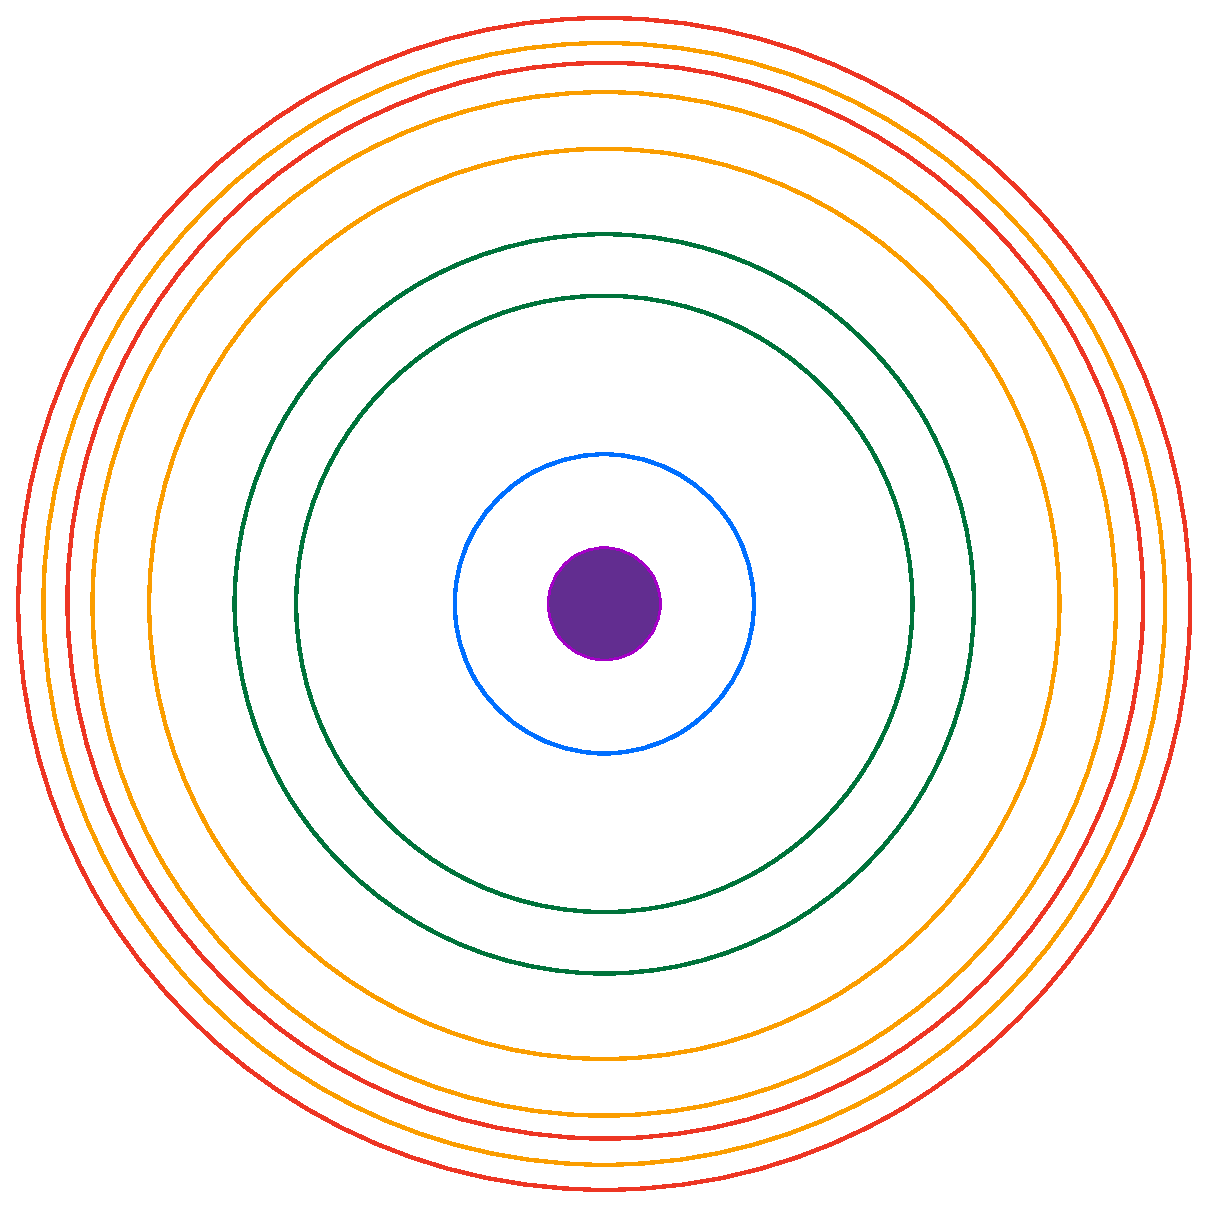
\includegraphics[width=1.0\textwidth]{Figures/orbitals.eps}
\caption{\label{fig:orbitals} Stylistic representation of atomic orbitals, showing levels 1 (blue), 2 (green), 3 (orange) and 4 (red). The difference in energy levels becomes less pronounced further out, to the point where difference in orbitals within these levels becomes greater than those between them by level 4. It is for this reason that the highest energy orbitals of level 3 (3d) are higher in energy than the lowest energy orbitals of level 4 (4s).}
\end{figure}

Atoms which use these d orbitals --- the transition metals --- have unusual properties not encountered in previous atoms as a consequence. And it is precisely these properties that make them so useful to proteins, and why evolution has driven proteins to acquire them.

\subsection{Transition Metals}

Transition metals are often employed as cofactors by proteins, particularly in catalysis. As they occupy a different region of electron configuration space than the organic non-metal atoms that make up the biological amino acids (for reasons just outlined), they can provide functionality that would otherwise be unavailable.

Atom's `prefer' to have full energy levels and sub-energy levels - in the sense that if they are in an environment which draws electrons away from it (an oxidising environment) it will be energetically favourable to lose whatever number of electrons causes it to fall back to the last filled level, emptying the highest energy level. Likewise, if in an electron-rich environment in which electrons are `pushed' to the atom (a reducing environment), they will prefer to take only the precise number of electrons which fills the current energy level.

For elements below scandium, this is straightforward - energy levels are far apart, and there is generally only one clear point to fall back to or advance to. Sodium for example, has a single 3s electron, so when in an oxidising environment it can relinquish this one electron, and become Na+. It has a single oxidation state.

Once d-orbitals start being filled however, this becomes less straightforward. Rather unintuitively, when it comes to \emph{losing} electrons, the 4s electrons are the highest energy, and these will be lost first. Therefore most atoms with unfilled d-orbitals can adopt the 2+ oxidation state. The d-orbitals are rather close in energy level, so if there is further oxidative pressure, these can be lost too. This property of having multiple stable oxidation states is one of the chief characteristics of transition metals. It is partly for this reason that transition metals are so widely employed by evolution as protein cofactors, particularly in proteins which catalyse reactions - enzymes. A common mechanism for catalysing a reaction is to stabilise an otherwise very thermodynamically unfavourable intermediate that might have a strong charge associated - by using a chemical species which can have one oxidation state in its native state but which will happily switch to a more oxidised form, the excess charge from the reaction intermediate can be temporarily `stored' in the cofactor, stabilising the intermediate.

As cations, the transition metals also act as efficient Lewis acids - they can accept lone pairs of electrons. This is also useful in catalysis as it can stabilise intermediate structures by withdrawing excessive negative charge from them. This achieves a similar effect, but do so using a different mechanism. The metal atom is not being oxidised, 

Another curious property of atoms with partially filled d-orbitals is the so-called breaking of degeneracy. In a single, uncharged atom of such elements, the five d-orbitals are said to be degenerate, in the sense of having identical energy levels. This is also true when oxidised, but when these charged ions interact with a solvent molecule or other ligands, some d-orbitals end up closer than others to the orbitals of the incoming ligand, entering a higher energy state than the others. The previously uniform d-orbitals split into two slightly different energy levels, and the previous degeneracy is said to have broken.

This confers some unique properties on these elements - most visibly that of colour. The electrons will prefer to occupy the lower energy d-orbitals, but the energy gap between them is small enough as to be in the visible light range, so light passing through a solution of these ions will absorb some wavelength of them.

It also means that different ligand geometries are associated with different changes in energy, meaning that certain geometries end up being preferred over others. This has implications for proteins, which must fold in such a way that the liganding residues adopt the correct geometry.

Unsurprisingly then, many proteins have evolved to take advantage of these useful properties of transition metals by presenting binding sites on their surface that will acquire one of them. This is generally done by bringing residues with available lone pairs into close proximity to each other, in an arrangement that matches the dimensions and orbital geometry of the desired metal, meaning that the geometric properties of these binding sites tend to match the particular properties of the metal atom they are adapted to. Each metal has its own particular properties arising from its electron configuration, and zinc's are some of the most atypical.

\subsection{Zinc's Unique Properties}

Though a transition metal in the sense that it ten d-electrons but no 4p electrons, it is an unusual one - to the point where it is often not even classified as one \footnote{It is not particularly worthwhile to debate whether zinc is or is not a transition metal objectively --- transition metals are an artificial category invented to serve a particular purpose, and the edges of that category are blurred. By some definitions it is, but other definitions it isn't. What really matters are its objective physical/chemical properties, not the name of the category humans have assigned it to based on those properties.}. Many of the properties of transition metals derive from \emph{partially filled} d-orbitals, which zinc does not have. The five fully filled d-orbitals are relatively stable, meaning it can only really be oxidised to 2+ by losing its 4s electrons, so it has just one oxidation state. Electrons cannot be `promoted' from one d-orbital to another in solution as all spaces in the orbitals are already filled, so it has no colour or spectroscopic activity when in solution. At first glance, zinc would appear to be rather unremarkable metal, unworthy of much consideration by evolution.

However, the data show otherwise. About 10\% of all proteins in the human genome are zinc proteins with a zinc binding site \cite{andreini2006counting} - the second most abundant such metal after iron. It is also the only metal found in all classes of enzyme. Clearly, evolution has found zinc very useful.

In fact it is precisely that unremarkableness that has made zinc so attractive. Having just one oxidation state may mean that it cannot hold onto an electron mid-reaction, but it also means that the ion will retain its electronic properties in a wide range of reducing environments - and its status as a particularly good Lewis acid means it is still very useful in catalysis. 

Its lack of spectroscopic activity may make zinc solutions colourless, but the same arrangement of d-orbitals that causes this also means that there is no energetic penalty for zinc coming out of solution (where it is octahedrally coordinated) and into the binding site because such a transition is accompanies by a rearrangement of the orbitals geometrically. In the case of metals with incomplete d-orbitals forces more of the orbitals into higher energy states. For zinc, there is no energetic penalty in moving from the octahedral geoemtry associated with solvation by water, to the (typically) tetrahedral geometry of protein binding. This equivalence in `Ligand Field Stabilisation Energy' gives zinc an advnatage from the protein's perspective \cite{lachenmann2004zinc}.

As a somewhat unusual metal cofactor, the corresponding zinc binding sites that proteins form around them also have unique properties, distinct from those of other cofactors, and other transition metals.

\section{Properties of Zinc Binding Sites}

What do zinc binding sites `look like' from a structural point of view? What are their properties at the atomic scale?

These questions were addressed by researchers from the very first crystal structures, and continue to be a topic of research today. The properties of zinc binding sites that distinguish them from other spatially proximate clusterings of residues are ultimately what must be used to predict them, so the advances in this field are crucial to any zinc binding prediction model. The history of our understanding of these properties will be reviewed here.

By the middle of the 1980s, a number of structures had been produced and already a few general themes that would recur over and over again were observed. Catalytic sites tended to have three protein ligands and one water ligand, whereas structural sites generally had four protein residues, for example. One of the first reviews in this area to examine the structures obtained so far identified coordination by sulphur and nitrogen, and tetrahedral geometry, as the two defining characteristics of zinc binding sites \cite{williams1987biochemistry}. With the benefit of hindsight we can see that this is a slight simplification, but it shows that a consensus about `typical features' was beginning to form. Another early review would go on to list most of the basic properties of zinc binding sites we now know - their division into structural and catalytic sites, the near ubiquity of water in catalytic sites, the much stronger preference for tetrahedral geometry in structural sites than in catalytic sites, and the preference for histidine, cysteine, aspartate and glutamate residues \cite{vallee1990zinc}. These properties would be repeated and elaborated upon by a number of similar reviews in this period \cite{tainer1991metal,vallee1992functional,coleman1992zinc}.

The more structures that were available, the more detailed the inferences that could be made became. A series of reviews looked at typical atom geometries in cysteine binding \cite{chakrabarti1989geometry} and histidine binding \cite{chakrabarti1990geometry}, and while both papers looked at metal binding generally rather than zinc, in both cases the observations were found to be largely metal-agnostic. It was shown that cysteine generally coordinated the metal such that the Zn---S-C-C torsional angle is either 90$^\circ$ or 180$^\circ$ , and that histidine residues generally coordinate the metal via their NE2 nitrogen atom, with the metal lying in the histidyl plane.

Another structural characteristic of zinc binding sites - and indeed metal binding sites generally - was the `hydrophobic contrast' that seemed to exist around them \cite{yamashita1990metal,gregory1993prediction}. Briefly, this is the observation that metal atoms in a protein tend to be surrounded by a shell of hydrophilic atoms (as might be expected), but that these were in turn surrounded by unusually hydrophobic atoms (measured against the average `background' hydrophobicity of the other residues). This could be implemented as a function of coordinates, which would be at a maximum when centered in such a concentric sphere. It was shown that maxima of this function would cluster around metal binding sites.

Whilst it might be expected that zinc binding sites would have some kinds of structural consensus, it is not immediately obvious that they should have any kind of predictable sequence patterns. However in 1989 it was shown, albeit from a relatively small dataset as existed at that time, that catalytic zinc binding sites seemed to have characteristic ``short and long spacer sequences" \cite{vallee1989short}. That is, the three residues that make up catalytic binding sites seem to be made up of two residues separated by a small stretch of amino acids - around five - and a third residue that is much more distal on the sequence. They proposed that the first two residues were acting as a nucleus, a proto-site that is stabilised by the third residue. This pattern was confirmed by later studies, with the short spacer being found to be generally 2 to 7 residues long \cite{patel2007analysis}.

This was not however the \textit{first} sequence motif associated with zinc binding sites - a few years previously a curious pattern of residues in a transcription factor sequence led to the discovery of a new class of zinc protein, and the creation of a entirely new field of genome engineering.

In 1985 it was observed that a particular transcription factor in the model organism \emph{Xenopus oocytes} was a zinc protein, and moreover that it seemed to be made of globular subunits of rouhgly equal mass, each with a repeating C...C...H...H motif \cite{miller1985repetitive}. They hypothesised that perhaps this particular transcription factor was essentially a string of zinc binding domains --- referred to as `fingers' --- each stabilised by a zinc atom at the base. The very regular repeating pattern of thirty residues, each with these four residues in the the same location, was key in uncovering these `zinc fingers'. While not initially thought to be widespread, in the months and years that followed, more examples of these genome-interacting proteins with similar sequence motifs were identified \cite{payre1988finger}. Finally, in 1989, the structure of the original zinc finger was solved, largely confirming the initial speculations about the structure of this protein, and the role of zinc within it --- the domain was a finger-like projection which could bind DNA bases at the tip, and which was stabilised by a C2H2 zinc binding site at the base.

The field continued to grow - by 1998 there was thought to be at least 500 zinc finger proteins, and possibly as many as 1\% of all mammalian genes \cite{mackay1998zinc}. Much of this field is concerned with the `fingertip' end of zinc fingers, which actually implements the DNA-recognising properties, though for the purposes of this project it is the base that is of more interest. There are a few points to takeaway from this brief digression. The first point, which will be returned to in the section of zinc binding site prediction, is that the zinc fingers were discovered because of a characteristic \textit{sequence} pattern, emphasising that such prediction is both possible and potentially offers many insights. The second is that until this point, much of the interest in zinc binding sites was in catalytic zinc binding sites - there were fewer structural sites available to study, and most reviews from this period addressed them last, if at all. From this point on however, many more became available to study, and it became clear that they were responsible for much of zinc's ubiquity in the proteome.

Most of the early work on characterising the typical properties of zinc binding sites was done by manually surveying the crystal structures available and drawing conclusions from them. But as the 1990s wore on and the number of such structures available reached the hundreds, this became increasingly impractical. Instead, from this point onwards, the sites would have to be collated algorithmically from the Protein Data Bank \cite{berman2000pdb}.

The first such database survey was in 1998 - they found 387 zinc proteins, and after excluding some on quality and experimental technique factors, they were left with 111 \cite{alberts1998analysis}. Some of their findings were in line with what was already known - the three residue/one water combination for catalytic sites, the preference for tetrahedral geometry, histidine's preference for one nitrogen over another (by a ratio of 70:30, they found). They also identified a new almost ubiquitous motif across zinc binding sites which they call the `elec-His-zinc' motif whereby zinc is liganded by a histidine which in turn forms a hydrogen bond with an electron donor of some kind.

This was followed by similar reviews \cite{roe1999zinc,laity2001zinc,grishin2001treble,harding2001geometry,krishna2003structural}, showing similar results - that zinc-ligand distances are similar to those found in small molecules, and further sub-categorising the ever increasing number of zinc finger proteins.

Increasingly, the modes of classification were becoming more sophisticated too. Initially, two kinds of binding site were recognised - catalytic sites, which catalysed some metabolic reaction, and structural sites, which did not and just stabilised structure. Later came the recognition that some sites required the action of multiple metals in a single functional unit - either multiple zinc atoms, or a zinc atom in conjunction with another metal atom. From 2001, a fourth kind was recognised - interface binding sites \cite{auld2001zinc}. It had been known since the early days of insulin research of course that in some cases zinc atoms could stabilise polymeric structures, but by this point there was enough data to classify these as their own category, with their own properties - that cysteine is very underrepresented in them, that stabilisation is often done by beta sheets rather than alpha helices (common in other zinc binding sites), even evidence that these sites could also have catalytic roles in addition to their role in quaternary structure.

A more in-depth look at the differences between catalytic and structural sites even seemed to offer a means of automatically classifying zinc binding sites \cite{lee2008physical}, though generally during this period this was a task done manually. They confirmed that catalytic zinc binding sites tended to have more unusual atom distances and geometries (imposing a `strain' upon them that we will return to in the following section), and looked in detail at catalytic sites' disdain for cysteine residues. They found that a relatively simple method of assuming a site is structural if it is has more than one cysteine residue \textit{and} no water, and assuming it is catalytic otherwise, assigned the correct label in 90\% of cases in their dataset. They also looked at the possibility of using atom distances to classify zinc binding sites, though it must be remembered that when looking at differences in atom distance on the order of single Angstroms, the resolution of the structure you are examining is critical if you are to make sensible inferences.

Atom distances themselves have been a major focus of research. A typical example is a 2007 review \cite{tamames2007analysis} of 994 structures, showing that histidine approaches zinc more closely than cysteine (2.11 \AA \ versus 2.32 \AA \ on average) - with water distances generally somewhere between those two figures. The vast majority of metal liganding atoms are within 3 Angstroms of the metal \cite{dokmanic2008metals}. It has been speculated that some non-zinc metal-ligand distances are longer than might otherwise be expected because of the `Jahn-Teller effect' \cite{doi:10.1002/prot.21601}. This phenonemon, like the Ligand Field Stabilisation Energy that makes zinc so attractive in the first place, results from the different energy levels of the d-orbitals in these metals which distorts them and lengthens the bond. This does not affect zinc binding, but does affect other metals.

The properties of zinc binding sites are not just limited to the metal itself and the residues that coordinate it. It is increasingly recognised that the `secondary shell' around the primary residues are of great importance, by providing a network of stabilising hydrogen bonds around the liganding residues to keep them in their precise orientation \cite{auld2001zinc}. This concept has been extended to the idea of a `Minimal Functional Site' \cite{andreini2011minimal}, proposed as the smallest unit of metal binding that should be used when classifying and studying the phenomenon. The authors in this case used all residues within 5 \AA \ of a liganding residue, but more important is the general idea that the residues around the coordinating residues, which are often part of secondary structure - are crucial to understanding the metal binding itself.

There have also been reviews into the efficacy of these database reviews at all, and the limits of what can be inferred from them. A 2005 review \cite{sommerhalter2005x} suggests that while purely spatial properties, such as the location of the metal ion and its liganding residue identities, can be provided reliably by crystallography, often the precise coordination geometry does not agree with spectroscopic data, and should be treated with caution. They also warn against trying to infer redox state from crystallography, though this does not particularly apply to zinc. A later review \cite{laitaoja2013zinc} pointed out that reported atom distances increase as a function of resolution, and stresses the need to take this into account. They criticise a number of earlier studies for treating unlikely geometries or electronic configuration as `real', or for treating zinc salts and crystallographic artefacts as biologically relevant zinc binding sites.

Finally, it is worth examining the numerous secondary databases that have been created over the past decade and a half relating to zinc binding sites, and which offer a web-accessible means of viewing the properties of zinc (though usually metals generally) binding sites.

\begin{itemize}

\item MESPEUS was one of the first - a general-purpose database of metal binding sites generally, which focused on providing basic geometric information \cite{hsin2008mespeus}, and which allowed basic surveys of atom-length patterns to be carried out.

\item ZifBASE had a more specific focus - this was a database of zinc fingers specifically, and provided much more than structural information from the PDB - sequence information, DNA targets, and physiochemical properties like isoelectric point were also provided \cite{jayakanthan2009zifbase}.

\item Probably the most important resource in this area is MetalPDB \cite{andreini2012metalpdb}, a database of metal binding sites, similar to MESPEUS but with more information and a more sophisticated means of classifying them. They divide their sites among `equistructural sites' - those which have binding sites of similar structure, and within those `equivalent sites' - equistructural sites with the same metal. They place a great focus on the secondary shell, as part of the `Minimal Functional Site' concept they introduced earlier, and have recently updated the resource with a greater focus on apo-structures \cite{putignano2017metalpdb}. They have also provided a number of related resources, such as MetalS3 \cite{valasatava2014metals}, a tool for searching the database via structure pattern rather than keyword, and tools for classifying sites based on similarity \cite{sobolev2013web}. An issue with MetalPDB however is its reliance on asymmetric units in the PDB files they parse - often the raw coordinates of such files represent only the repeating unit of the crystal structure, and the actual `real' biological protein must be assembled from that data using transformation matrices contained with the files. MetalPDB (and most other resources) don't do this, which makes some of their `binding sites' rather unrealistic.

\end{itemize}

Another impression one gets immediately when surveying these resources is that with the exception of MetalPDB, all of these resources have ceased existing - their URLs go nowhere, or their sites are broken beyond reasonable use and obviously not maintained. This is a problem generally with academic software, in which the creation of resources is funded by initial grants However because they do not generate revenue themselves, they need grant funding of some kind in perpetuity if they are to remain online --- which they generally don't have. The solution to this problem is not obvious, and in any case beyond the scope of this PhD.

Other resources are focused more on validating or describing a given metal binding site that it is presented with, such as the coordination geometry classifier FindGeo \cite{andreini2012findgeo}, or the validation tool CheckMyMetal \cite{zheng2017checkmymetal}, which uses known properties of metal binding sites to determine if a proposed binding site is realistic.

\section{How do Zinc Binding Sites Work?}

In parallel with an increasingly clear understanding of the properties of zinc binding sites, theoretical and analytical research was performed on the mechanisms and physics underpinning zinc binding. These two areas of research are complimentary and interconnected, with the properties in large part explained by the physics of the binding sites, and insights into the mechanisms derived from experimental observations.

One of the earliest concepts to be introduced in this area was that of the `entatic state' of metals in biology \cite{vallee1968metalloenzymes}, in the 1960s. Essentially this was the idea that metal atoms in proteins have different geometries and properties than they do in smaller molecules and which they would `prefer' energetically, because the protein backbone is able to impose restraints upon it. It is a kind of `strain' that the protein's overall conformation imposes on the metal and which gives them any unique properties they may posses which are not found outside of biology. For example, it may cause an otherwise unfavourable metal oxidation state to be favoured over another, as can be seen with iron.

This concept was later elaborated upon to show that this strain should be thought of as a two-way process \cite{williams1985symbiosis}. The authors note that ``[They] described the valuable strains induced by the protein in the metal... but they could equally well have pointed to the strain induced in the protein by the metal to it. The overall idea was that of catalytic perfection induced by strain" - a strain which makes the enzyme ``energetically poised for catalysis" \cite{vallee1984metallobiochemistry}.

This is a concept that applies to metalloproteins, but once it started to become apparent just how widely used zinc was in the 1980s, attention began to turn to answering the question of why zinc in particular was of such apparent use to proteins.

One property noted early on \cite{vallee1984metallobiochemistry} was that zinc atoms have a full \textit{d}-shell, making it slightly unusual among transition metals. This means that when ionised, zinc will lose its two 4\textit{s} electrons to become 2+, but there are no other oxidation states that it can realistically adopt - it is `redox inert'. This means that the protein can rely upon the metal retaining its oxidation state regardless of the oxidation environment it finds itself in - a stability whose utility is clear.

Another property of this full d-shell that would be elaborated upon later was the absence of a phenomenon known as `ligand field stabilisation energy' \cite{lachenmann2004zinc,vahrenkamp2007does,maret2009coordination,krkezel2016biological}, as previously outlined. Briefly, this refers to the fact that atoms with incomplete d-shells, like most other transition metals, have preferred coordination geometries and experience energetic penalties if coordination angles deviate from this. If the d-shell is full however, no one geometry is preferred over another, which offers the protein much more flexibility.

Another property of zinc that is revisited time and time again in the literature is zinc's role as a Lewis Acid - it will readily accept electron pairs from electron pair donors \cite{williams1984zinc}. It has been noted that while other metals are superior Lewis acids from a purely chemical standpoint, zinc will more readily form tetrahedral complexes \cite{bertini1985zinc}, making it frequently the Lewis-acid-of-choice.

This effective electron pair accepting that zinc exhibits is important because it is useful wherever zinc is used in catalysis. One of the first zinc enzymes to have its precise mechanism of action investigated was carboxypeptidase A, a digestive enzyme. It was suggested that the water molecule that coordinated zinc as one of its ligands was being `activated' by zinc - its electron pairs were being withdrawn by the metal, making it less able to retain its hydrogens and becoming the more reactive hydroxide. Some structural evidence to support this came from the crystal structure of carboxypeptidase A in complex with a substrate that was known to be hard for the enzyme to digest for reasons at that time unknown. The crystal structure revealed that the substrate was inadvertently looping around and coordinating the zinc atom, blocking the water molecule and accounting for the much slower rate of hydrolysis \cite{christianson1986x}. Another means by which zinc can aid in catalysis is by stabilising any negatively charged intermediate in the reaction by offering a temporary repository for their electrons, as is the case with carbonic anhydrase \cite{christianson1996carbonic}.

Indeed, multiple papers have emphasised this `primed' property of catalytic zinc sites. They have more distorted geometry than the more typically tetrahedral structural sites \cite{roe1999zinc}, the liganding atoms tend to be further from the metal \cite{lee2008physical}, and that they are generally more thermodynamically unfavourable when modelled quantum mechanically \cite{sousa2009zinc}.

The means by which protein residues interact with the metal can also have important consequences. Aspartic acid and glutamic acid are both relatively common zinc binding residues, each doing so via their side chain carboxylate groups. They can either contribute one liganding oxygen atom (`monodentate' binding) or both (bidentate binding) (see
Figure~\ref{fig:dentate}). While early theoretical models suggested that the different modes were determined merely by the other residue identities, with more negative other residues favouring mere monodentate binding \cite{ryde1999carboxylate}, it has more recently been suggesting that a residue may use both. The so-called `carboxylate shift' is theorised to occur when an acidic side chain in a catalytic zinc binding site switches from monodentate binding to bidentate binding so as to keep the number of coordinating atoms around the zinc constant - and thereby reducing the activation energy of substrates entering and leaving the complex \cite{sousa2007carboxylate}.


The reason for the preference for cysteine in structural sites has also received attention. It has been proposed that cysteine residues transfer more charge to the zinc atom, reducing the potency of its 2+ charge and making it less reactive \cite{lee2008physical}. 

Finally, it is worth bearing in mind that zinc does not become `part' of the protein as part of the translation process, but binds to the fully translated apo-protein, in a process whose mechanisms are also crucial to understand. It is possible to compare the apo- and holo-forms of zinc binding proteins using sequence identity - for every zinc binding protein structure you have you search the Protein Data Bank for proteins with a highly similar structure that does not have zinc in the same position. This is precisely what a 2005 review did \cite{babor2005flexibility} in a bid to investigate the mechanisms by which zinc binds proteins in the first place. After looking at 210 apo/holo pairs, they found that often, at least part of the coordination shell is in place before the metal is in place - this is consistent with the `nucleus' theory of the short and long spacer sequences, outlined above. Furthermore, they found that in just 40\% of cases was there any rearrangement of side chains upon metal binding, and in just 14\% of cases did this involve backbone rearrangement. This mode of zinc binding is encouraging of efforts to predict zinc binding from apo-structure, as we will see in the next section.

This zinc binding should not be thought of as permanent either. Metalloproteins are in equilibrium with free metal + apoprotein, and the zinc binding will have an on and off rate like any other complex. While this project is largely focused on proteins where the zinc is essentially a permanent feature of the protein because it is essential for some function, it has been pointed that these are merely proteins where the equilibrium is far to the right, and that all metal proteins lie on a continuum in this regard, with zinc transporters (for example) having an equilibrium further to the left \cite{maret2010metalloproteomics}. This equilibrium constant is determined by the geometry of the binding site, and the secondary shell around the liganding residues seem to play a very large role in fine-tuning this affinity by exercising careful control over the precise positioning of these side chains \cite{kochanczyk2015relationship}.

\section{Conclusion}

Zinc is a crucial metal for a wide variety of functions in biological systems, and across a wide spectrum of organisms. Its chemical properties --- particularly its lack of redox activity which gives it an essentially permanent 2+ charge in physilogical environments regardless of the reducing/oxidising environment it finds itself in --- make it uniquely useful to proteins in carrying out functions that they would be unable to do with either the chemistry of the twenty canonical amino acids (whose atoms are largely electron donors, not acceptors), or other transition metals (whose redox state can alter depending on the environment). Chiefly those functions are the catalysis of reactions as a key component of enzymes, or as a stabiliser of local protein structure --- either a region of a single chain, or at the interface between two chains.

While zinc has other occasional roles, such as as a cellular messenger, these two primary roles require the zinc ion to be tightly and permanently bound to the protein in question. This requires the protein to fold in such a way that it brings together liganding residues for zinc that the metal will have a strong affinity for, due to the geometry and chemical identity of the atoms in question. These zinc binding sites have been examined in every greater detail as the number of zinc protein structures has increased, and certain key properties of the binding sites have been observed repeatedly at both the sequence and structure level.

Some of these characteristic features are the overwhelming use of histidine and cysteine, and to a slightly lesser extent the carboxylate residues aspartate and glutamate (with cysteine being slightly more common in structural sites and the carboxylate residues slightly more common in catalytic sites), the near ubiquity tetrahedral geometry of the liganding atoms, the presence of three liganding residues plus water in catalytic sites and four residues in structural sites, and the typical liganding distances.

Physically, the zinc binding sites seem to rely heavily on a network of stabilising hydrogen bonds holding the primary liganding residues in place, from the secondary residues around them. Binding between the zinc atom and the binding site does not usually rearrange the backbone of the protein much. Zinc largely facilitates catalysis by stabilising the negative charges of any positively charged reaction intermediates, making their existence less thermodynamically unfavourable for the short amount of time that they exist.

The existence of these typical features and well understood mechanisms of action is crucial in trying to predict zinc binding sites from structure or sequence, as it means that there are particular properties to be looked for. The next chapter will examine the methods for making these predictors, and review previous attempts at predicting zinc binding using these techniques.


%\insertfigure[0.5]{name.eps}{short caption}{long caption}{label}
% N.B. do not \end{document} at the end of the chapters

%%%% MACRO DEFINITION %%%%

\providecommand{\pvivax}{P.~vivax}
\providecommand{\pfalciparum}{P.~falciparum}
\providecommand{\cterm}{C-terminus}
\providecommand{\nterm}{N-terminus}

\providecommand{\e}[1]{\ensuremath{\times 10^{#1}}}
\newcolumntype{P}[1]{>{\centering\arraybackslash}p{#1}}
\newcolumntype{M}[1]{>{\centering\arraybackslash}m{#1}}

\providecommand{\refimage}[1]{\figurename~\ref{fig:#1}}

%TC:macro \note [ignore]



%%%%%%%%%%%%%%%%%%%%%%%%%%%%%%%%%%%%%%%%%%%%%%%%%%%%%%%%%%%%%%%%%%%%%%%%%%%%%%%%%%%%%%%%%%%%%%%%%%%%%%%%%%%%%%%%%%%%%
%%%%%%%%%%%%%%%%%%%%%%%%%%%%%%%%%%%%%%%%%%%%%%%%%%%%%%%%%%%%%%%%%%%%%%%%%%%%%%%%%%%%%%%%%%%%%%%%%%%%%%%%%%%%%%%%%%%%%
%													BEGIN
%%%%%%%%%%%%%%%%%%%%%%%%%%%%%%%%%%%%%%%%%%%%%%%%%%%%%%%%%%%%%%%%%%%%%%%%%%%%%%%%%%%%%%%%%%%%%%%%%%%%%%%%%%%%%%%%%%%%%
%%%%%%%%%%%%%%%%%%%%%%%%%%%%%%%%%%%%%%%%%%%%%%%%%%%%%%%%%%%%%%%%%%%%%%%%%%%%%%%%%%%%%%%%%%%%%%%%%%%%%%%%%%%%%%%%%%%%%

\chapter{Computational Techniques} % Write in your own chapter title
\label{Chapter2}
\lhead{Chapter 2. \emph{Computational Techniques}} % Write in your own chapter title to set the page header
In this chapter, the pre-existing algorithms and other computational techniques used to predict Zinc Binding Sites will be outlined.

It will not provide details of specific implementations of them used in this project, or any novel tecnhniques developed - those will be presented in later chapters. It is instead meant to give a general mathematical background to these techniques, and familiarise the reader with the terms that will be used in later chapters.

\section{Machine Learning}

This project aims ultimately to create a predictor - something which can take either a protein structure or a protein sequence, and determine where, if anywhere, are zinc binding regions.

Machine learning is the use of existing data to create predictive models that can take new data and make inferences about it. It `learns' the characteristics of the existing dataset and uses this to predict certain things about the new data. This can be `unsupervised', where the model simply breaks the data into clusters based on its internal structure, or it can be `supervised', where the existing data is labeled with some correct output, and the model learns how to predict the output based on the input characteristics. If the output is a discrete category, this is classification; if it is a continuous value, this is regression.

This project will use supervised learning, because the dataset being used to train the models will already have the locations of zinc binding sites labeled. The inputs and outputs are more open to interpretation however. So far I have framed the problem in terms of entire proteins - the input is an entire protein structure or an entire protein sequence, and the output is the number and location of the zinc binding site(s) that may be present. However this is difficult to translate into machine learning concepts, which is best suited to mapping input objects to either discrete classes or single continuous values. It is not really practical to represent `the number and location of the zinc binding site(s) that may be present' as a category or a number, so instead the problem will be re-framed so that the input is some sub-component of the protein, and the output is a binary class - `yes that component is a zinc binding region` or `no that region is not a zinc binding region'. The problem is therefore a classification problem, with two classes. When a protein is given, it is broken into its various components, each component is run through the model which predicts it as either zinc binding or not zinc binding, and then the net result for the protein as a whole is the list of components that are predicted as zinc binding.

But what should be the components? What inputs will actually be passed to the model? For protein structures, one obvious possibility is simply location in space - every point within the three-dimensional structure is taken (in some specified resolution grid) and passed to the model as an input, which assigns that location a predictive label. This would be comprehensive but time consuming, as there would be many points to check - the number of points could be limited to the protein surface, but there would still be a lot. Another possible means of breaking the structure into components would be to take all the combinations of residues that are known to bind zinc, and treat these as inputs - there could again be very many of these, but fewer than if every point in space were checked. For sequences, there is no equivalent to checking every point in space, as this information is obviously not available and residues nearby in space are not necessarily nearby in sequence. However using the combinations of zinc binding residues is still applicable to sequences.

When the inputs are passed to the model, they are done so as a set of `features'. These are numerical characteristics that the model actually uses to learn what kinds of input belong in which category. These are usually passed to the model as a vector of numbers - classification is just the mapping of vectors to discrete classes. How the inputs are actually represented is determined by feature selection, which must be carried out first. For example, while I referred to using locations in space as inputs in the preceding paragraph, the actual input vector itself wouldn't literally be the three Cartesian coordinates - if that were the case the model would simply try to associate certain distances from the origin of the PDB coordinate system with zinc binding, which would obviously be nonsensical. Instead you pick certain characteristics to measure for a point in space, such as (for example) `number of oxygen atoms within 3 ~{\AA}', and use that number in your input vector. The actual features used in this project will be outlined later.

However, too many features can be a problem. The more dimensions in the vector space the inputs inhabit, the more computationally expensive it can be to process them. Some supervised learning techniques, such as K-Nearest Neighbors, also have poorer performance at higher dimensions because data points are more `spread out' in higher dimensional space. For this reason, dimensionally reduction is often performed, whereby the dataset is transformed into one with fewer dimensions, but retaining the same predictive information. This can be either feature selection, whereby superfluous features which are already highly correlated with other features are removed, or feature extraction, where entirely new features that capture the essence of the original dataset are created.

Once the dataset has been processed, models must be trained. The simplest approach would be to give the model the entire dataset and let it learn from that. However, this can lead to a problem called overfitting, where the model learns details of the training set that are irrelevant - it learns the training set, but is not generalisable to objects not in the training set. To overcome this, the dataset is generally split into a training set and test set, with the latter being held in reserve to assess the model after it has been trained on the training set. If the model is overfit, it will perform much worse on the test set than the training set - if not, the performance on each will be broadly equivalent.

\subsection{Evaluation}

The test set is held in reserve so that the effectiveness of the model can be evaluated, but here `effectiveness' can be defined in a variety of ways. For this purpose, the model can produce one of two outcomes, true or false, so all of the test results fall into one of four categories - true positives (correctly identified as a binding site), false negatives (was a binding site, but not detected), false positives (not actually a binding site, but wrongly identified as one), and true negatives (not a binding site, not identified as one). The first and last categories are the `good' ones, the other two the errors.

The simplest means of grading a model is with accuracy - the total number of correct predictions (true positives and true negatives) as a proportion of all test inputs. This can be a misleading metric however, if the dataset is class-imbalanced - that is, if one class is much more prevalent than the others. This will be the case in this project, as non-zinc binding regions vastly outnumber zinc binding regions. Accuracy is misleading here, because a model which just always predicts the more-prevalent class can get a very high accuracy, despite being completely useless as a predictor of rare states.

Similarly the error rate - the total number of incorrect predictions (false negatives and false positives) as a proportion of all assignments - suffers from the same problem, and should be treated with the same caution in a class-imbalanced problem like this.

Two more meaningful metrics are precision and recall. Precision is the number of true positives, as a proportion of all predicted positives - that is, how many positive predictions were correct? Recall (also referred to as sensitivity) is the inverse, the number of true positives, as a proportion of all actual positives - that is, how many actual positives were identified? A high precision means that false positives are being kept down, with the reported positive cases being mostly correct. A high recall means that false negatives are being kept down, with most of the positive cases being identified.

However these two metrics exist in a balance, with improvements in one causing a decline in the other. The more `eager' the model is to assign a positive prediction to an input, the more of them will be identified and the higher recall will be - but a smaller proportion of the predicted positives will be correct, lowering precision. Likewise, the more resistant the model is to predictive a positive label, the higher precision will be, but the lower recall will be.

Usually it is convenient to have a single value representing the effectiveness of the model, which is done using the F1 Score. This is simply the`harmonic average' of precision and recall - the ratio of their product and sum, multiplied by two.

Another single value measure of model effectiveness is the Matthew's Correlation Coefficient, or MCC. \note{Explain!}

There are metrics which show not how effective the model is in its current state, but how its ability to distinguish one class from another varies over different thresholds. Most classification algorithms can assign a probability of being in one class or the other, and the actual prediction is made by setting some threshold - if the probability is above this threshold, the positive case is predicted. If not, the negative case is predicted. A ROC Curve will show the model's effectiveness changes as this threshold is changed, by plotting false positive rate against true positive rate for every threshold value (to some given resolution). Purely random classifiers will produce a diagonal line - as the threshold is increased, both true positive predictions and false positive predictions will increase by equal amounts because the model can't actually distinguish one class from another at all. The better the model is at making this distinction however, the more this line will curve into the top-left corner, because true positives will increase much faster than false positives in a `good' model.

This graphical ROC curve can be represented in a single metric called the AUC - area under the curve. As the name suggests, this is the area underneath the ROC curve, which will be 0.5 for a purely random model, and 1 for a perfect model. The reason a perfect model has an AUC of 1, is because a perfect model will have some threshold which produces a true positive rate of 1 and a false positive rate of 0, meaning it will touch the top left corner of the plot.

\subsection{Supervised Learning Algorithms}

Supervised learning is the mapping of input vectors to discrete output categories, but there are multiple methods and algorithms for doing this. Each of them is suited for different kinds of problem, and they will be outlined here.

The most basic machine learning algorithm tries to find the parameters to some function of the input values, and then finds a threshold above which the positive class should be predicted. For example, some of the earliest methods to be developed were the Perceptron and Adaptive Linear Unit. These create a linear function, with parameters that are learned during training. In this case `learning' means that the output of this function is evaluated for every input in the training set, the sum of the squared errors is found (which acts as a score of how poorly the model has performed with its current parameters), and the derivative of this squared error function is used to change the values of the parameters using gradient descent. Gradient descent is a common optimisation algorithm that tries to find the minimum of a function - sum of squared errors as a function of input vector, in this case. In practice, a variant of gradient descent called stochastic gradient descent is generally preferred, where a random subset of the training data is used each time. This speeds up the rate of optimisation \note{Why?}.

Linear perceptrons are relatively primitive - they use a linear function and so can only separate data that is linearly separable in the first place, meaning that a line, or plane (etc.) can divide the data in space. However they do illustrate many of the principles that are common to most or all supervised learning algorithms. Many of them have the overall architecture of a function with learned parameters and a threshold, for example. They also illustrate the difference between parameters and `hyperparameters'. A parameter is something the algorithm itself learns, and in this case the parameters are the coefficients of the linear equation, and the threshold value. So for n-dimensional input vectors, there will be n + 1 parameters to learn. A hyperparameter on the other hand is a setting that the user manually sets. For example, the number of passes through the data to make (epochs).

A more sophisticated variant of the perceptron is a supervised learning algorithm called logistic regression. In logistic regression, you still have a linear function whose coefficients the system tries to learn using (usually stochastic) gradient descent. However in this algorithm, before checking the output of the function against a threshold, the value is passed into a second `activation function' which is not linear. In this case the activation function is a sigmoid-like function that maps all inputs to some value between -1 and 1.

Not all classification algorithms take this form of fitting the parameters of a function and then applying a threshold cutoff. Decision trees, for example, divide the input space into regions by a series of branching cutoffs. At the first `node', a dimension and a value which maximally separates the categories is picked, bifurcating into two branches. For each of these two branches, another bifurcation takes place, and so on until the categories are separated. The number of nodes - the depth - is a hyperparameter that is chosen beforehand. This can be a very important consideration - too few nodes, and the algorithm will usually not be able to cleanly separate the data, with low recall and/or precision being achieved. However if there are too many branches, the model will become overfit - it may perfectly separate the training data, but in doing so will learn statistical noise present only in that sample, reducing its ability to generalise.

An extension of the decision tree that can be very effective is the random forest classifier. This algorithm generates multiple decision trees (the precise number being a tunable hyperparameter), each of which is trained on a random subset of the available training data. When a new input is to be classified, each of the trees classifies it according to its own training, and a majority vote is taken to determine the forest's verdict as a whole. This is an example of `bagging', where the noise and errors of individual models are canceled out in an averaging. \note{Is that actually the definition?}

Another supervised learning classification algorithm is K-Nearest Neighbours. This is a slightly unusual algorithm as it has no parameters that are tuned during training. Instead `training' in this case simply means giving it the entire training dataset, which it stores, and this entire dataset is used when classifying new inputs. The k closest vectors in the training set to the input to be classified (the k nearest neighbours) and identified using some distance metric (typically standard Euclidian distance) and a majority vote is taken - the category most represented in the nearest neighbours is the predicted category for the input. The main hyperparameter for this algorithm is the value of k - the number of neighbours to look for. An odd number is usually preferable, so that for binary classification problems there will always be a winner of the majority vote.

K-Nearest Neighbours illustrates a problem that is present in many machine learning algorithms - the so-called `curse of dimensionality'. That is - the more dimensions a dataset has, the harder it is to create effective, predictive models. This is not just because of the extra computational burden. Higher dimensional data is more `sparse' - the distances between objects gets larger. In the case of K-Nearest Neighbours this can be a problem because the nearest neighbours are further away, and the distance of the nearest neighbours approaches the average distance between data points as dimensionality increases, reducing the information content in those neighbours.

There are techniques which can be used to reduce the number of dimensions in a dataset, and they fall into two categories - feature selection and feature extraction.

Feature selection methods identify features in the dataset which can be removed with minimal loss of information. Some features may be very highly correlated with each other for example, meaning that one of them is redundant. Sequential Backward Selection (SBS) is an example of this - you specify the number of dimensions that you want, and remove dimensions one by one until you get to this number. At each iteration, the dimension to remove is determined by some pre-determined criterion, such as which feature has the smallest effect on the model's predictive ability when removed.

\note{Mention Random Forest's ability to do feature selection?}

Feature extraction, by contrast, does not use a subset of the original features, but rather creates an entirely new set of features, transformed from the original ones, that contains the same information in a lower dimensional space. Principal Component Analysis (PCA) is a widely used example, which transforms the original data such that the direction of maximum variance in the original dataset becomes a dimension in the new dataset. This requires the data to be normalised - scaled so that all features are on the same order of magnitude, and with a normal distribution centered at zero. \note{Explain this much better, and the other techniques}

The above supervised learning methods are established algorithms for classifying inputs into categories using single functions. They are widely used, and have been used with considerable success in bioinformatics problems - including the identification of zinc and other metal binding sites (see below). However, there are limits to the discriminatory power of a single function, linear or otherwise, and hence limits to the complexity of the underlying system they can model. Their `capacity' - the space of possible functions they can assume to model reality - is limited.

Rather than utilising a single function, deep learning uses nested functions - each with its own set of parameters - to capture different layers of abstraction in the input data. There is an input layer, which maps the input vector to some intermediate vector which represents some aspect of the input data. One or more hidden layers then acts on these intermediate vectors, eventually passing the data to the output layer which produces a vector representing the model's degree of certainty that the input belongs to each of the possible categories. Each layer acts as a kind of perceptron with a non-linear activation function - if they were all linear then the model as a whole would be linear. This architecture is a neural network, and this is the classical implementation, with every layer fully connected to the layer before it.

Training a neural network requires finding the optimal values for the weights and threshold for each layer. Using the usual technique of defining a cost function and the differentiating this over the various layers would be very computationally difficult to do with the necessary precision. Fortunately a shortcut exists called backpropagation, which allows the neural network to be trained with much fewer computational resources.

There are variants of the artificial neural network (ANN) model outlined above which are better served for different kinds of tasks. Convolutional Neural Networks (CNNs) are a widely used variant that are optimised for processing images and other input spaces that can be thought of as regularly spaced grids in n dimensions. Rather than having every layer fully connected to the layer before it, there are a number of `convolutional' layers in which the perceptrons only connect corresponding localised regions - followed by normal fully connected layers at the end. Rather than standard matrix multiplication, a mathematical operation called convolution is used to determine the forward flow of information through the network.

Another variant is the Recurrent Neural Network (RNN). In standard neural networks, the input data is unordered, and each input is treated in isolation - the network `forgets' what it has just done and treats each input like it was the first. However often datasets have inherent order, and knowledge of what the last input was classified as (or what the last n classifications were) contains important, usable information for classifying the current input. Recurrent neural networks are usually used for sequential data therefore, and are therefore of use in dealing with biological sequences (see below). They operate by adding an extra term relating to previously classified inputs. \note{Explain LSTMs}

Deep Learning is a kind of representational learning - the model itself is learning the features in the input space that are important. This can be seen when processing images - the model's first layer may look for low-level properties of the image, such as regions of high contrast representing borders, the next layer may look at simple combinations of these, and later layers will be sensitive to more high level combinations of visual features. This is inspired by - though does not work in precisely the same way as - the mammalian visual cortex.


\section{Machine Learning to Predict Zinc Binding}

There are still many proteins whose function is unknown. In many cases we only know their sequence, though some of these have had their structure solved experimentally.

One means of determining what function a protein might be intended to perform is to look for certain motifs associated with a given function. If, for example, it can be shown that such a protein had one or more zinc binding sites, that could offer insights into what function the protein performs. Indeed, that is ultimately the goal of this project.

Owing to this clear usefulness, there have been a number of attempts to develop such predictors in the past, dating back to the early 1990s. These methods and techniques form the essential context in which my own project should be understood, and also provide the benchmark of success against which my methods should be judged. Here their progress will be reviewed. They can essentially be divided into two broad categories - prediction from structure and prediction from sequence.

\subsection{Prediction from Structure}

Predicting zinc binding from structure takes the atom coordinates of some protein as its input, and produces as output residues in that structure which are believed to be able to bind zinc if zinc were present - generally along with some estimated probability that this should be the case.

This is perhaps of only limited utility, as very often proteins which can bind zinc tightly will have zinc bound when the structure is solved, and so no prediction is required. Where such methods are of use however is when a protein capable of binding zinc is crystallised without zinc being present - presumably because the researchers didn't know it could bind zinc and so did not provide any in the medium. These apoproteins can be scanned by predictors like this to identify unfilled zinc binding sites. \note{NMR invisibility?}

\note{Other uses?}

The earliest attempt at a general purpose prediction algorithm was the Hydrophobic Contrast Function, developed in 1990 \cite{yamashita1990metal} to detect metal binding sites in general. This began from the observation that metal atoms tended to be surrounded by a shell of hydrophilic atoms, which in turn were surrounded by an outer shell of hydrophobic atoms. They developed a function which took as its input a coordinate in space, and returned a measure of this `hydrophobic contrast' at that location. They showed that by scanning every point in the structure on a grid, evaluating the function at every point, and then ranking the points by their score (the function returned values between -1 for inverted contrast and 1 for desired contrast), the highest scoring points would be clustered at sites of metal binding.

This was the first demonstration that a property of metal binding sites could be used to create a predictive model. However it should be noted that it was only tested on structures with metals already present, not on apoproteins, and the initial observation itself was based on a very small number of metal proteins that were available at that time. It was later expanded upon by combining it with a template-based searching algorithm, whereby the known metal binding sites were represented as stripped-down `templates' of just alpha and beta carbons, and used to search proteins using a simple pattern matching algorithm \cite{gregory1993prediction}. Once a set of three residues matching a known template was found, the hydrophobic contrast function was applied to verify that the binding site was a region of high contrast, which it generally was. This was part of a pipeline for engineering binding sites into proteins, so it didn't require the matching residues to be of any particular type, but the general principle of using known site geometry and hydrophobic contrast properties to look in new structures was still in use.

MetSite was one of the earliest use of machine learning techniques to predict binding sites as we would understand the term today, in 2004 \cite{sodhi2004predicting}. They used artificial neural networks to detect metal binding sites in low-resolution structural models, such as those generated computationally from sequence data. They set themselves a target of having a false positive rate no higher than 5\%, and using this threshold were able to get an 
accuracy of 94.2\% and, more informatively, a recall of 60\% - across all sites. These figures fall to 84\% and 39\% for specific metals, from which they infer that many metals in the structures used are labelled incorrectly. They show that their model can predict metal binding in proteins of unknown function, and in models generated computationally, because the features they use don't use information from the precise positions of liganding atoms, but from outer residues and secondary structure.

Not all attempts at structural prediction have used straightforward supervised learning. The field of molecular dynamics has made important contributions, through the use of empirical force fields which can describe the attraction that a small molecule should experience towards a region of a protein. One such force field, the Fold-X empirical force field, was adapted for use on single atom ligands such as water and metal atoms \note{cite}. Not only were they able to 'decorate' protein surfaces with identified metal binding sites, but the implied affinity of the binding sites reported by the force field correlated closely with experimentally reported affinities where available.

\emph{geometric approaches - graph theory and templates}

\emph{Fold-X}

\emph{Goyal and Mande}

\emph{CHED}

\emph{FEATRUE}

\emph{SitePredict}


One of the more recent algorithms for identifying potential zinc binding sites in protein structures is TEMSP \cite{zhao2011structure}. This is actually reminiscent of some of the earlier work on this problem, in that it uses simple geometric patterns of known zinc binding sites - specifically their alpha and beta carbons - to search target structures without any particular machine learning method employed (though there is a certain amount of parameter training). Here the problem is simplified by creating a library of `residue pairs', where for each zinc binding site obtained from the PDB, they store each pairwise combination of liganding residues (actually just certain properties of them, such as alpha-alpha distance etc.) and then search the target protein for these. Once one is found, other template pairs are superimposed on the structure to find additional liganding residues. They used a stricter definition of `true positive' than previous attempts, and still reported a sensitivity of 86.0\% and a selectivity of 95.9\% in their test dataset - barely lower than the values obtained when testing on the training dataset used to refine their parameters. When applying their tool to a dataset of proteins of unknown function, they found some very promising results - finding 186 probable zinc binding sites. \note{So what?} Unfortunately, the online version of this tool is no longer accessible at time of writing.

\subsection{Prediction from Sequence}

\section{Web Technologies}

A major part of this project's utility to the wider scientific community is the presentation of the data and tools created for it to the world. All of them are available via the web, and various web technologies are used to accomplish this.

\subsection{Django}

Django is an open source Python web framework, used to create database-backed web applications \cite{django}. All database population scripts are written in Python, and use the Django Object-Relational Mapping utilities to populate the database.

\subsection{GraphQL}

GraphQL is an API technology and query language which allows users to construct requests for precisely the data they need - no more, no less \cite{graphql}.

Traditionally, web APIs have used the REST archictecture, whereby every meaningful object is given a URL address. The problem that GraphQL seeks to address with REST is that REST APIs often involve overfetching (you get the full representation of an object whether you want it or not) and underfetching (you have to make multiple requests to get the data you need). With GraphQL APIs, you define your objects using a graph of relationships, and then request exactly the data you need.

GraphQL APIs are used here to provide computational access to both the dataset itself, and to the predictive models.

The Python/django library graphene is used here to implement the GraphQL schemas and API services \cite{graphene}.

\subsection{React}

While the web services provide computational access are useful for programmatic access, for browsing the data initially a website frontend is much more useful. In order to avoid duplication of logic, a JavaScript framework which connects to the existing API is used here - React \cite{react}.

React uses individual components to build up a single page web application, and the React router package is used to create individually addressed pages.

Other JavaScript technologies used on the frontend are the 3D macromolecular visualisation package NGL (used for visualising the zinc binding sites) \cite{rose2015ngl} and the charting library highcharts (used to give an overview of the data) \cite{highcharts}.
%%%% MACRO DEFINITION %%%%

\providecommand{\pvivax}{P.~vivax}
\providecommand{\pfalciparum}{P.~falciparum}
\providecommand{\cterm}{C-terminus}
\providecommand{\nterm}{N-terminus}

\providecommand{\e}[1]{\ensuremath{\times 10^{#1}}}
\newcolumntype{P}[1]{>{\centering\arraybackslash}p{#1}}
\newcolumntype{M}[1]{>{\centering\arraybackslash}m{#1}}

\providecommand{\refimage}[1]{\figurename~\ref{fig:#1}}

%TC:macro \note [ignore]



%%%%%%%%%%%%%%%%%%%%%%%%%%%%%%%%%%%%%%%%%%%%%%%%%%%%%%%%%%%%%%%%%%%%%%%%%%%%%%%%%%%%%%%%%%%%%%%%%%%%%%%%%%%%%%%%%%%%%
%%%%%%%%%%%%%%%%%%%%%%%%%%%%%%%%%%%%%%%%%%%%%%%%%%%%%%%%%%%%%%%%%%%%%%%%%%%%%%%%%%%%%%%%%%%%%%%%%%%%%%%%%%%%%%%%%%%%%
%													BEGIN
%%%%%%%%%%%%%%%%%%%%%%%%%%%%%%%%%%%%%%%%%%%%%%%%%%%%%%%%%%%%%%%%%%%%%%%%%%%%%%%%%%%%%%%%%%%%%%%%%%%%%%%%%%%%%%%%%%%%%
%%%%%%%%%%%%%%%%%%%%%%%%%%%%%%%%%%%%%%%%%%%%%%%%%%%%%%%%%%%%%%%%%%%%%%%%%%%%%%%%%%%%%%%%%%%%%%%%%%%%%%%%%%%%%%%%%%%%%

\chapter{ZincBind - The Database of Zinc Binding Sites} % Write in your own chapter title
\label{Chapter3}
\lhead{Chapter 3. \emph{ZincBind - The Database of Zinc Binding Sites}} % Write in your own chapter title to set the page header

This project is an attempt to develop novel means of predicting Zinc Binding Sites using the known properties of previously identified Zinc Binding Sites. As such, the initial step was to create a dataset of these already known sites.

This is an undertaking that has been performed previously - several times (see Chapter 1). One of the primary reasons that the effort has been duplicated so many times is because in none of the previous dataset generations did the authors make their data publicly available in an easy-to-use resource. Therefore from the very beginning of this project, the intention was always to not \emph{just} create this dataset of Zinc Binding Sites, but to make this database publicly available via a web resource, that would be continually updated with new sites as they become available.

This chapter will describe the creation of that dataset, and the web application that offers users access to the data - ZincBind.

\section{Data Generation}

ZincBind uses as its primary data source the Protein Databank \cite{berman2000pdb}. This contains hundreds of thousands of protein structures, a subset of which contain zinc atoms and which can be inspected to see if a zinc binding site can be identified.

The RCSB web services \cite{burley2020pdb} allow a user to query the entire databank by, among other things, the chemical formulae of its small molecules. The PDB IDs of all zinc atom containing structures can therefore be obtained by issuing a request to these web services for a \verb|ChemCompFormulaQuery| with the formula \verb|Zn|.

If the dataset is being created from scratch, each of these PDB IDs is iterated through in turn to look for zinc binding sites. If the dataset is merely being updated with new structures, only those IDs that don't already exist in the database are used.

\subsection{Structure Inspection}

The algorithm iterates through each PDB code and for each attempts to determine what zinc binding sites are present, if any, and saves the relevant objects to the database once its analysis is complete.

Each PDB ID is analysed within a single database transaction, meaning that the SQL statements are built up by Django throughout the analysis and then executed all at once at the end of each PDB ID analysis. This has two benefits. Firstly, it makes the whole process much faster - there are database records for each atom in the binding site, so opening up database connections, creating a record, and closing the connection multiple times per structure is much more time consuming than just doing that once at the end. Secondly, and more importantly, if the program is interrupted in the middle of building a database, it will essentially rollback to the last fully processed PDB, rather than saving records for half-processed PDBs which could cause errors when the program is restarted.

The structures are requested from the RCSB web servers in the mmCIF file format. This, and all subsequent structure parsing and analysis, are abstracted into the atomium Python library (see Appendix A).

The first processing step with the obtained and parsed structure, is to generate a biological assembly. The raw coordinates of the PDB structure contain the `asymmetric unit', which is often not the way the chains are arranged outside of the crystallisation experiment. Each PDB structure contains a list of possible biological assemblies that can be created from the chains in the asymmetric unit to make a more biologically realistic structure, and each is associated with a list of transformation matrices and calculated metrics. The delta free energy of the assemblies are used to rank them, and the lowest delta free energy assembly that still contains zinc is selected as the `real' biological assembly.

This step is critical. While asymmetric units are perfectly suitable if you are merely concerned with intra-chain features, they are often unsuitable for examining the interfaces between chains. Since many zinc binding sites are between chains, relying on asymmetric units would produce data that is not particularly meaningful.

However it is important to keep in mind that, necessary though biological assembly generation is, it does introduce some problems. Many assembly instructions are simply to get a subset of the chains in the asymmetric unit, which is fine, but some require copies of chains to be created. For example, a structure that starts out with an A chain and a B chain may in its biological assembly have two A chains and two B chains. As there is no established protocol for generating new IDs for these chains (and since creating one would create inconsistencies with other software that uses the data in the ZincBind database, such as the NGL protein viewer), the solution used here is simply to have multiple chains with the same ID. This can cause a number of problems which will be outlined, along with their solution, as they arise in this section.

Once the correct assembly has been generated, the algorithm then checks that the resultant structure is usable, and is not just alpha carbons as some older structures are. If it is such a `skeleton structure', the zinc atom(s) in that structure are saved to the database with an annotation explaining that they don't have a binding site because the PDB was unusable. Note that this is the case whenever a zinc atom is rejected - it is still saved to the database with an explanatory annotation, because by doing this \emph{every} zinc atom in the Protein Data Bank can be accounted for in ZincBind. If this were not done, and a user tried to find a particular zinc atom from the data bank in ZincBind which had not been assigned a binding site, that user would have no way of knowing if the zinc atom was absent because ZincBind had not examined that PDB, or if it was absent because a binding site could not be assigned to it.

Any zinc atoms that are in the asymmetric unit but not the biological assembly (common in cases where the asymmetric unit is just the biological assembly repeated multiple times) are also saved to the database without a binding site, with an explanatory explanation as to why it has none, for the same reason.

The next step is to actually identify all of the binding sites. This is done as follows:

\begin{enumerate}
   \item Identify all metals in the structure. This is done using element names in atomium, but it is here that the first biological assembly related awkwardness must be dealt with. When these assemblies are being generated, sometimes atoms end up superimposed on top of each other - so called `special position' atoms. The correct interpretation of this is that there is just one atom here, not multiple occupying the same position in space, so duplicates have to be removed. This is done by taking all atoms of a given element, comparing it with every other atom of that element, and if the distance between is less than 1~{\AA}, one is removed.
   \item Determine the atoms which ligand each metal in the structure. All atoms within 3~{\AA} of the metal which aren't carbon or hydrogen are determined, and again duplicated atoms must be removed from these using the same algorithm as above (insulin structures for example, often have a chloride ligand which would appear multiple times in the same location otherwise). Once this `cloud' of suitable liganding atoms is obtained, they are ordered by distance to the metal, and for each one a check is made that the angle formed between it, the metal, and any closer atom is not less than 45$^\circ$. If it is, the atom is removed from the set of liganding atoms as it is assumed a coordinate bond would be infeasible if there is another coordinate bond so close.
   \item Remove metals that probably aren't physiologically relevant. Sometimes a metal atom in a model is just there as a consequence of the crystallisation environment, and while it may interact with one or two residues, those residues might not be a `real' zinc binding site in the sense of being an evolutionarily selected combination of residues there specifically to bind zinc. There is no way to identify with certainty which category a given zinc atom falls into from atom coordinates alone, but ZincBind implements a filter whereby if a metal atom has fewer than three main chain liganding atoms, it is discarded as probably irrelevant. Again, those atoms which are excluded at this stage are given an annotation explaining the reason, if they are zinc atoms.
   \item Merge the metals into single binding sites where necessary. So far, all metals have been considered in isolation, though in reality some of them may form co-functional units with each other. To determine if this is the case, the residues/ligands that the liganding atoms are part of are examined and, if two metals share a residue/ligand, they are assigned to the same `cluster'.
   \item Remove non-zinc binding sites. ZincBind is a database of \emph{zinc} binding sites. So far all metals have been considered because some non-zinc atoms may be part of a multi-metal site that contains zinc, so had to be included at every step. However now that the fully processed sites have been generated, those that don't contain zinc can be removed.
   \item Identify the secondary residues of each of the binding sites. This is the set of all residues which are within 3~{\AA} of a primary liganding residue. These residues are saved, along with the details of which atoms mediate these connections. The importance of second shell residues in stabilising the primary liganding shell has been well documented, so identifying how many of these stabilising contacts exist is important information.
\end{enumerate}

Now that the zinc binding sites have been identified, they can be saved to the database. Before this is done however, the chain objects are saved to the database, as these records will be needed when the sites are saved. Any chain in the structure with a residue that is part of a binding site is saved. The sequence used is the full canonical sequence listed in the header of the structure file, not the actual sequence of residues in the model, which may contain missing residues (particularly at the ends of the sequence). These two sequences are aligned using the Smith-Waterman global alignment algorithm \cite{smith1981alignment} so that the liganding residues in the model can be identified in the full sequence, and capitalised.

\emph{Then} the sites themselves are saved to the database, along with records for any metals, residues, and residue atoms. So-called `Chain-Site Interactions' are also saved, which are essentially chains from the point of view of a particular site. While the plain chain objects saved above have residues involved in any binding site highlighted, here only the residues involved in that particular site are. This is important as chains may be involved in multiple sites, but predictive models need to know which residues contribute to \emph{single} sites.

\subsection{Equivalent Sites and Families}

The database as it stands at this point in the algorithm will be a list of zinc binding sites, where each site is considered distinct and separate from all others. This is somewhat misleading, as many proteins appear in the Protein Data Bank several times, and so the binding site(s) in those structures will appear in ZincBind several times. The binding site in (for example) Carbonic Anhydrase will appear in ZincBind many hundreds of times, yet each of these records refer to the same biological unit.

To account for this, ZincBind clusters binding sites into equivalent sites called `groups'. The first step is to cluster the zinc binding chains that were saved as part of the earlier generation process into clusters on 90\% sequence identity, using the program CD-HIT \cite{li2006cdhit}. It is assumed that chains in a chain cluster are functionally equivalent.

The binding sites themselves are then clustered using these chain clusters. Two zinc binding sites are assigned to the same cluster if (1) they are associated with the same chain cluster(s), (2) they have the same residue names in the same order, and (3) their surrounding residue names are the same. These latter two steps are important to ensure that chains with two or more zinc binding sites along them don't have those binding sites incorrectly assigned to the same cluster.

A group object is stored in the database for each of these clusters, and the corresponding zinc binding sites are linked with them. Thus ZincBind stores individual zinc binding sites as they occur in the Protein Data Bank, and unique zinc binding sites in the form of groups.

Binding sites and groups form two components of the three-part hierarchy of data in ZincBind, the third being the family. Each binding site is given an alphanumerical code based on its residue content and count --- so, for example, binding sites with three histidine residues are `H3', those with two histidines and two cysteine residues are C2H2, and so on. These make up the `family' that the binding site. Binding sites are clustered into groups, which are in turn clustered into families based on residue content.

\section{The ZincBind Web Resource}

As already noted, the creation of this dataset was intended to serve both as the primary dataset of this project, and as a publicly available resource. This resource is called ZincBind, and is publicly available.

The database is accessible via a GraphQL API, which allows any specific object, or set of related objects, to be requested in a single HTTP request (see Figure ~\ref{fig:zincbind-api-example}). This is available at \url{api.zincbind.net} and is the primary means of obtaining data from ZincBind in an automated fashion. As outlined in chapter 2, this is created using the Python web framework Django (particularly its Object Relational Management system) and the GraphQL library graphene.

\begin{figure}
\centering
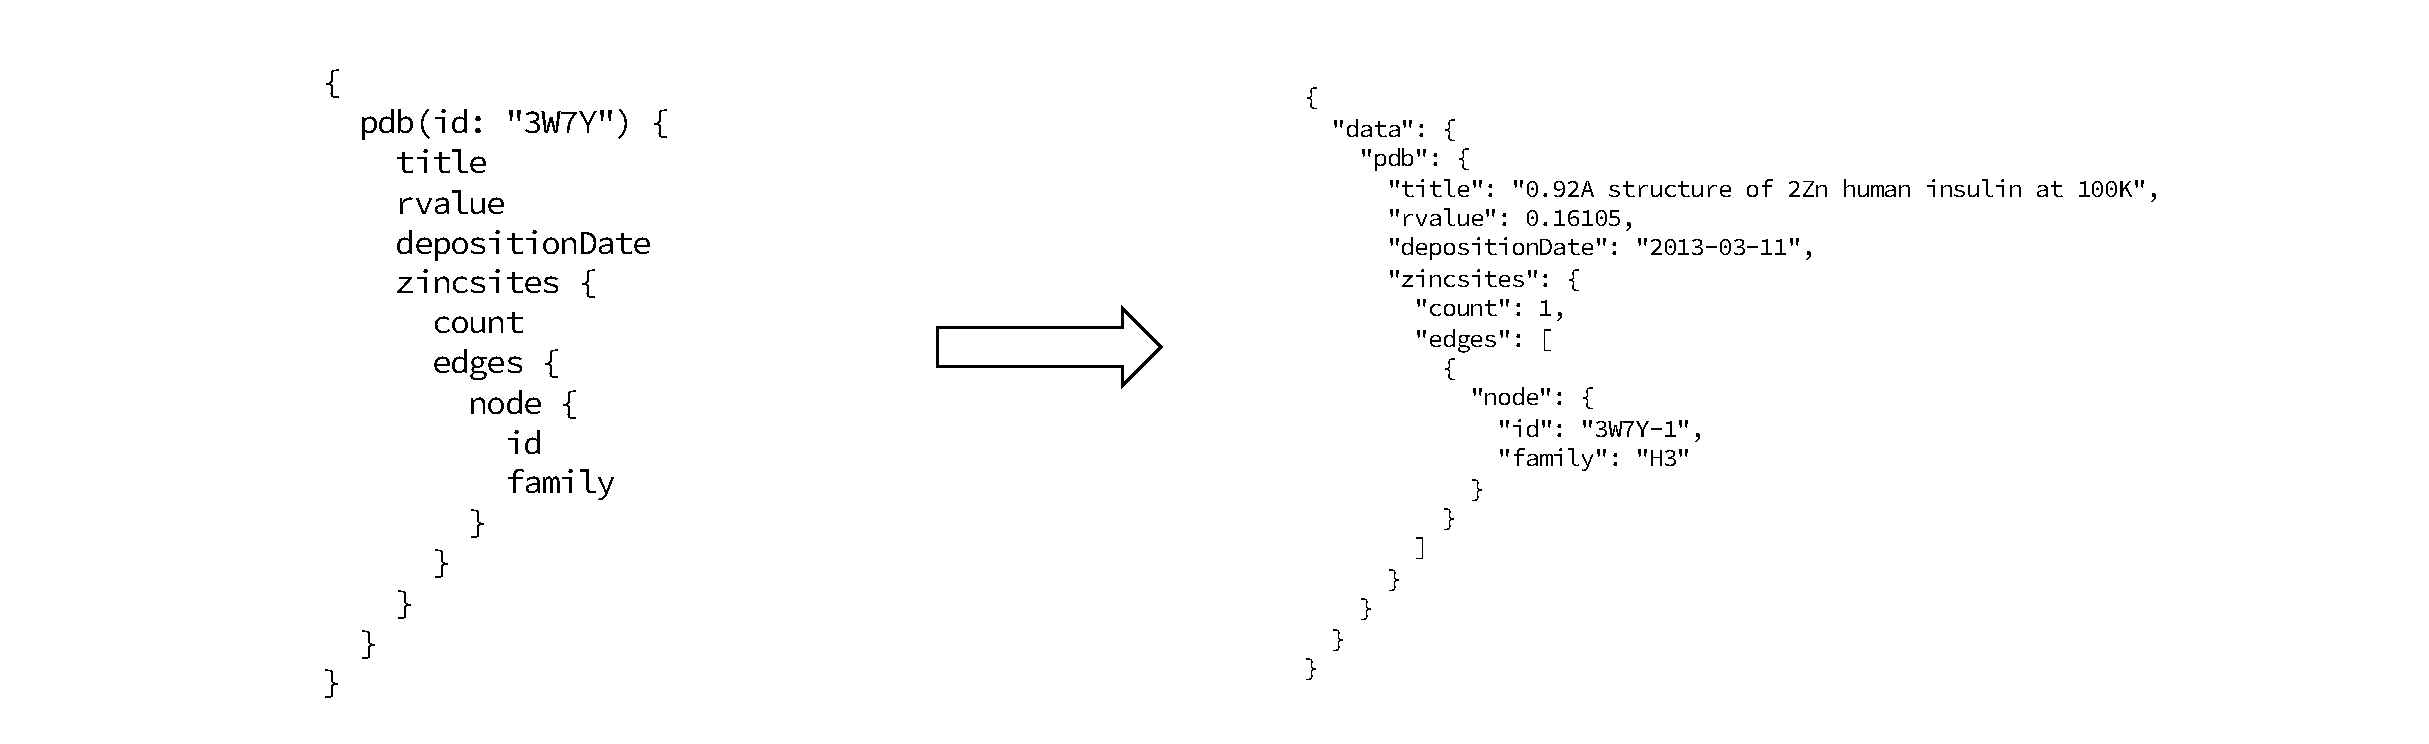
\includegraphics[width=1.0\textwidth]{Figures/zincbind-api-example.eps}
\caption{\label{fig:zincbind-api-example} An example of a ZincBind GraphQL API query
--- in this case for a \texttt{PDB} object,
here requesting all the zinc binding sites within that \texttt{PDB} --- there is
one in this case. In this case the fields \texttt{id} and \texttt{family} are
requested for each, though they also have other fields.}
\end{figure}

More accessibly for casual browsing, there is also a website available at \url{zincbind.net}. This is a lightweight web frontend that interacts with the database via the GraphQL API and presents it to the user graphically. It is a responsive, mobile-first layout created with the front-end framework reach, that adapts to different screen sizes.

The home page (see Figure ~\ref{fig:zincbind-homepage}) contains a short, clear statement of what ZincBind is (a ``database of zinc binding sites, automatically generated from the Protein Data Bank") as well as a brief overview of its key metrics - number of unique binding sites, total number of binding sites, and the number of PDB files the sites are derived from.

\begin{figure}
\centering
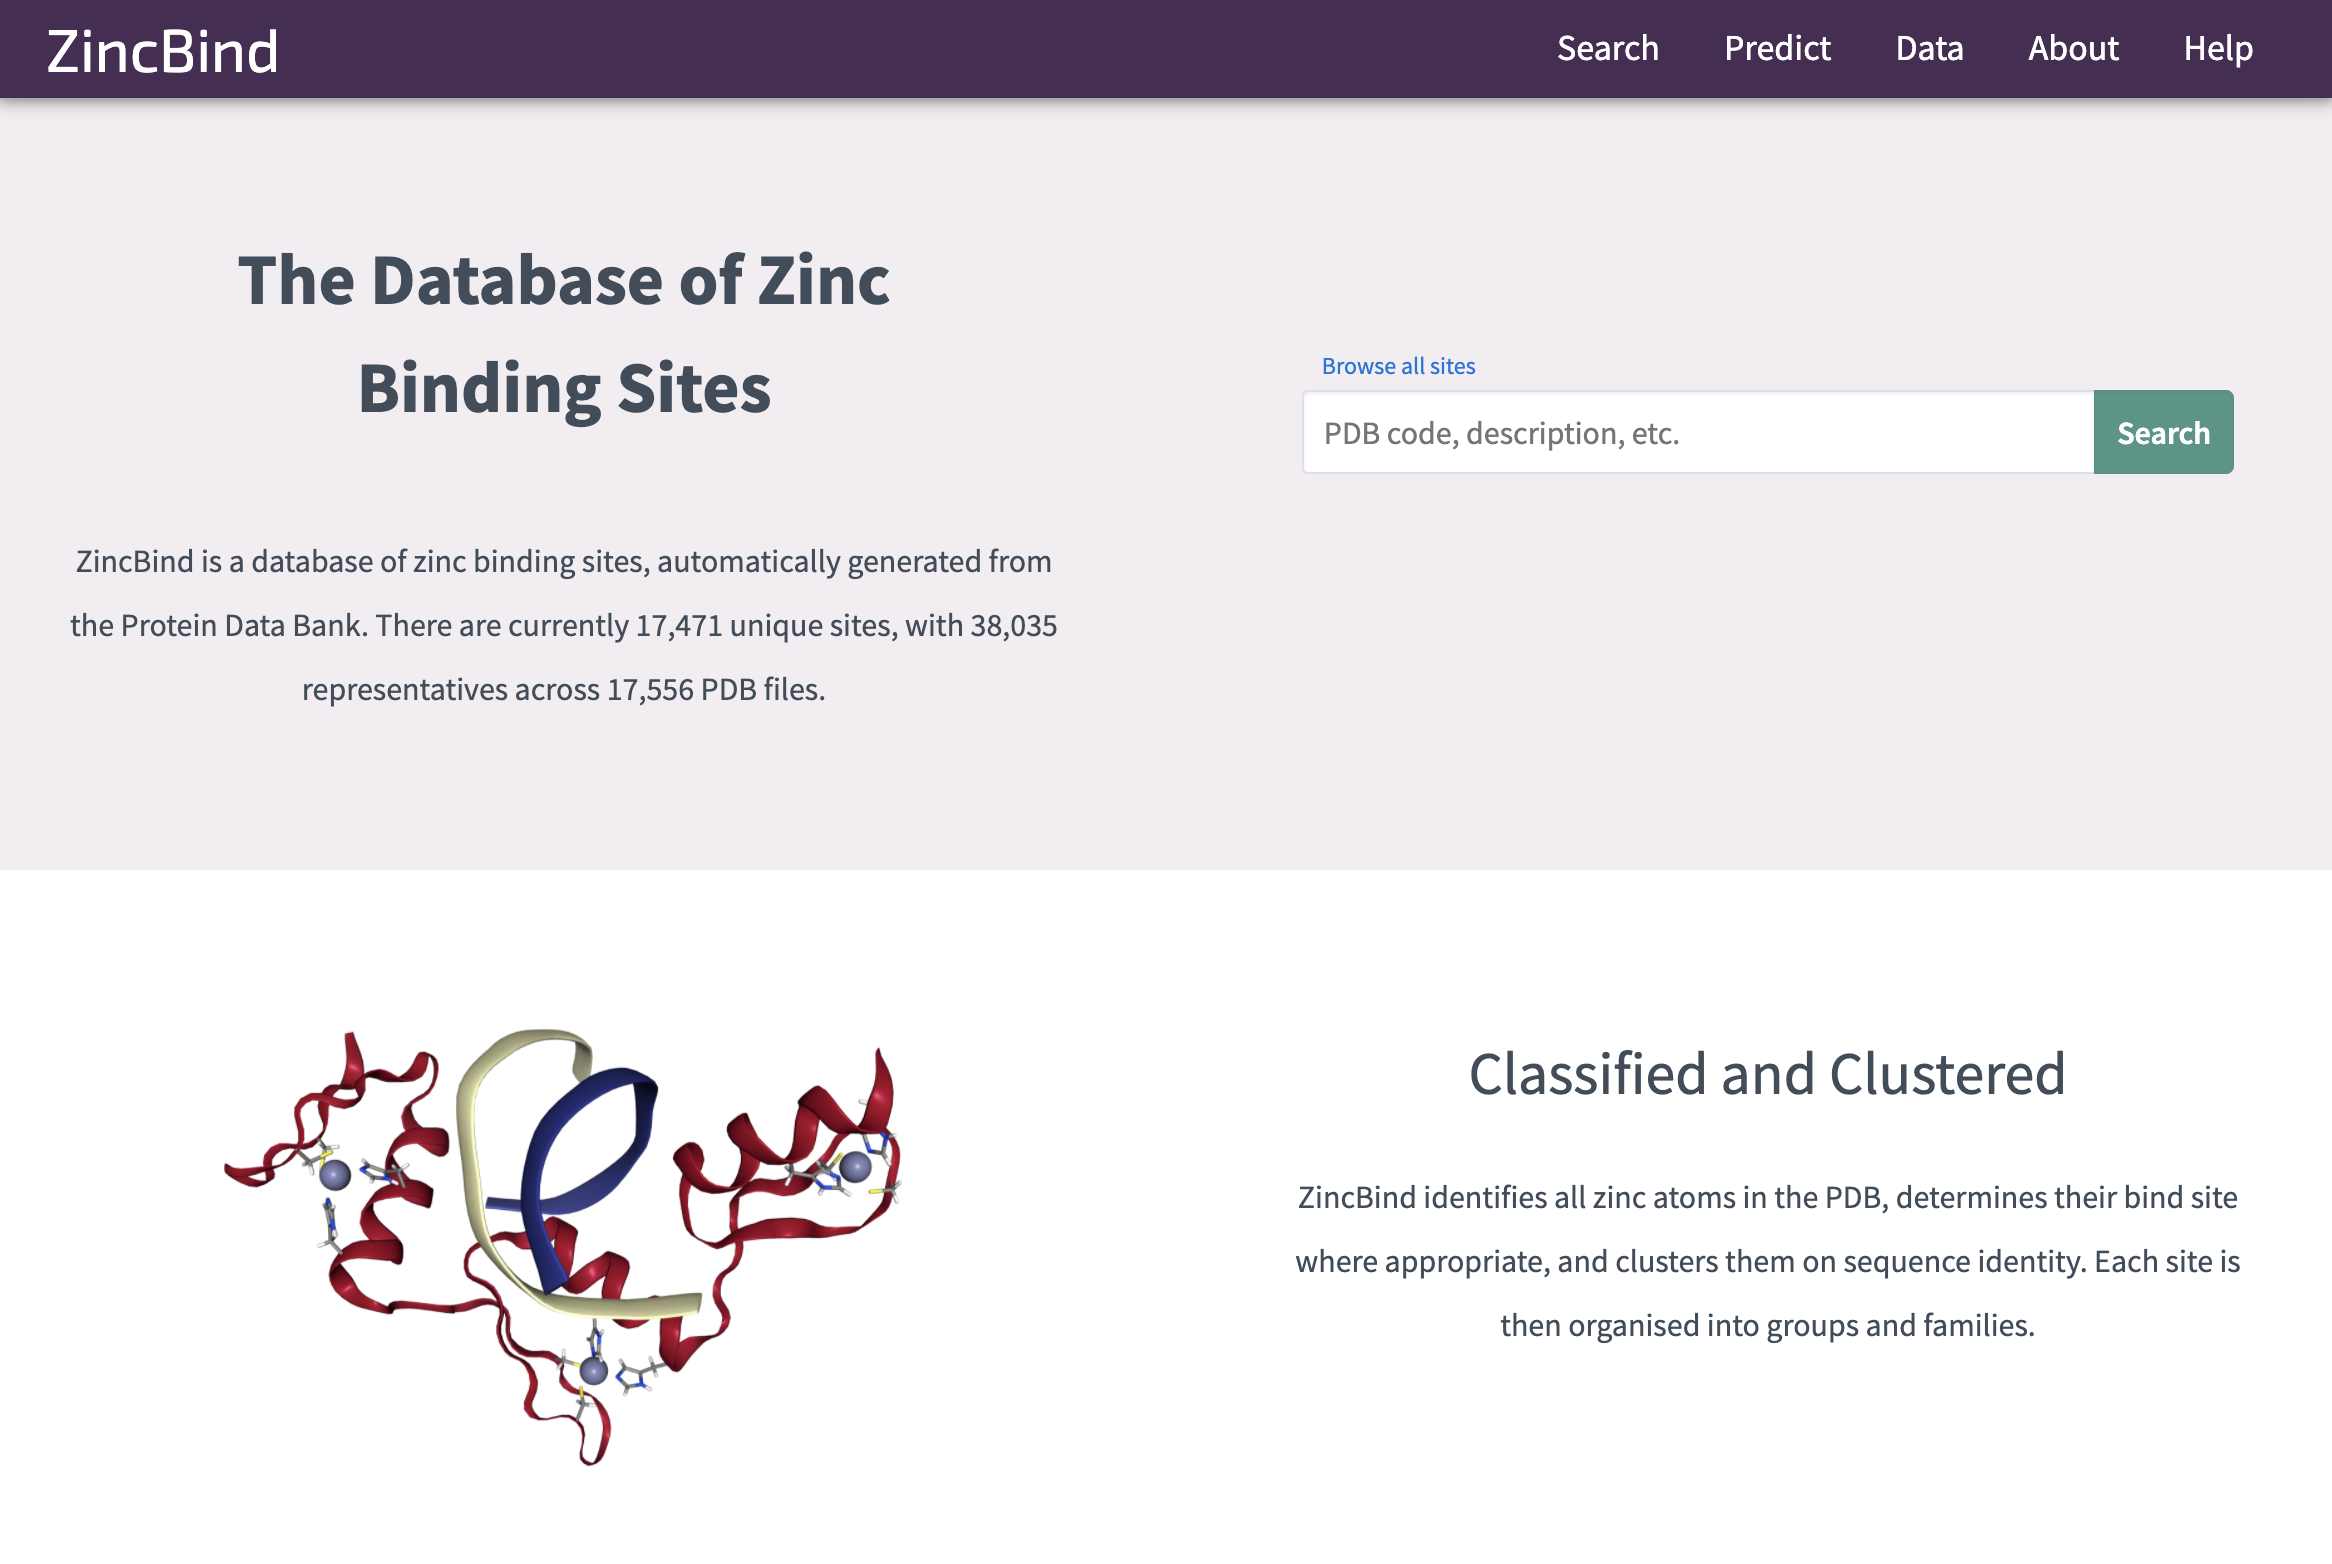
\includegraphics[width=1.0\textwidth]{Figures/zincbind-homepage.eps}
\caption{\label{fig:zincbind-homepage} The home page of ZincBind, showing the
overview statistics in the top-left, and the quick search text box in the top right.
The menu bar at the top collapses on small screen widths, making them accessible via a
drop-down menu on mobile.}
\end{figure}

Searching of the database can be done in one of four ways. Firstly, from the home page, the user can enter a search term that will be used to search multiple PDB fields at once - title, PDB code, classification etc. This is for users who just want to find entries that have any relation to a given term at all, and provides an easy, low-friction way for a user to submit a search immediately.

Secondly, the user can navigate to the Advanced Search page (see Figure ~\ref{fig:zincbind-search}), where they can specify a more precise search by one or more PDB fields. This also allows searching by numeric cutoffs, such as for PDBs below a certain resolution or deposited after a certain date --- essentially any of the PDB metrics that are stored in the database.

Thirdly, via this same page they can search for specific binding sites rather than for containing PDBs. The user can pick the same metrics as for PDBs (sites in PDBs below a certain resolution, with a certain classification etc.) as well as site-specific metrics, such as sites of a particular family, or containing particular residues.

\begin{figure}
\centering
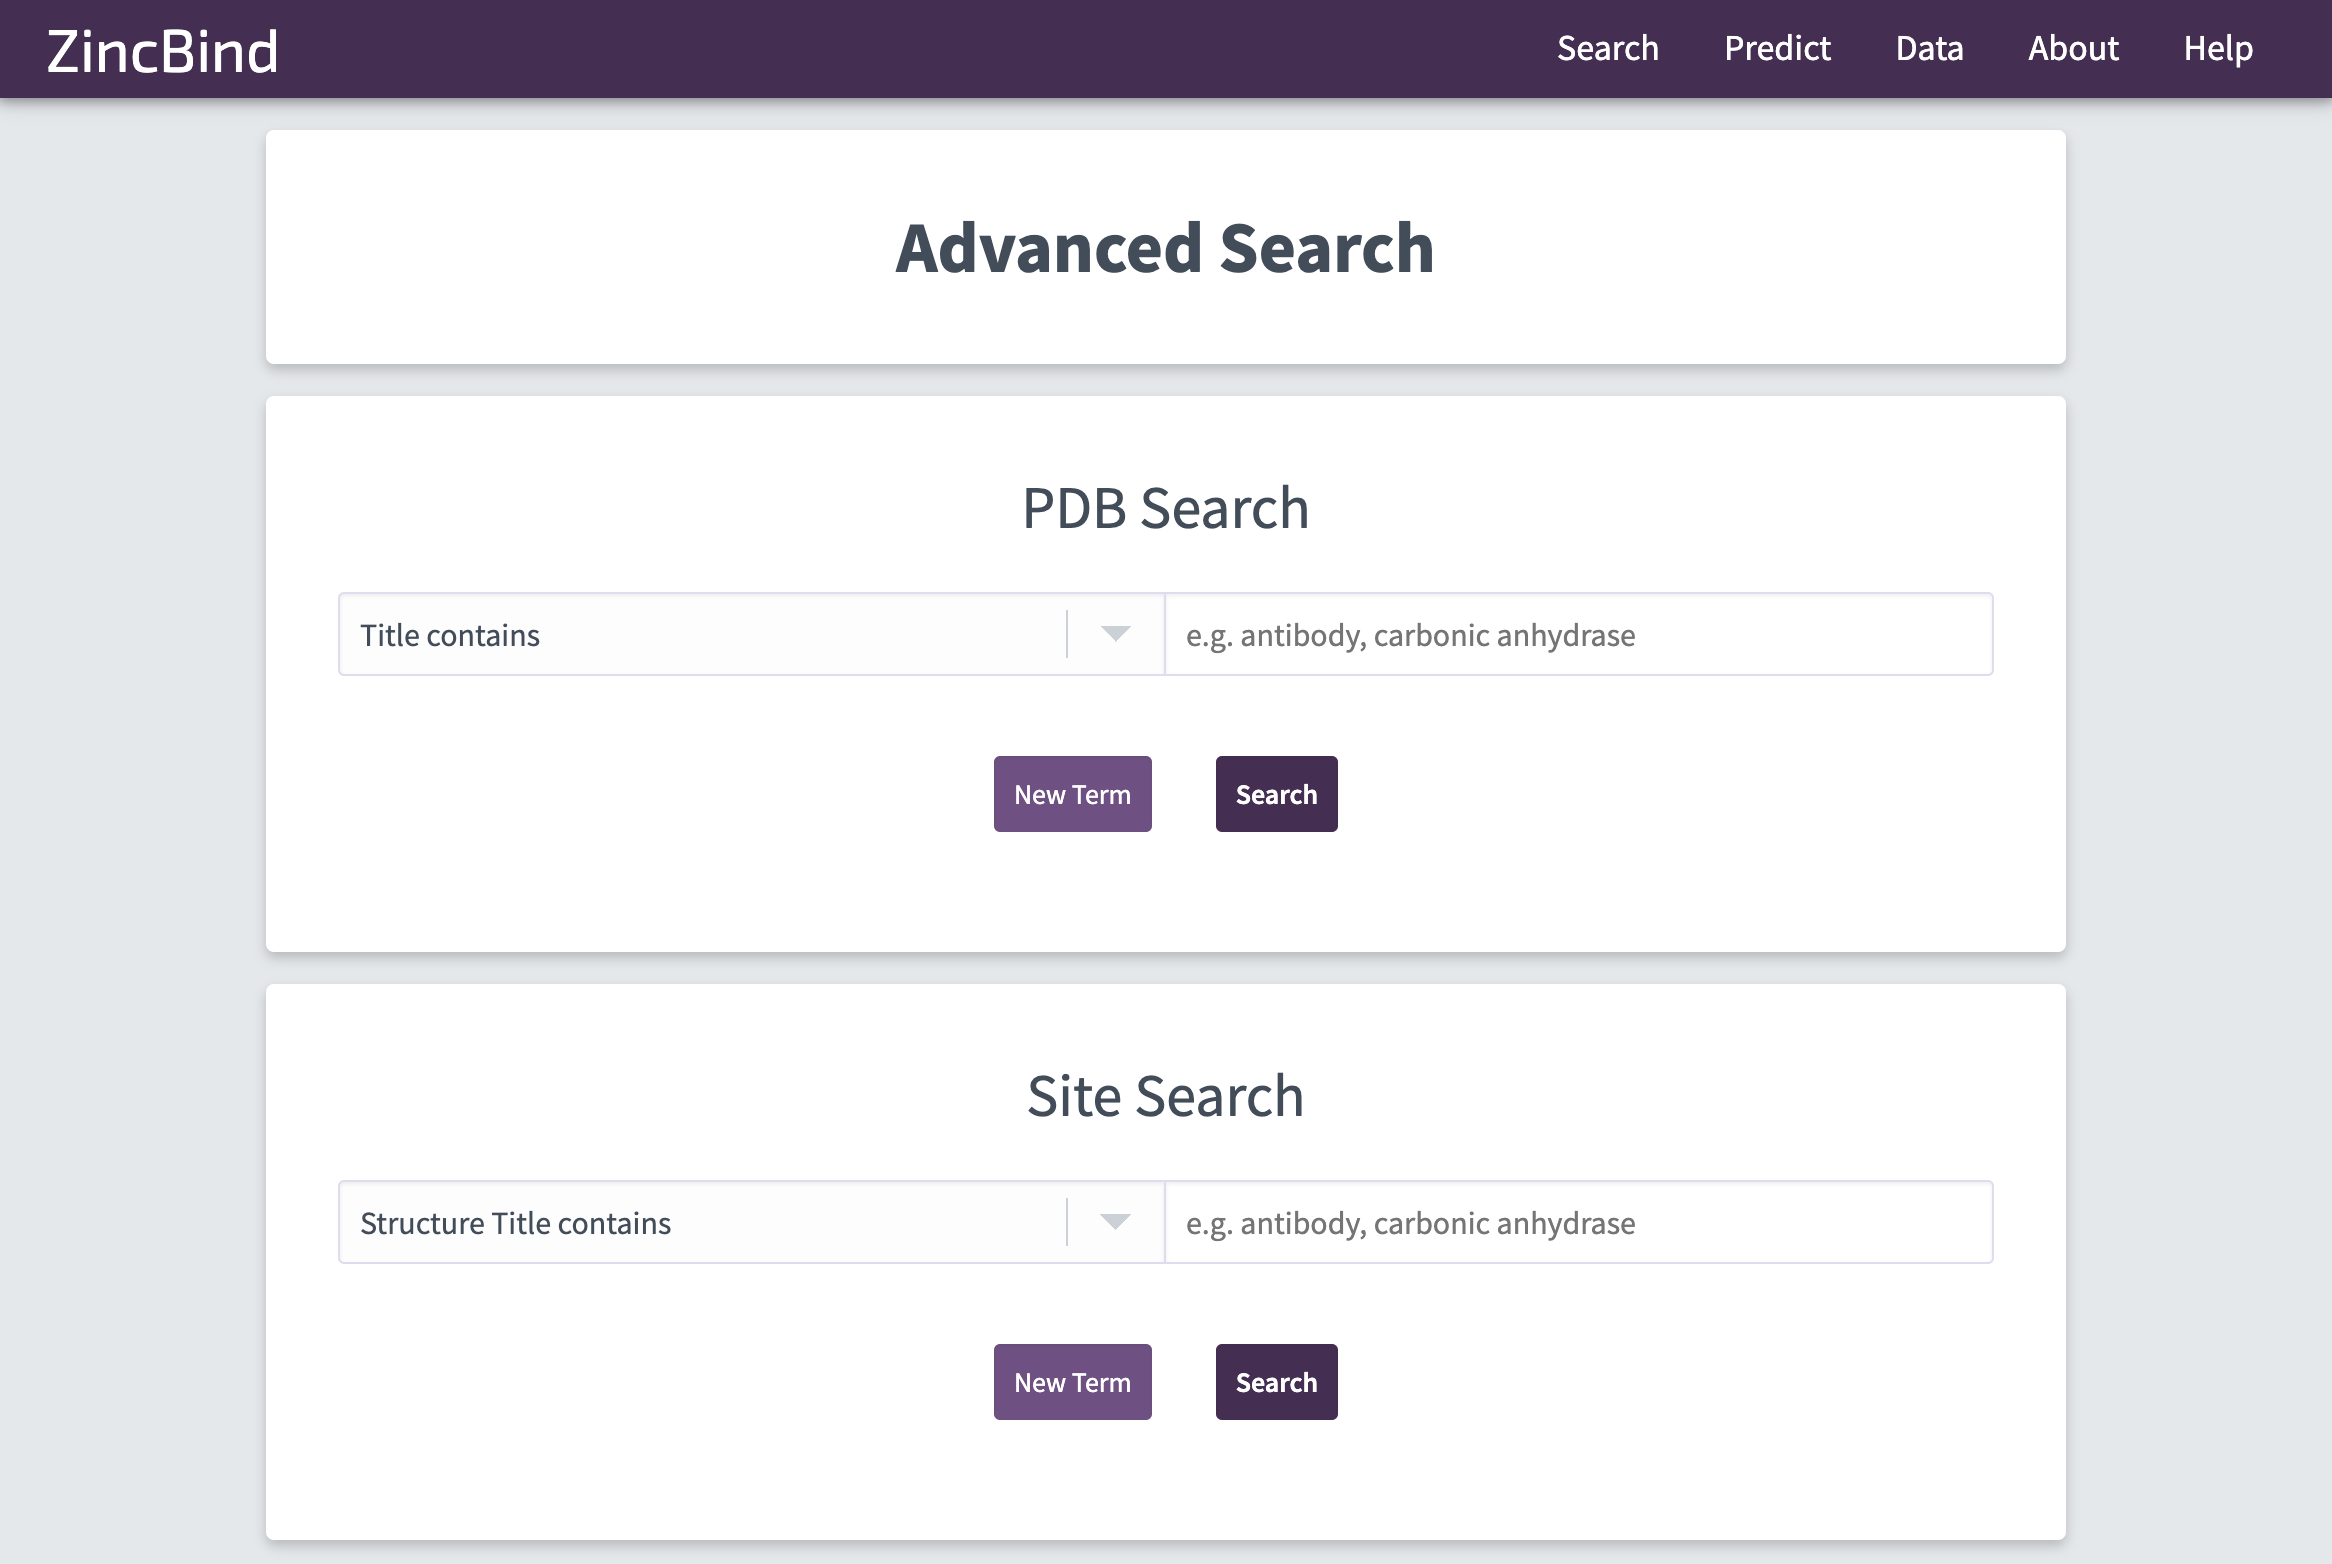
\includegraphics[width=1.0\textwidth]{Figures/zincbind-search.eps}
\caption{\label{fig:zincbind-search} The advanced search interface, allowing searching of
PDB files, or individual zinc binding sites.}
\end{figure}

Finally, the user can provide a sequence and BLAST search the database (see Figure ~\ref{fig:zincbind-blast}). This uses the NCBI \texttt{blastp} binary on the backend, whose JSON output is processed by python functions and exposed via the GraphQL API. This produces chain sequence results (see Figure ~\ref{fig:zincbind-blast-results}), rather than PDB/sites as the other methods do.

\begin{figure}
\centering
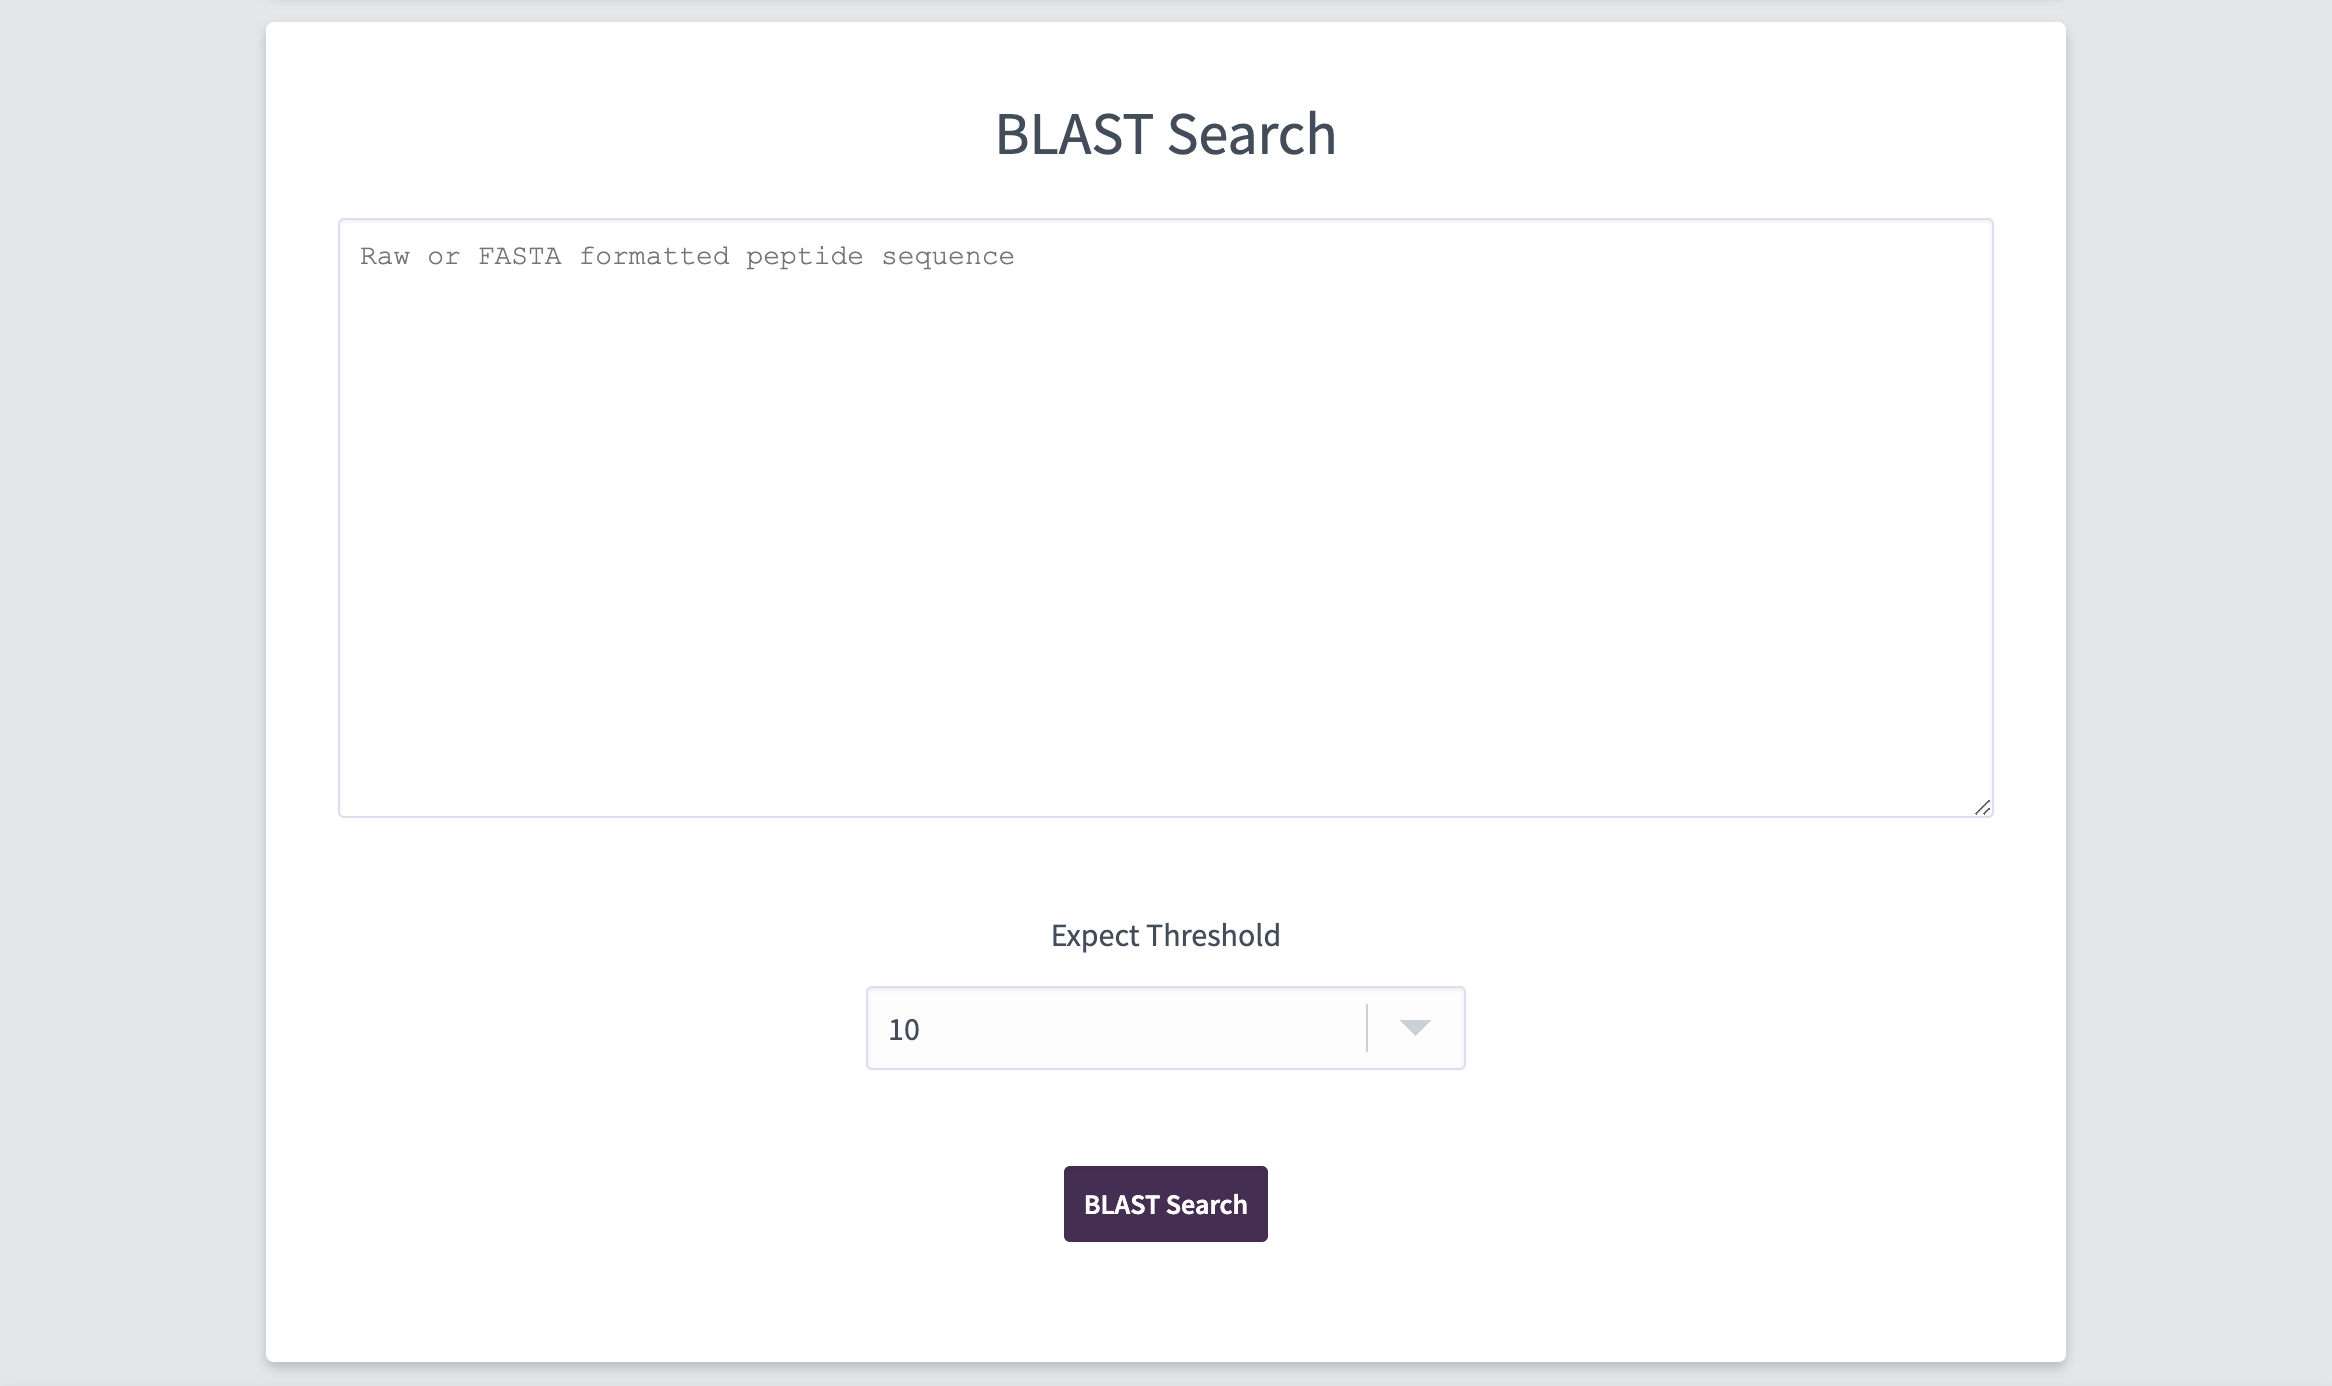
\includegraphics[width=1.0\textwidth]{Figures/zincbind-blast.eps}
\caption{\label{fig:zincbind-blast} The BLAST search interface.}
\end{figure}

The search results for the first two modes of searching are returned as a list of matching PDBs, with binding sites nested within them. Both the PDB and the sites themselves are clickable and will take the user to the page for that entity. Search results can be sorted by a variety of metrics, and are paginated to 25 results per page (see Figure ~\ref{fig:zincbind-results}).

\begin{figure}
\centering
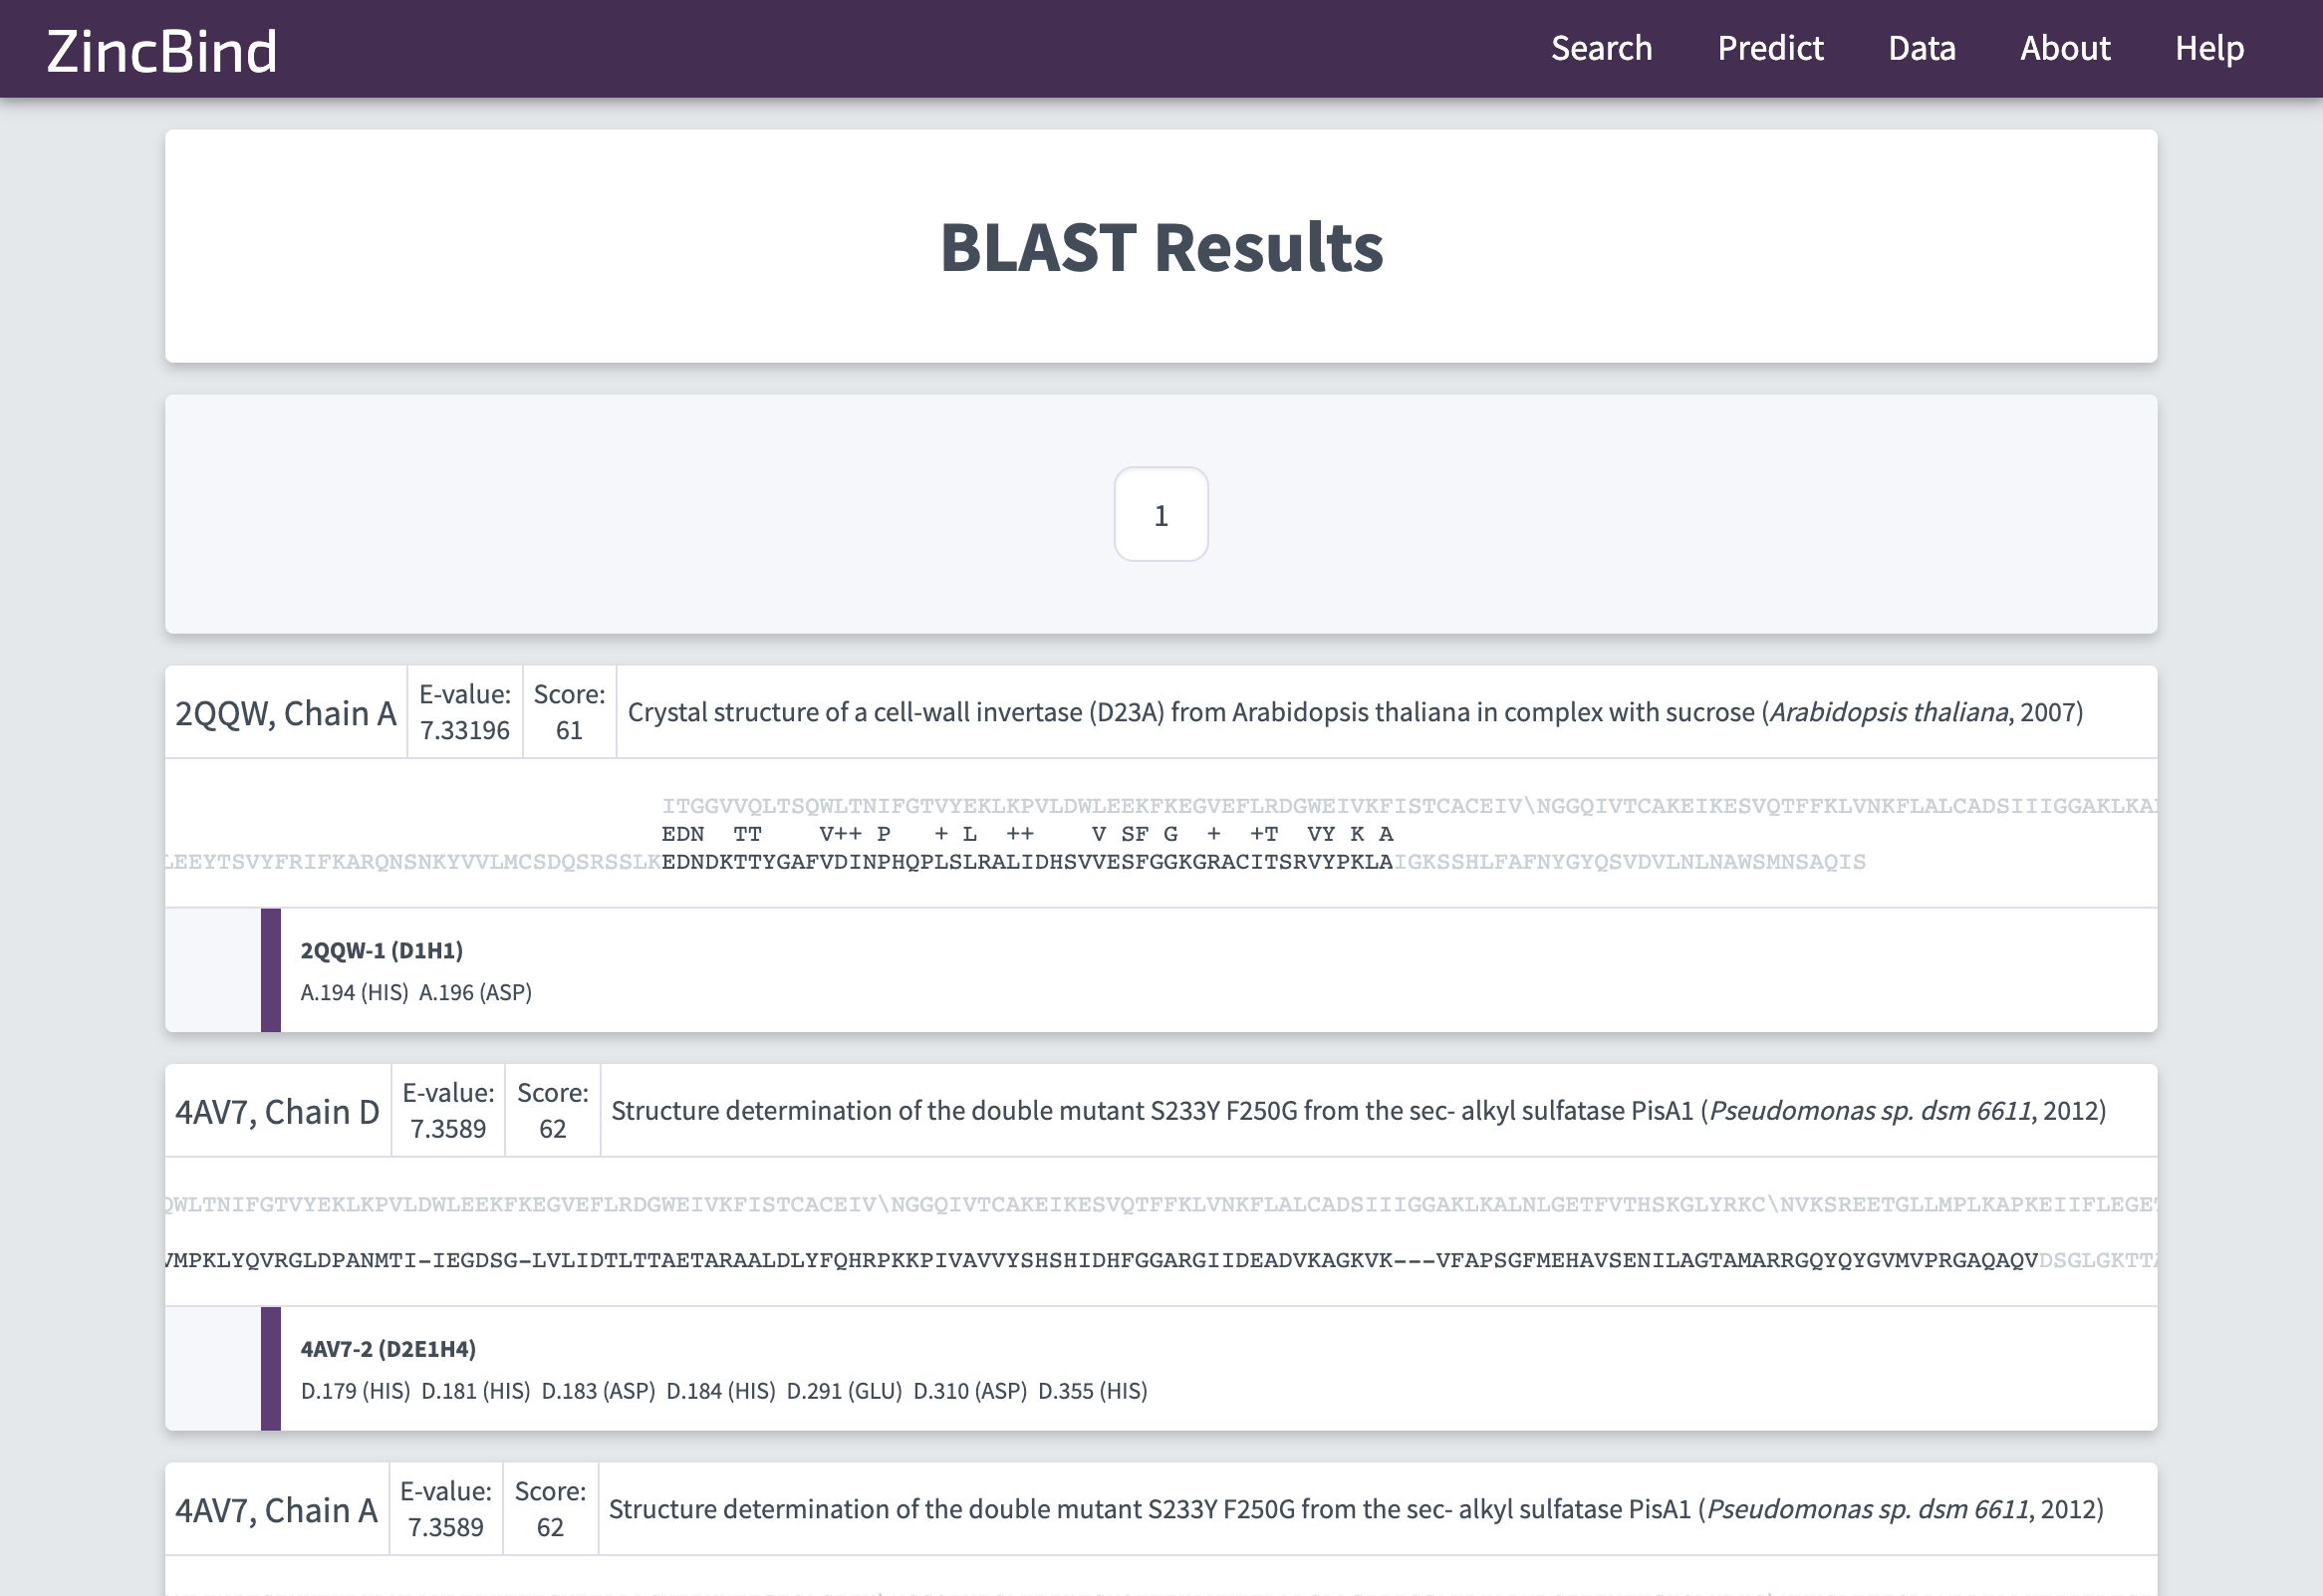
\includegraphics[width=1.0\textwidth]{Figures/zincbind-blast-results.eps}
\caption{\label{fig:zincbind-blast-results} An example of BLAST search results.}
\end{figure}

\begin{figure}
\centering
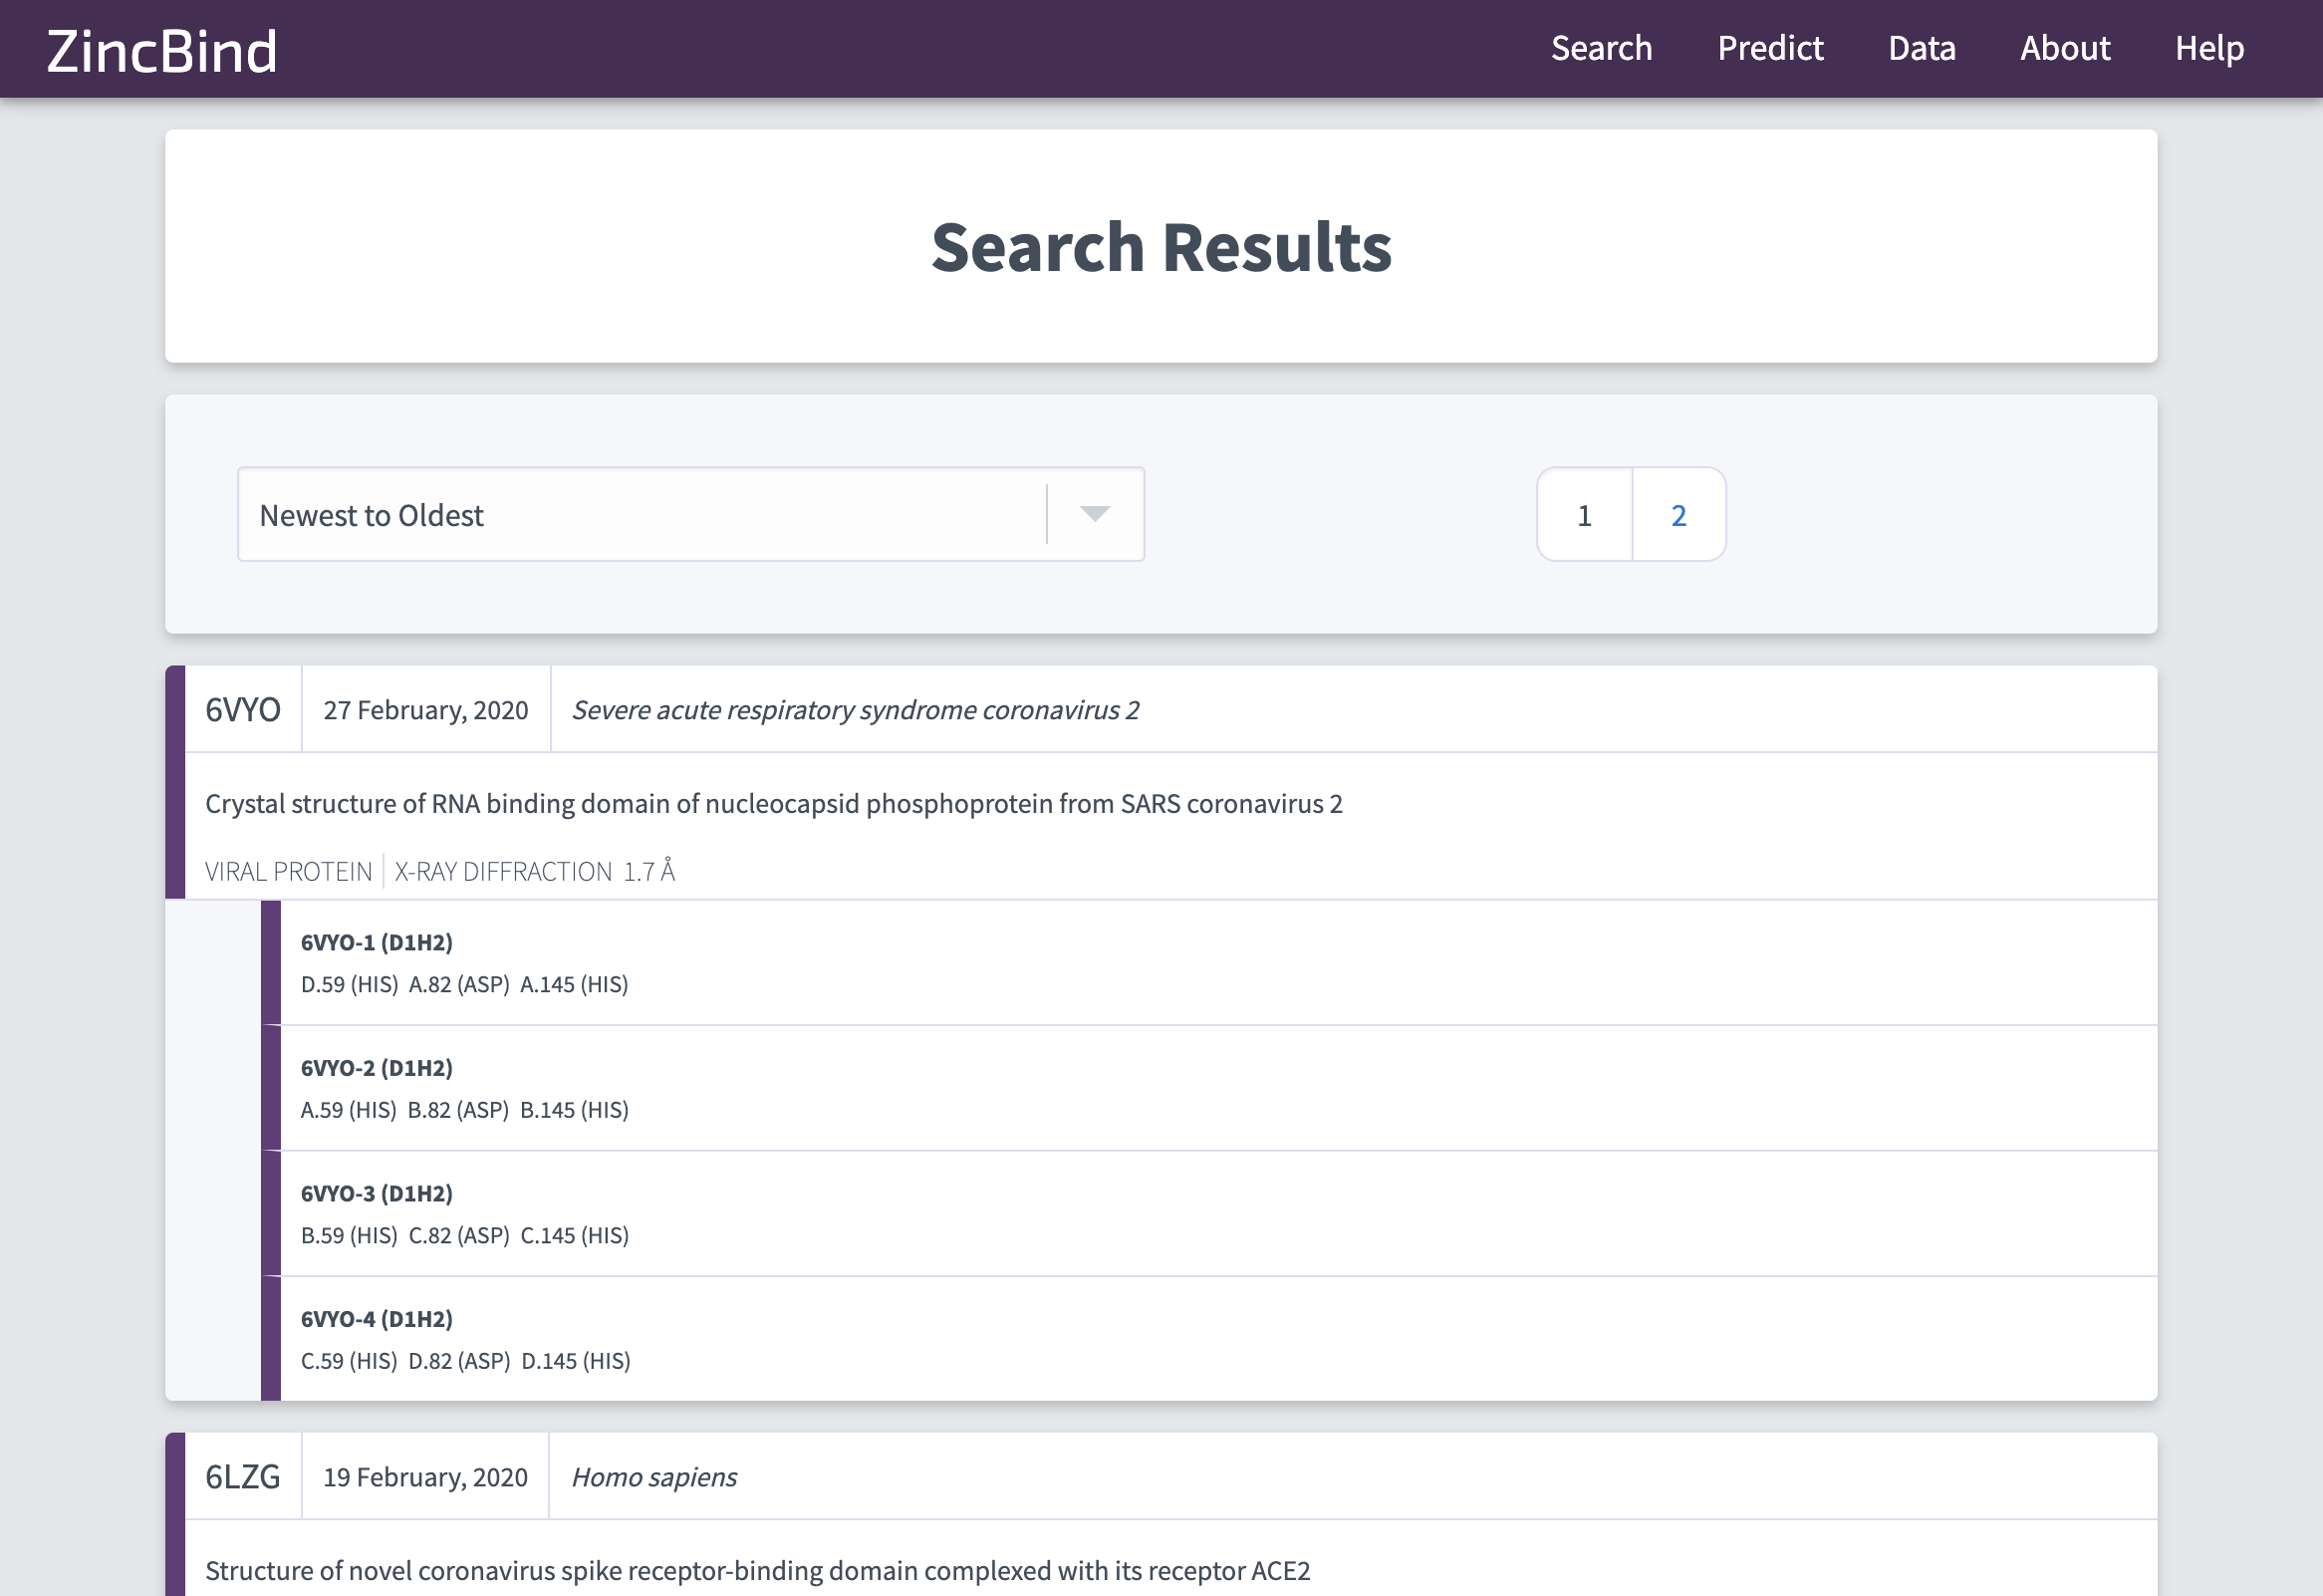
\includegraphics[width=1.0\textwidth]{Figures/zincbind-results.eps}
\caption{\label{fig:zincbind-results} An example of paginated (over two pages
in this case) search result showing matching PDBs, and the zinc binding sites
they contain.}
\end{figure}

PDB pages represent PDB records (see Figure ~\ref{fig:zincbind-pdb}). They provide basic information for that PDB (resolution, r-value, classification, source and expression organisms, experimental tehcnique, deposition date, and keywords --- the latter of which acts as a link to search by any of those keywords), as well as overviews of the zinc content of that PDB. The zincs associated with a binding site are listed as clickable links, while those without a binding site are listed along with their omission reason. Finally, there is a 3D manipulatable view of the PDB with all of its zinc binding sites. This uses the NGL JavaScript library, and beside it is a set of basic options for manipiulating the view, such as rotation options, background colour, and binding site highlighting --- this is in addition to NGL's built-in touch/drag/zoom manipulation. Generally the PDB page limits itself to information relevant to the structure's role as a zinc binding protein, but a link to the equivalent RCSB page is also provided for more information.

\begin{figure}
\centering
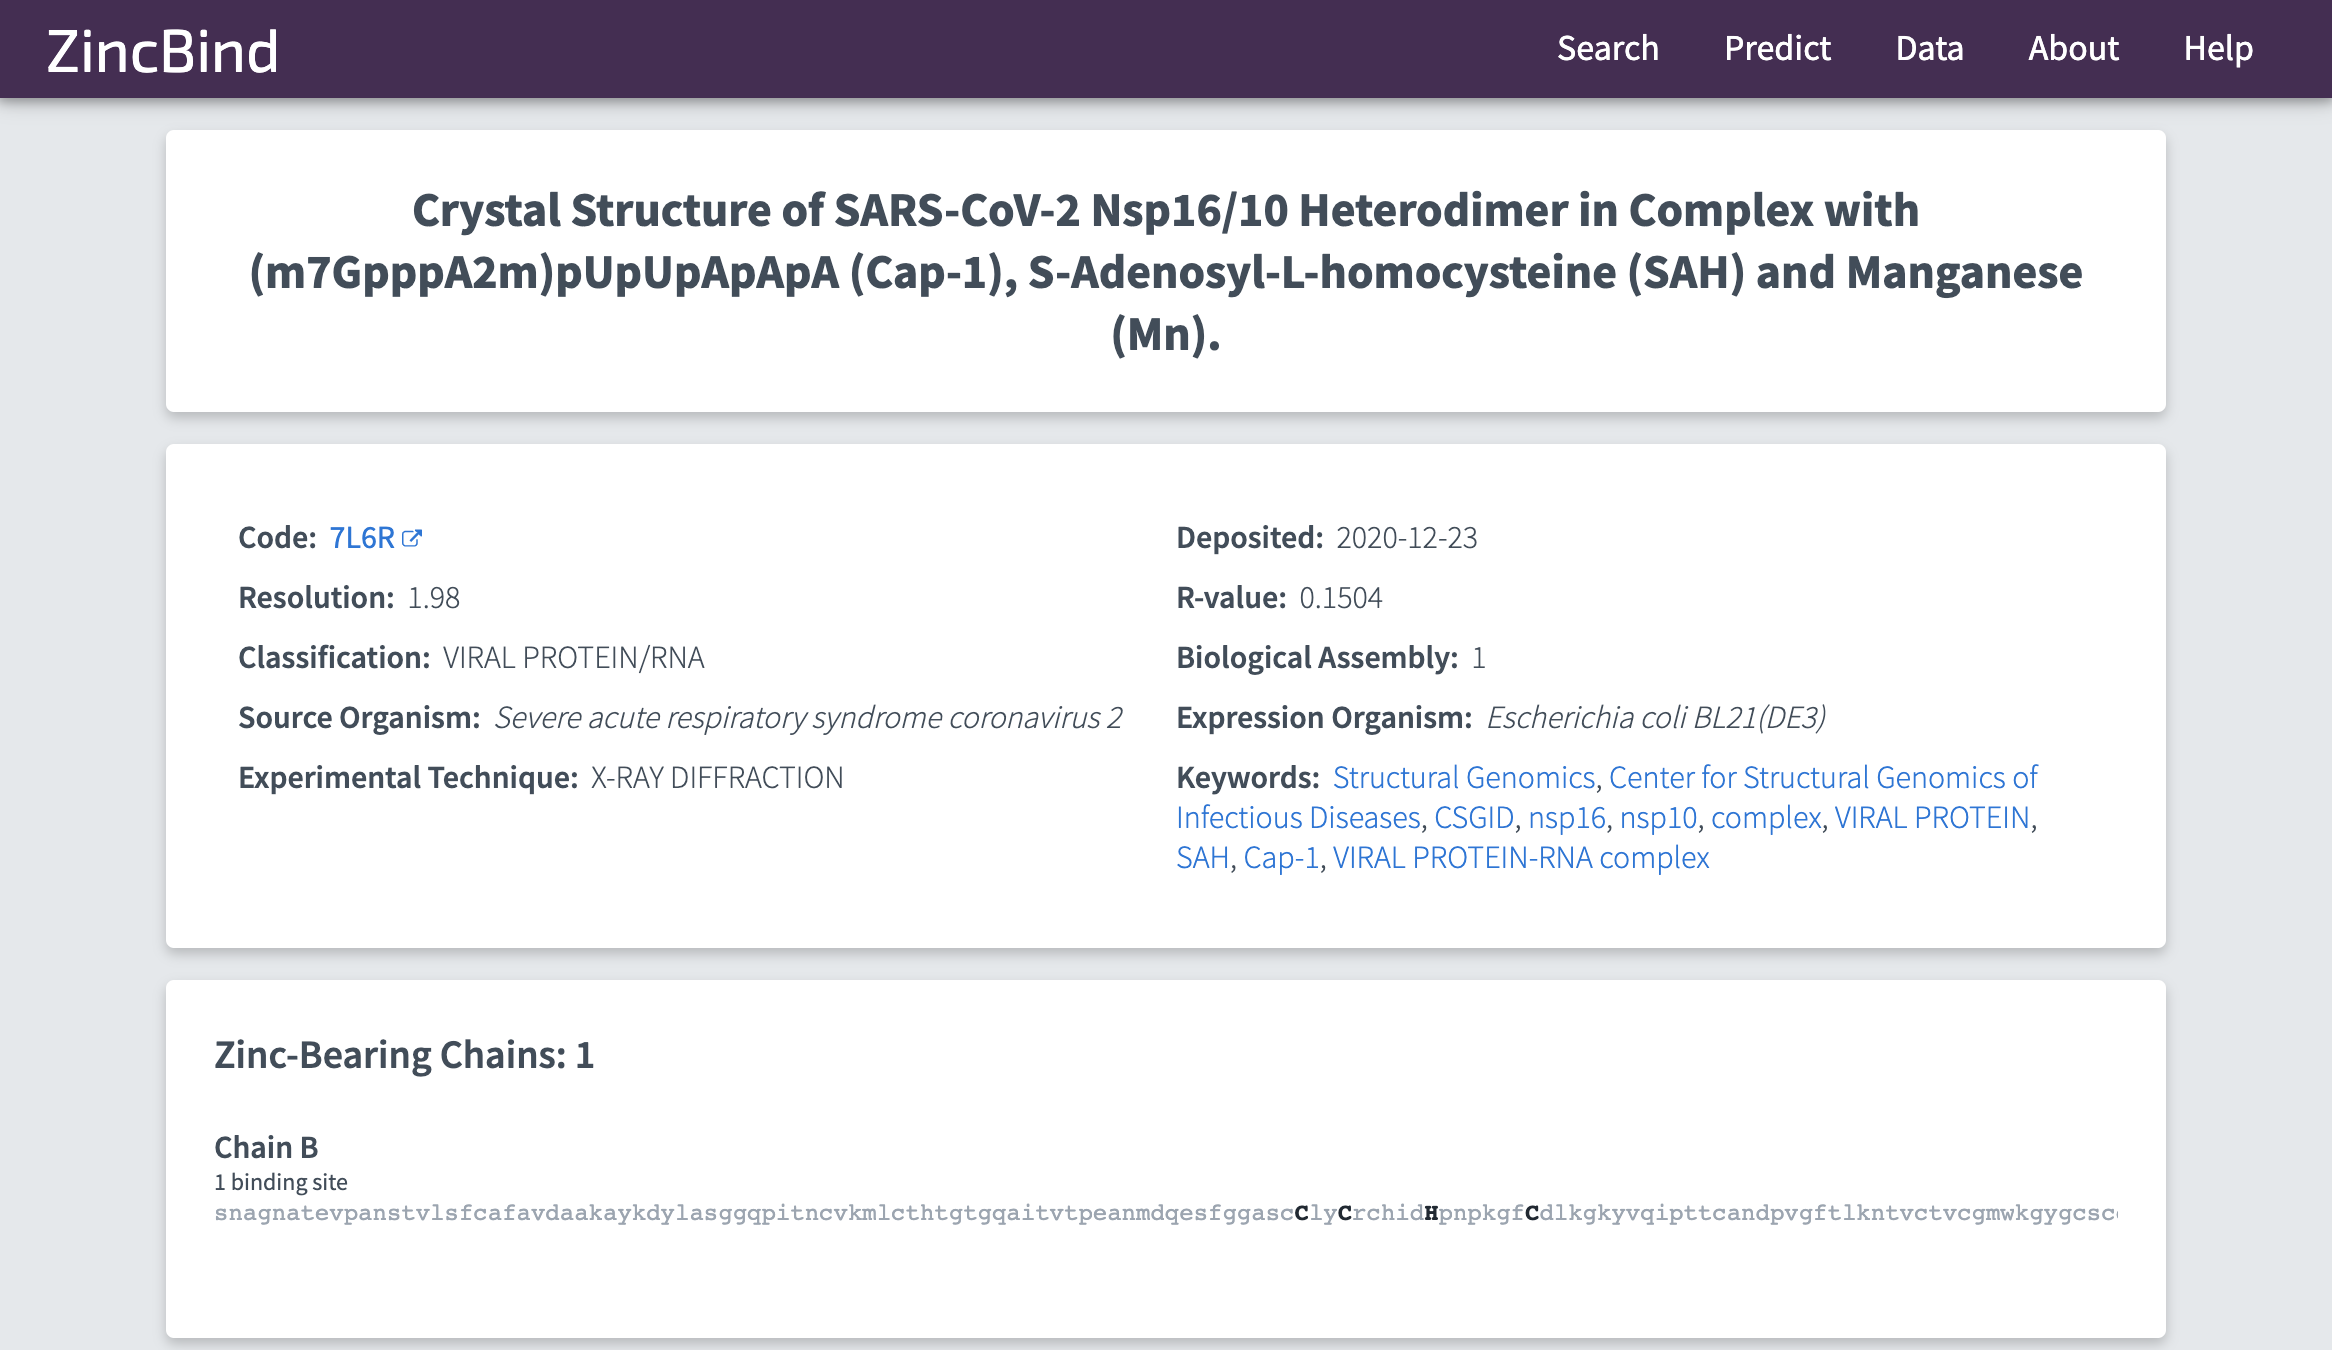
\includegraphics[width=1.0\textwidth]{Figures/zincbind-pdb.eps}
\caption{\label{fig:zincbind-pdb} An example of a PDB page in ZincBind, showing basic
information for that PDB. The three-dimensional structure view is further down the page.}
\end{figure}

The binding site pages (see Figure ~\ref{fig:zincbind-site}) contain more detail for that specific binding site, such as its mode of coordination, and links to equivalent sites in the same group. There is also a 3D manipulatable model of the binding site on this page --- this is broadly the same as that on the PDB page, except zoomed in to the specific site and with selectable individual residues and metals. The page also contains a summary of information for the containing PDB, and a link to that PDB's page.

\begin{figure}
\centering
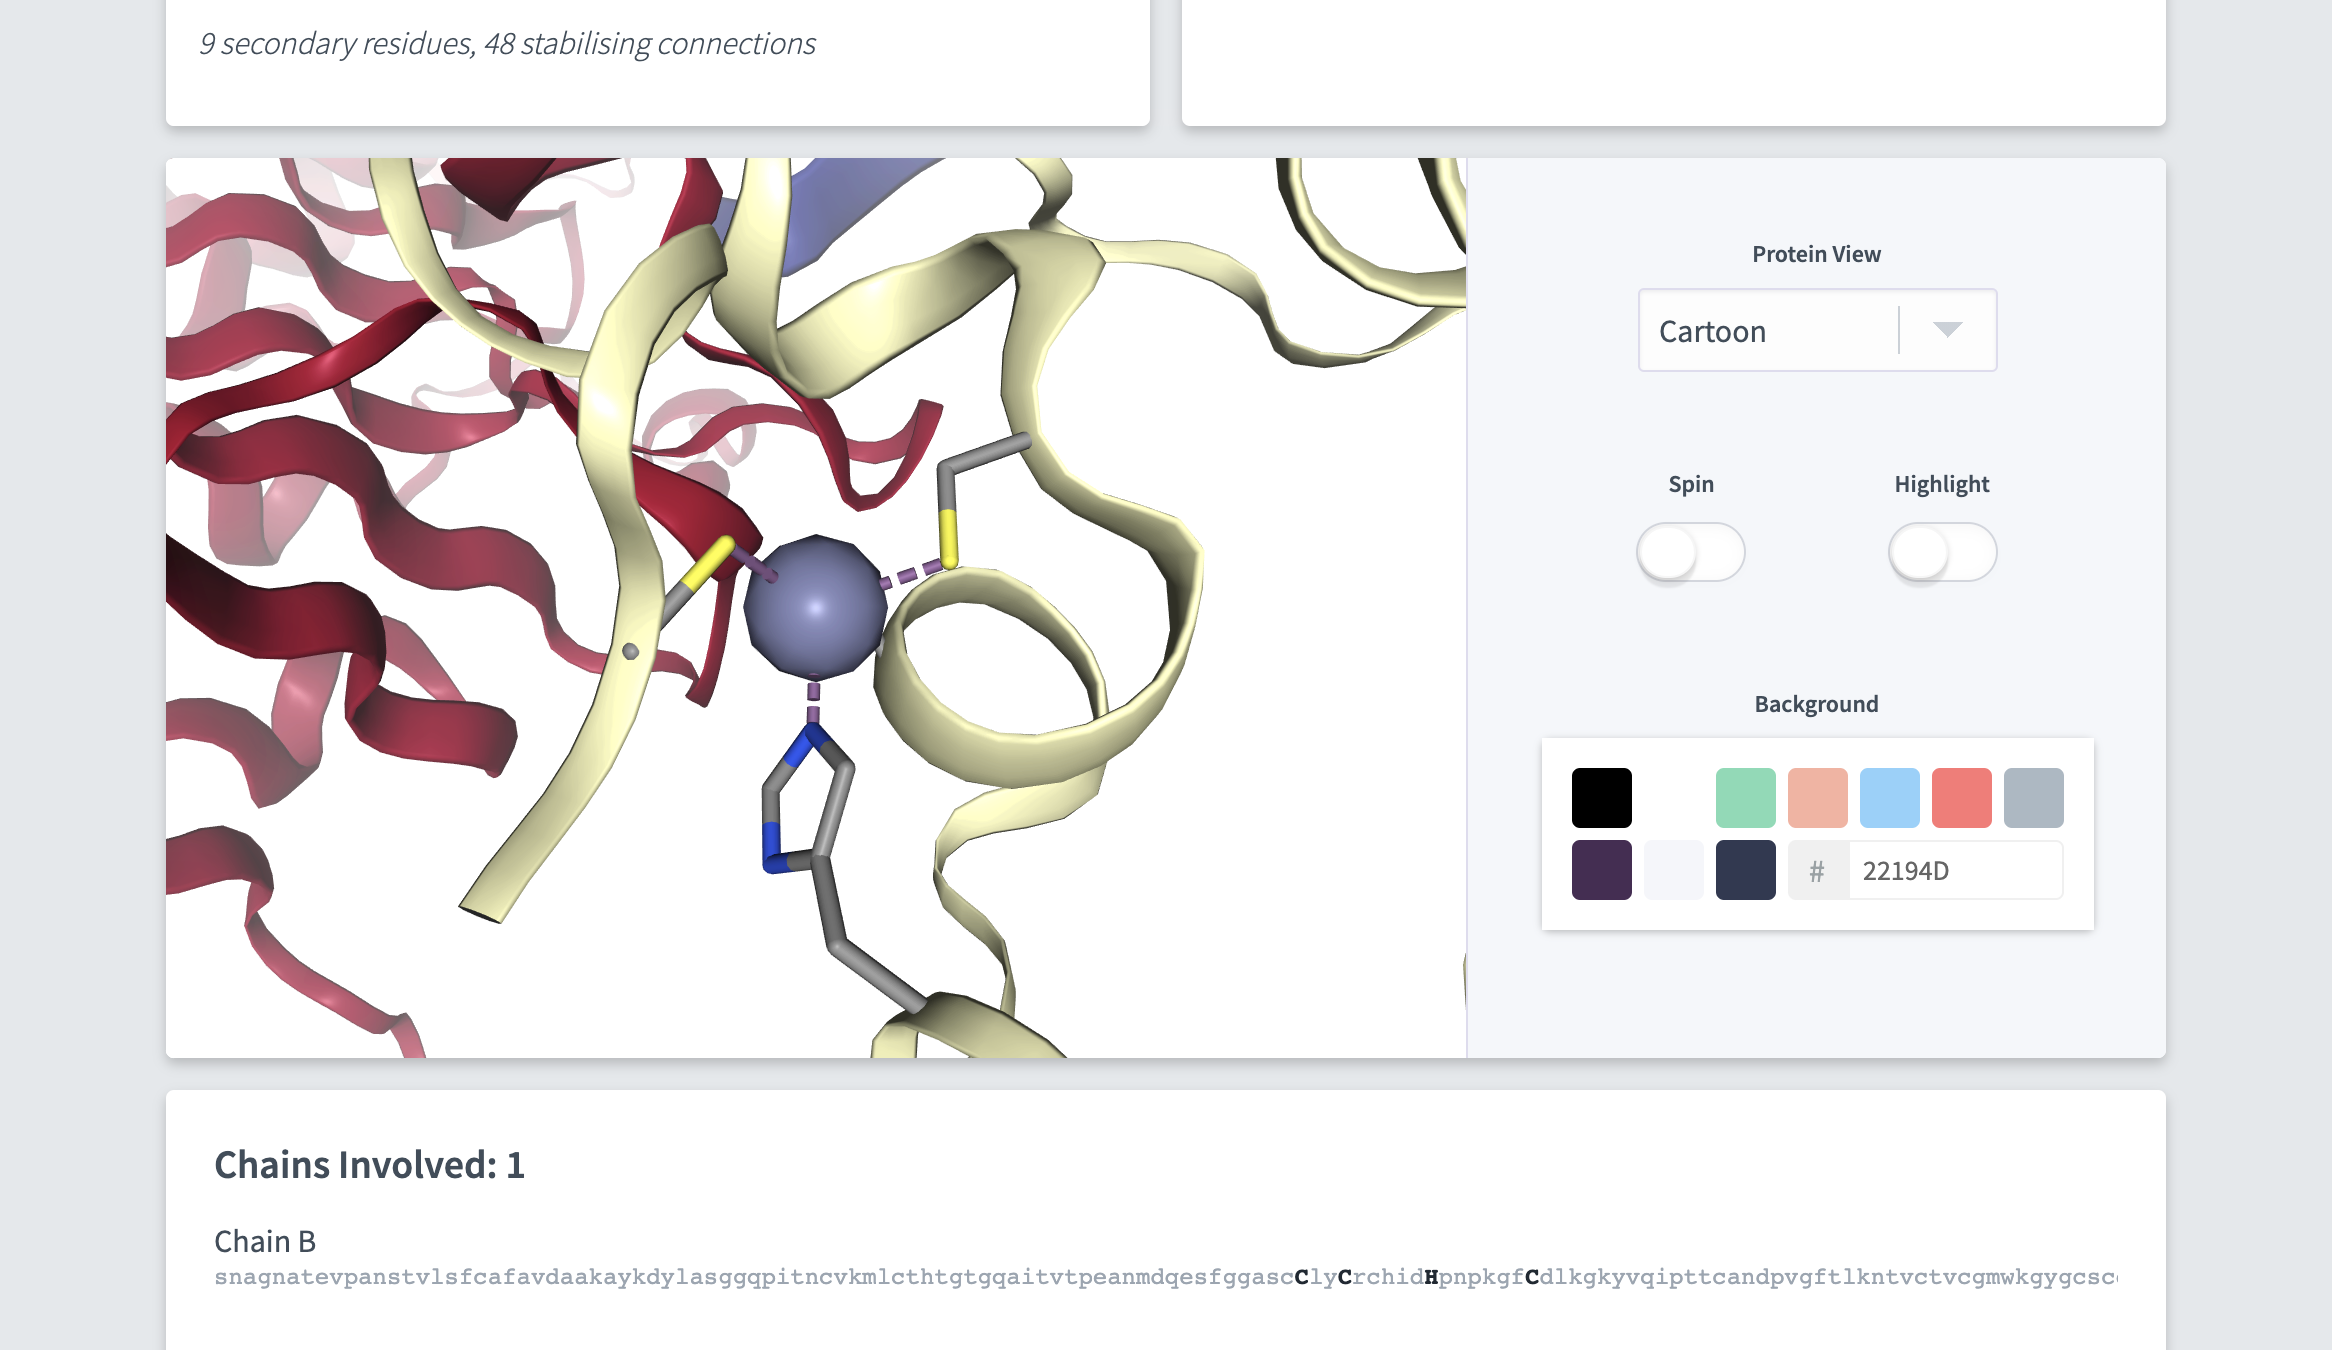
\includegraphics[width=1.0\textwidth]{Figures/zincbind-site.eps}
\caption{\label{fig:zincbind-site} An example of a binding site page in ZincBind, the manipulatable
3D NGL viewer, zoomed in to this binding site.}
\end{figure}

ZincBind also has a page that gives an overview of the dataset as a whole (see Figure ~\ref{fig:zincbind-data}). This contains charts for residue distribution, experimental methods, residue codes, resolution, species frequency, and PDB classification. These are intended to give a sense of the key properties of the database `at a glance'. There are also links to a page containing all data (essentially a modified version of the search results page that shows all PDBs, paginated), a link to an overview of the GraphQL API, and a link to a page showing how the sites are clustered into families and groups. Here each group lists the keywords and classifications that the sites in that group have in common to try and provide an automated way of annotating what the binding site the group represents actually does (see Figure ~\ref{fig:zincbind-group}).

\begin{figure}
\centering
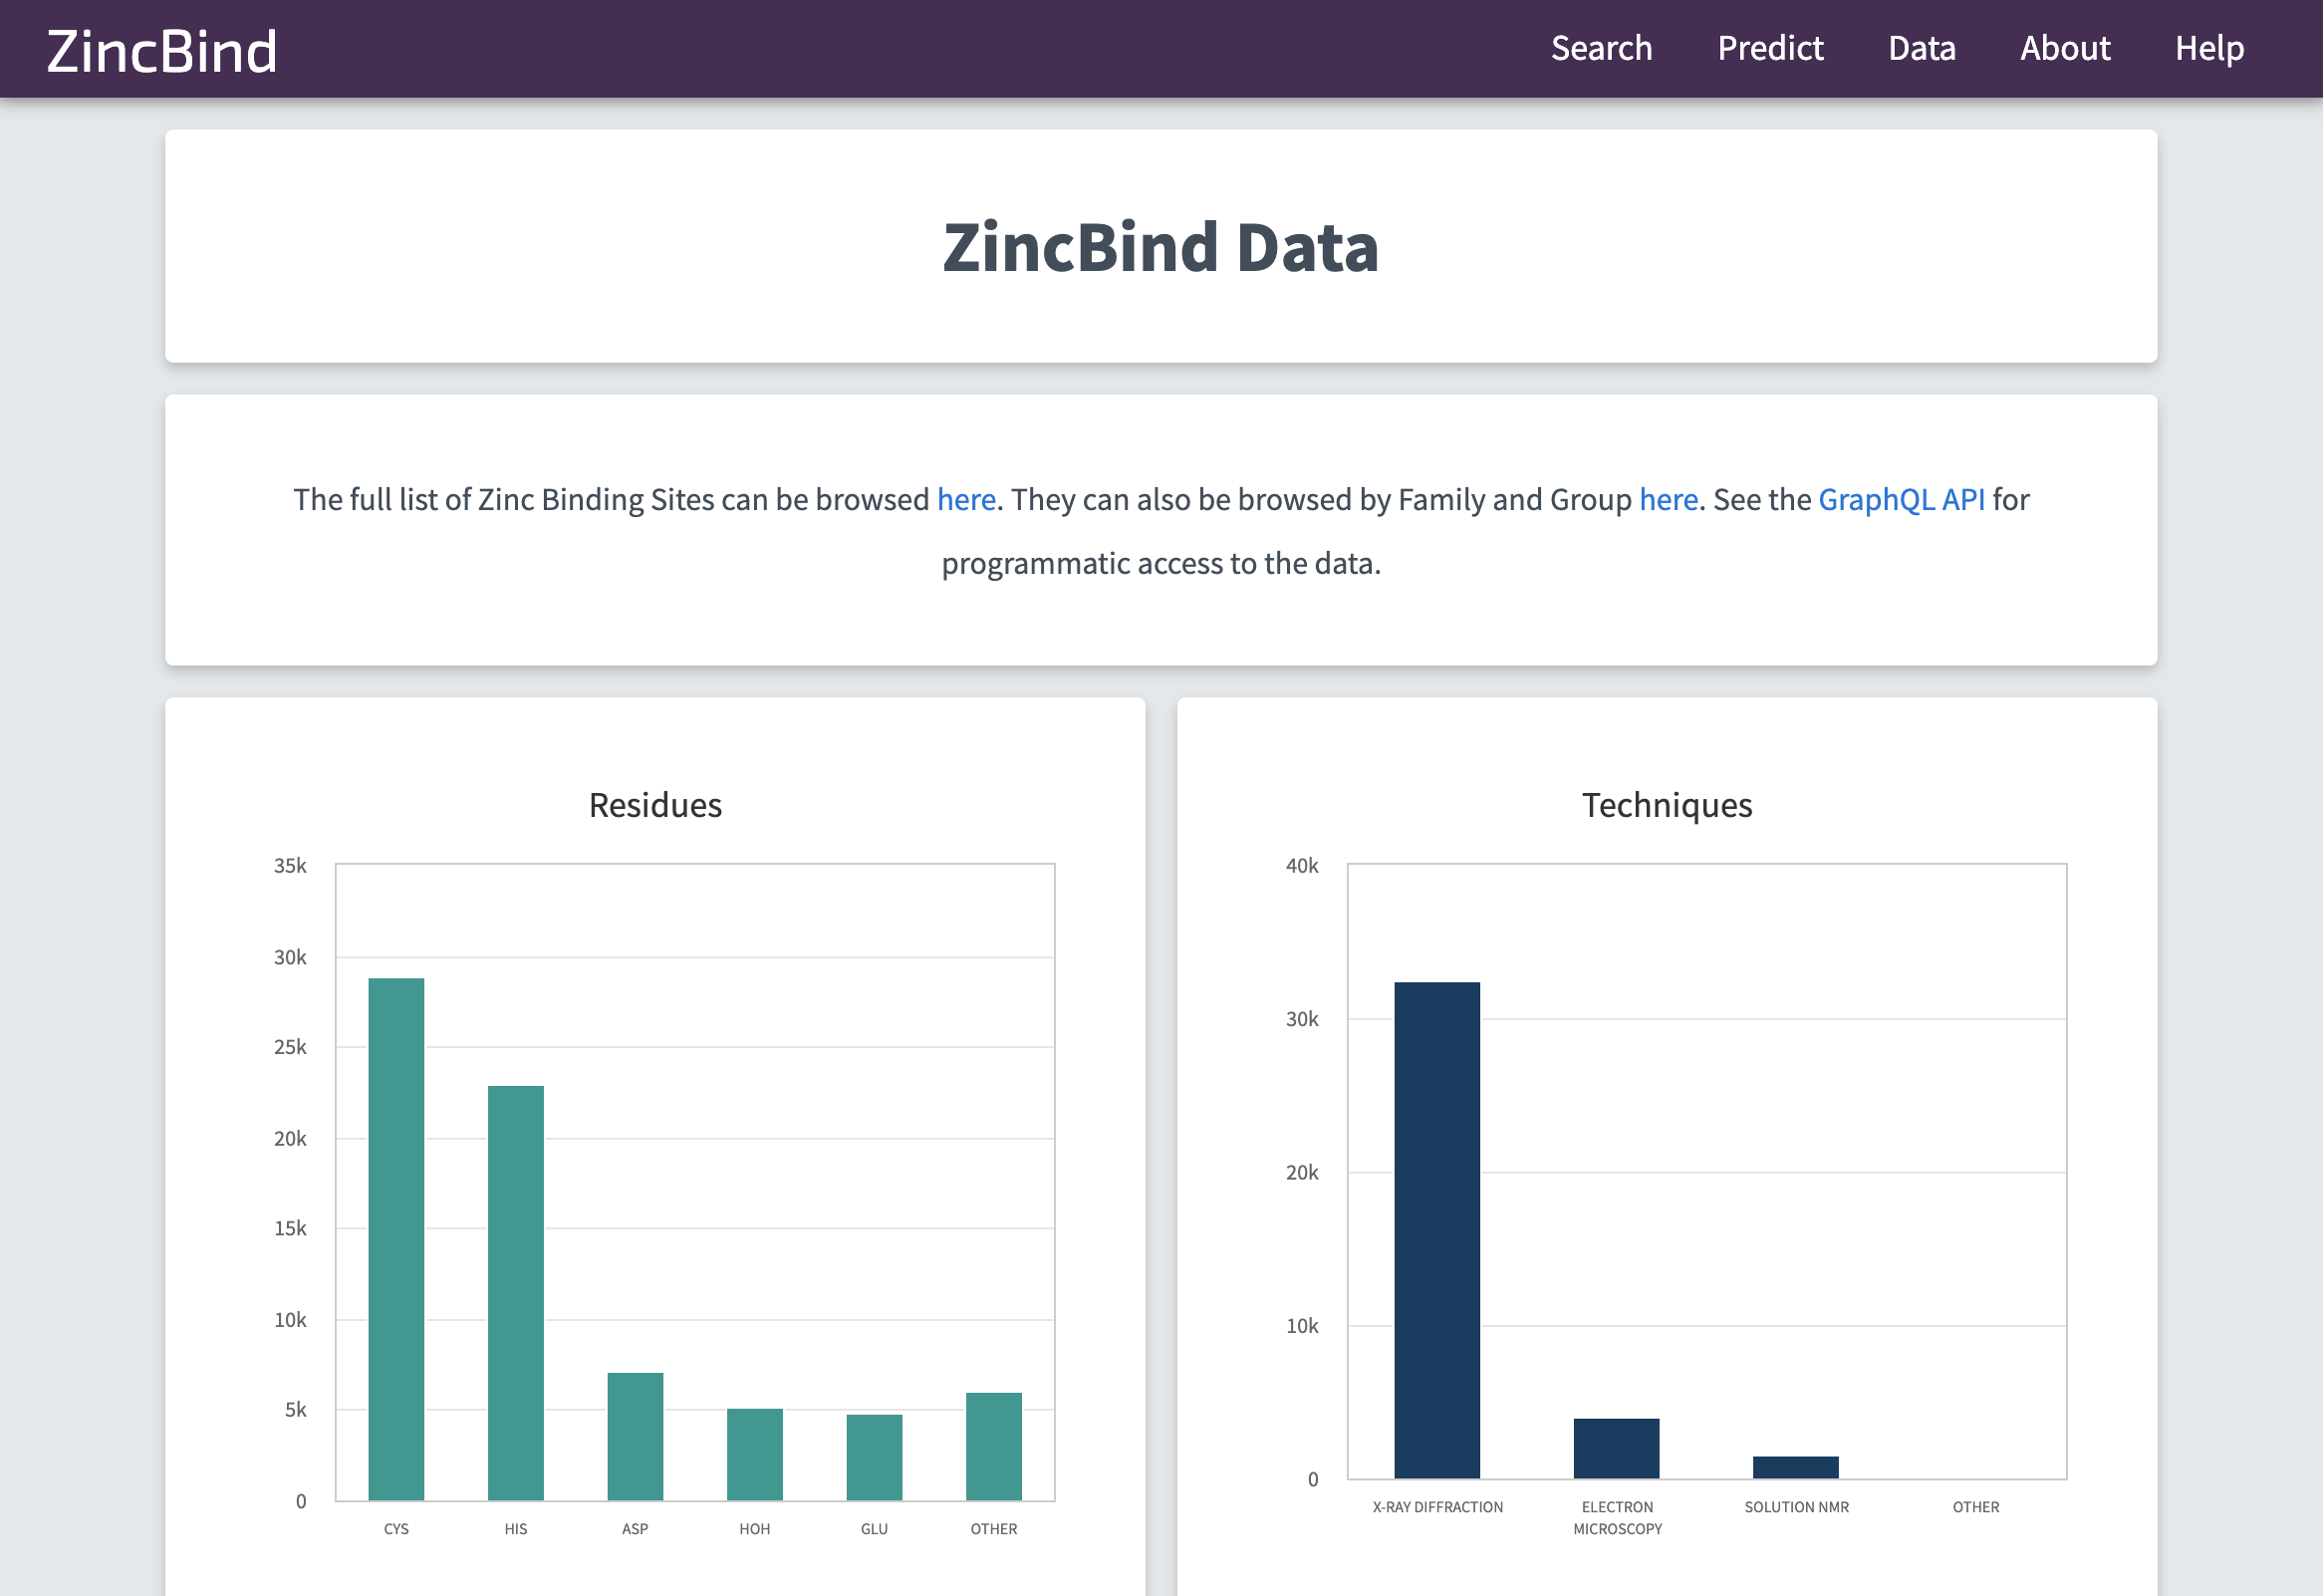
\includegraphics[width=1.0\textwidth]{Figures/zincbind-data.eps}
\caption{\label{fig:zincbind-data} Overview statistics for the dataset presented on
the ZincBind data page.}
\end{figure}

\begin{figure}
\centering
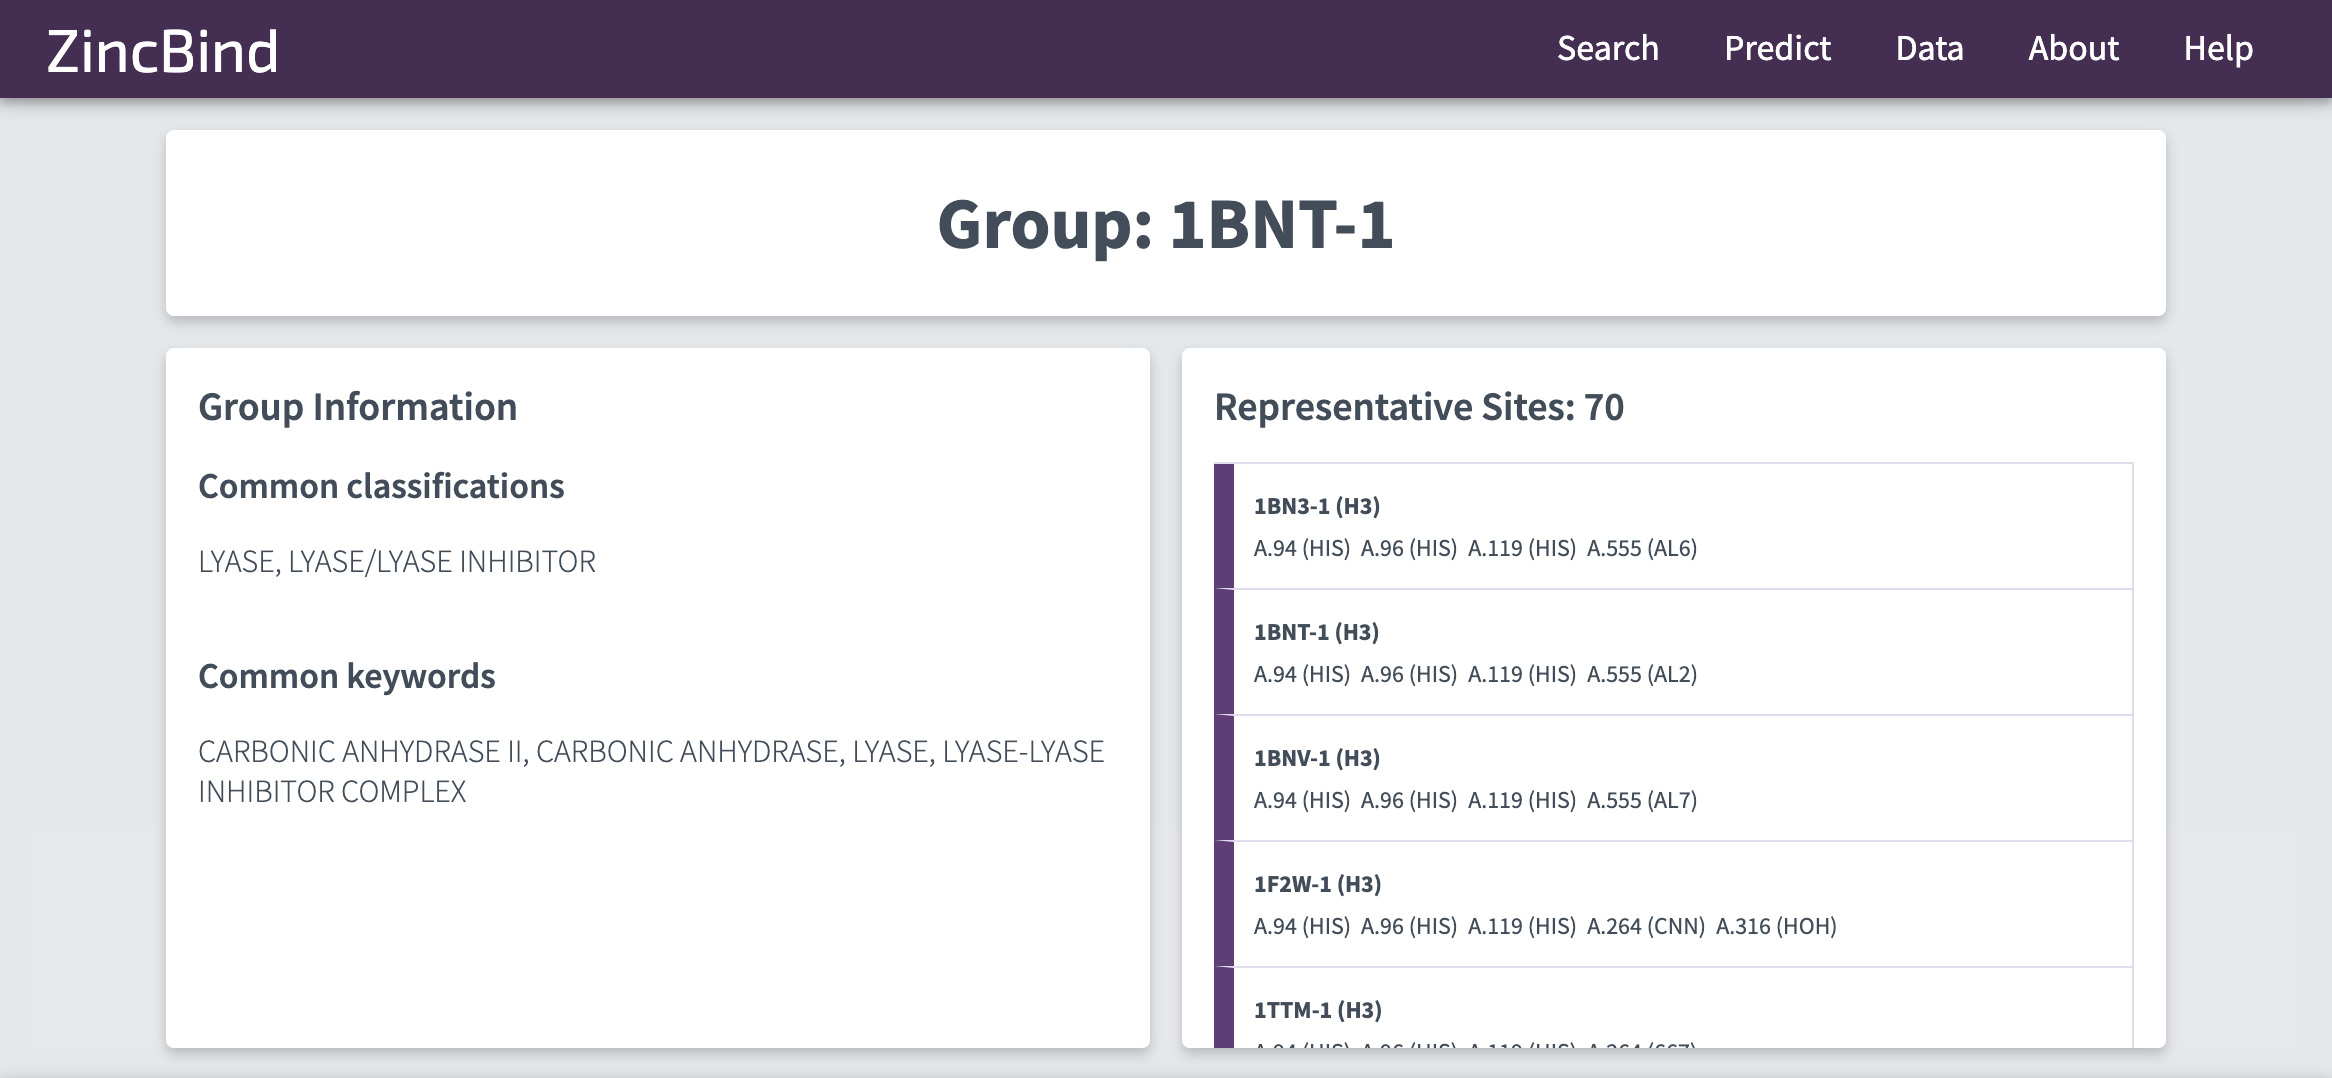
\includegraphics[width=1.0\textwidth]{Figures/zincbind-group.eps}
\caption{\label{fig:zincbind-group} A ZincBind group page, summarising the clustered zinc
binding sites and providing links to individual site pages.}
\end{figure}

There is a page dedicated to the prediction of binding sites that uses the seperate prediction API, but this will be covered in greater detail in the next chapter.

Finally, ZincBind has a help page, structured as a series of questions that a user may have.

Ultimately, the website is intended to serve as a way of broadening access to the database, which is continually updated. The API provides access to the data for researchers who need bulk access to the data, whereas the web frontend allows an individual to explore the data more casually to get a sense of what research might be carried out with it.

\section{Data Analysis}

The finished dataset offers a useful insight into the general properties of zinc binding sites - or at least, that subset of zinc binding sites for which structural information is available. Some of these properties are of use to building predictive models of zinc binding sites, whereas others are of more general interest. An overview of the main findings that can be gleaned from the dataset will be presented here. All values are correct at the time of writing ({\today}), though as this is a continually and automatically updated dataset, the precise values will vary slightly as time goes on. It is not anticipated that these changes will alter the overall conclusions, as the dataset is very large already.

\emph{Note that much of this text has previously appeared in the ZincBind publication from January 2019, though the values have been updated for the updated dataset.}

\subsection{The Prevalence of Zinc}

Of the 174,014 PDB structures in the Protein Data Bank at the time of the most recent database update, 17,556 contained at least one zinc atom and are accounted for in ZincBind. This porportion - 10.1\% - is very close to the 10\% of human proteins usually said to contain zinc, though as the Data Bank does not purport to be representative sampling of any genome, human or otherwise, there was no particular reason for this to be the case.

\subsection{Qualifying Atoms}

In total, when run in January 2021, ZincBind identifies 65,595 zinc atoms and 1,138 other metal atoms associated with zinc atoms when searching the raw coordinates of the PDB asymmetric units. Other metals are only stored in ZincBind if they are part of a multi-metal binding site with at least one zinc atom, so the vast majority of metals in the database are zinc. Of the non-zinc metals, the most common of these `co-active' metals are magnesium, potassium, iron and copper.

Of the 65,595 zinc atoms in the database, 24,246 (37.0\%) are not associated with any binding site, and are in the database solely to acknowledge their existence. The most common reason for not assigning a zinc atom to a binding site is that the atom is duplicated multiple times in the asymmetric unit, but appears only once in the biological assembly used for processing - 13,124 metals were excluded for this reason. For example, PDB entry 1A4L contains four chains, each with one zinc atom, but the biological assembly only uses one. The other three are stored in ZincBind with an omission reason, but have no binding site assigned to them. Figure ~\ref{fig:omission} shows the breakdown of zinc atoms by omission reason.

Using the full biological assembly leads to zinc ions being both excluded, and included as being associated with binding sites. As stated above, it is common for the asymmetric unit of a PDB file to contain multiple copies of the biomolecule of interest as a result of crystallization, but once the `correct' assembly is chosen, these duplicated zinc atoms will be absent from the final structure. Conversely, using the full biological assembly rather than just the raw asymmetric unit coordinates of the PDB is crucial when the zinc atom is present at an interface between chains. In the asymmetric unit, there may be a single residue coordinating with the ion - if symmetry were not considered, such a model would be discarded by the ZincBind algorithm as a salt.

\begin{figure}
\centering
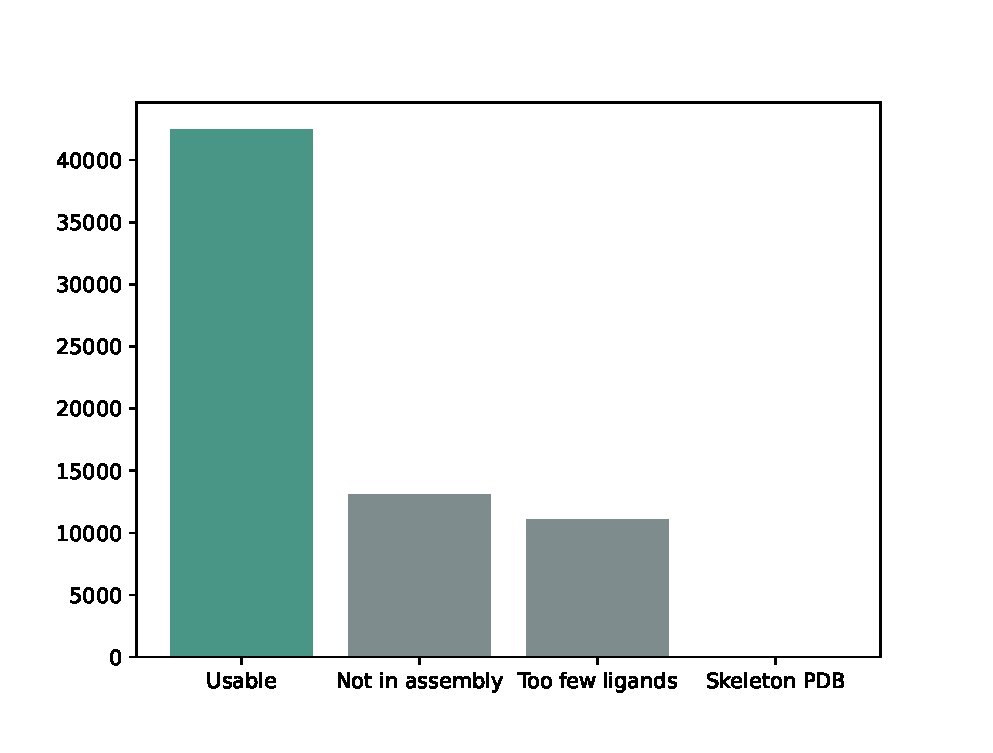
\includegraphics[width=1.0\textwidth]{Figures/omission.eps}
\caption{\label{fig:omission} Illustrating the relative frequency of omission reasons for zinc
atoms that were ultimately not assigned to a binding site. There were 8 which were omitted because
the PDB structure did not contain side chains --- insignificant compared with the other two reasons.}
\end{figure}

\subsection{Zinc Binding Sites with High Representation}

The 42,487 metal atoms, for which binding site information is stored, are part of a total of 38,035 zinc binding sites in ZincBind. After clustering the proteins at 90\% sequence identity and then clustering the binding sites as described above, there are 17,471 unique zinc binding sites in the database. The binding site with the most copies is from carbonic anhydrase (355 copies), a catalytic serum protein and, as already noted, the first known zinc binding protein. This is followed by JMJD2D (247 copies), a lysine-specific demethylase. 11,785 (67.5\%) zinc binding sites are currently unique in that they have only one structure, and are therefore only represented once in ZincBind. The initial distribution is shown in Figure ~\ref{fig:group-clusters}

\begin{figure}
\centering
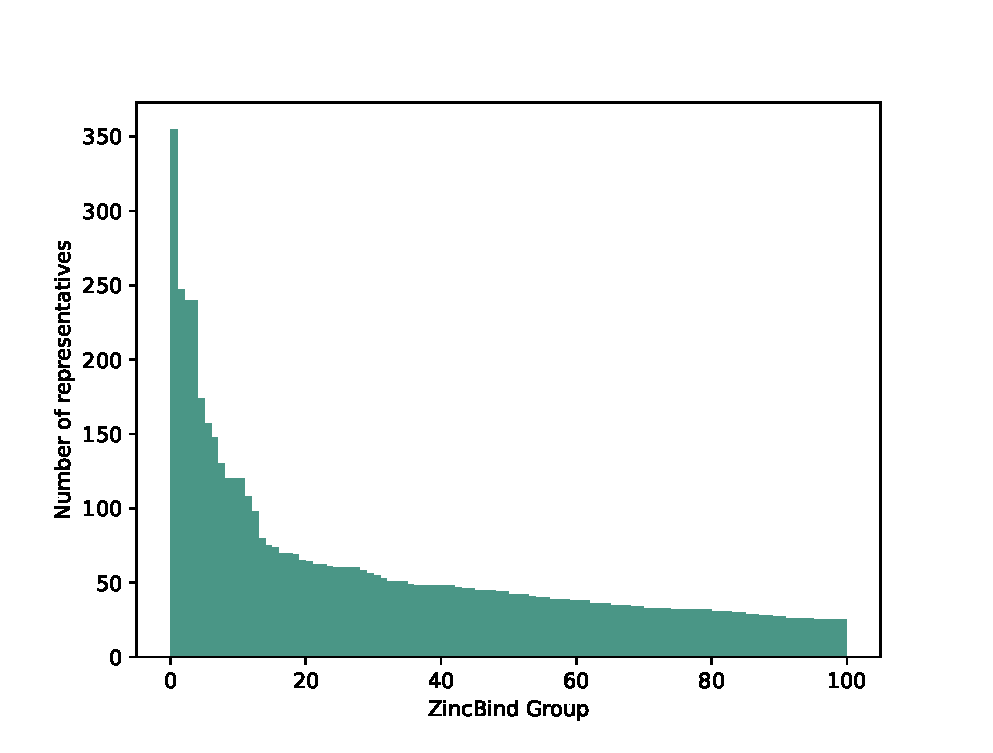
\includegraphics[width=1.0\textwidth]{Figures/group-clusters.eps}
\caption{\label{fig:group-clusters.eps} The distribution of binding sites among groups for the hundred most populated groups.}
\end{figure}

For each cluster of equivalent zinc binding sites, the best resolution structure is chosen to provide a single site which is flagged as the `representative' for that cluster.

\subsection{Liganding Residues}

The binding residues that dominate zinc binding sites are well established: cysteine, histidine, and the acidic residues aspartate and glutamate. This is supported by the data in ZincBind. There are a total of 161,324 liganding residues in ZincBind, of which those four residue types, together with water, comprise 93.0\% of all zinc-liganding residues. Note, however, that this considers every binding site in the database. When non-redundant sites are studied (i.e.\ only one site per cluster thereby removing the bias towards more intensely studied proteins), these five comprise a slightly smaller percentage of zinc-liganding residues (92.0\%). This suggests that the binding sites most frequently appearing in the PDB show slightly less variation than a more representative sampling.

The secondary residues, those which contact the primary liganding residues, are also stored in ZincBind and here there is more variation. The most common secondary residue is Glyceine (9.1/%), followed by leucine (7.4\%) and alanine (7.2\%). Broadly speaking, hydrophobic residues tend to be slightly more predominant than hydrophilic residues, which can be seen when the twnety amino acids' hydrophobicities are plotted against their frequency, which shows a correlation coefficient of 0.34 --- a weak but significant link (see Figure ~\ref{fig:secondary-residues}).

\begin{figure}
\centering
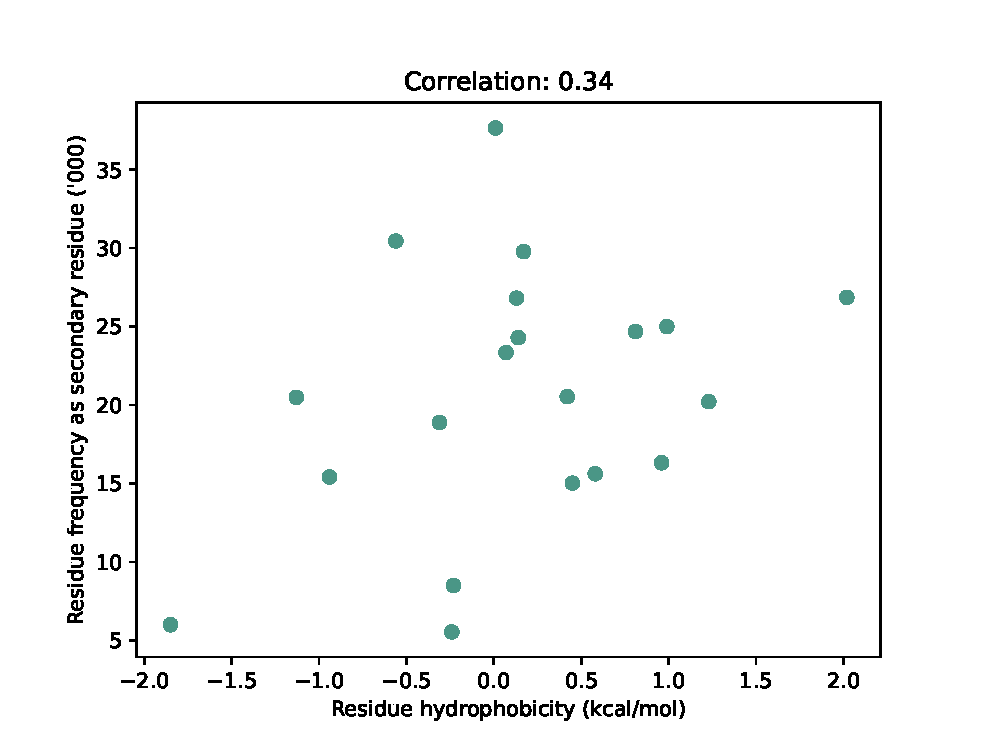
\includegraphics[width=1.0\textwidth]{Figures/secondary-residues.eps}
\caption{\label{fig:secondary-residues.eps} There is a weak correlation between residue hydrophobicity and their frequency as a secondary residue in zinc binding sites.}
\end{figure}

If the primary binding residues' single letter codes are combined to give an overall `signature' of the binding site, C4 (four cysteine residues) is the most prevalent, with 3,069 of the 17,471 unique binding sites having this arrangement of residues (17.6\%) - followed closely by C3H1, with 2149 (12.3\%). That the most common signature makes up just 17.6\% of the total is indicative of the relatively high diversity in such signatures. Between them, the top ten residue signatures account for just 64.4\% of the total.

Of the 24,200 redundant binding sites that contain just one zinc atom, and which come from structures with resolutions better than 3\AA, the most common mode of coordination is via four liganding atoms: 15,077 examples (62.3\%). 5-coordination and 3-coordination have similar prevalences: 4504 (18.6\%) and 1840 (7.6\%) respectively. It is likely that 3-coordination is being over-represented here as in practice many sites which have three liganding atoms in the PDB structure are likely missing a fourth ligand in the form of water, meaning that tetrahedral geometry is probably even more widespread than suggested here.

This same subset of binding sites can be used to investigate liganding atom distances. Nitrogen and sulphur atoms both have characteristic distances with tight distributions: $2.12\pm0.16$\AA\ and $2.34\pm0.12$\AA\ respectively. Oxygen however as a much wider distribution, as it can be provided by either of the carboxylate oxygens of the acidic side chains, or from water, with the angle of these two atoms varying continuously. Its average distance to zinc is $2.29\pm0.22$\AA. Overall the average metal-ligand distance is $2.25\pm0.24$\AA (see Figure ~\ref{fig:atom-distances})

\begin{figure}
\centering
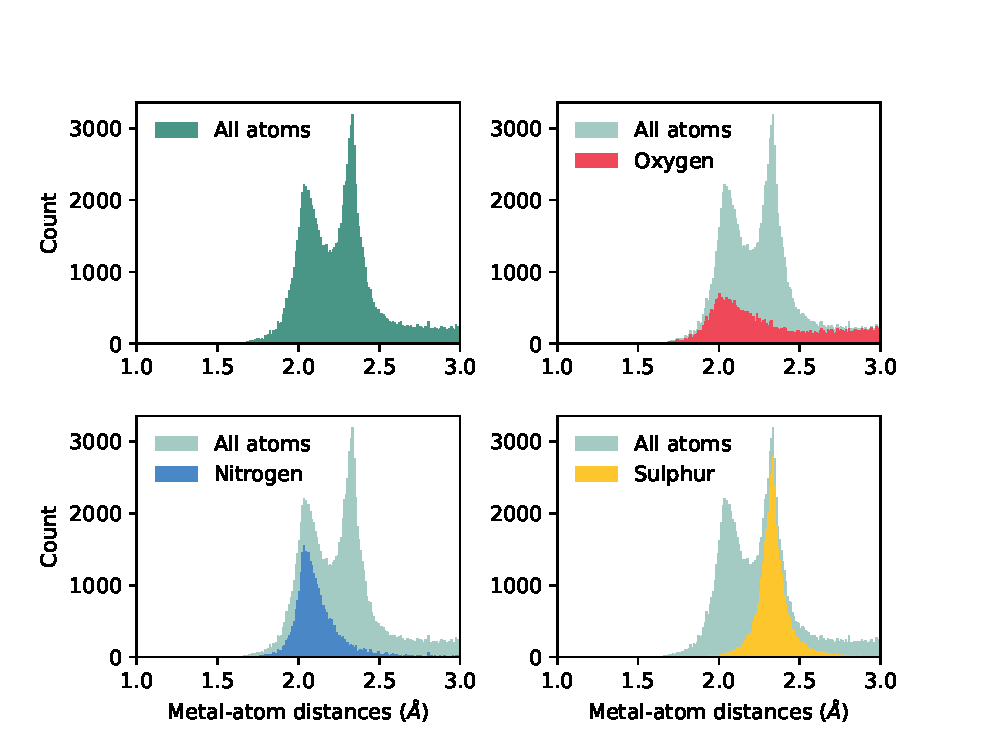
\includegraphics[width=1.0\textwidth]{Figures/atom-distances.eps}
\caption{\label{fig:atom-distances.eps} The distribution of liganding atom
  distances in all single-zinc sites, with a resolution better than
  3\AA. The overall distribution can be seen as bimodal, with the
  first peak being the preferred distance of nitrogen and oxygen, and
  the second peak being the preferred distance of sulphur, which has a
  greater Van der Waals radius.  While nitrogen and sulphur both have
  tight distributions, oxygen does not, and has a much more prominent
  tail in its distribution.}
\end{figure}

\subsection{Co-active Binding Sites}

In some cases multiple metals act in concert to form a single functional unit. Such sites are generally referred to as co-active binding sites in the literature (or `co-catalytic' where the site is known to have a catalytic function). Here, such sites are defined as those instances where a single residue is liganded to more than one metal, according to the criteria defined above. The metals are organised into a single site as described in the methods.

In ZincBind, 3976 from the total of 38,035 zinc binding sites (12.7\%) contain multiple metals - 3550 contain two metals, 394 contain three, 22 contain four, two contain five, and eight zinc binding sites contain six metals - though two of these are from a synthetic construct. In some cases these are binding sites with multiple zinc atoms, but in others the zinc is acting in concert with other metals. Potassium is the most common, represented 319 times, followed by iron (188) and copper (155).

These multi-metal sites account for all of the non-zinc metals in the ZincBind database. While the term `co-catalytic' is sometimes used interchangeably with `co-active', only 83.6\% are derived from an enzymatic protein (defined here as a protein name ending in \emph{--ase}). However this compares with just 61.1\% of all zinc-only binding sites that are enzymatic. A Fisher exact test showed the difference to be significant ($p<0.00001$).

\section{Conclusion}

ZincBind is a database of zinc binding sites --- as such it is both a valuable dataset for this PhD, in the sense that it will serve as training data for predictive models of zinc binding (see next chapter), but it is also a useful resource in its own right. It is is publicly accessible, with a modern GraphQL API and responsive website providing access to the data. The data themselves are continuously and automatically updated, and have charactersitics broadly in line with previously observed properties of zinc and other metal binding sites in previous, smaller datasets.

The remainder of this thesis will focus on the dataset's role as a training set for predictive models.
%%%% MACRO DEFINITION %%%%

\providecommand{\pvivax}{P.~vivax}
\providecommand{\pfalciparum}{P.~falciparum}
\providecommand{\cterm}{C-terminus}
\providecommand{\nterm}{N-terminus}

\providecommand{\e}[1]{\ensuremath{\times 10^{#1}}}
\newcolumntype{P}[1]{>{\centering\arraybackslash}p{#1}}
\newcolumntype{M}[1]{>{\centering\arraybackslash}m{#1}}

\providecommand{\refimage}[1]{\figurename~\ref{fig:#1}}

%TC:macro \note [ignore]



%%%%%%%%%%%%%%%%%%%%%%%%%%%%%%%%%%%%%%%%%%%%%%%%%%%%%%%%%%%%%%%%%%%%%%%%%%%%%%%%%%%%%%%%%%%%%%%%%%%%%%%%%%%%%%%%%%%%%
%%%%%%%%%%%%%%%%%%%%%%%%%%%%%%%%%%%%%%%%%%%%%%%%%%%%%%%%%%%%%%%%%%%%%%%%%%%%%%%%%%%%%%%%%%%%%%%%%%%%%%%%%%%%%%%%%%%%%
%													BEGIN
%%%%%%%%%%%%%%%%%%%%%%%%%%%%%%%%%%%%%%%%%%%%%%%%%%%%%%%%%%%%%%%%%%%%%%%%%%%%%%%%%%%%%%%%%%%%%%%%%%%%%%%%%%%%%%%%%%%%%
%%%%%%%%%%%%%%%%%%%%%%%%%%%%%%%%%%%%%%%%%%%%%%%%%%%%%%%%%%%%%%%%%%%%%%%%%%%%%%%%%%%%%%%%%%%%%%%%%%%%%%%%%%%%%%%%%%%%%

\chapter{Predicting Zinc Binding Sites} % Write in your own chapter title
\label{Chapter4}
\lhead{Chapter 4. \emph{Predicting Zinc Binding in Proteins}} % Write in your own chapter title to set the page header

The aim of this part of the PhD is to create a system which conceptually is quite simple --- it would take as its input a protein sequence or protein sequence, and output a list of zero or more residue combinations which are predicted to form a zinc binding site, with an accompanying probability.

This system is a machine learning system - it uses binary classifiers trained on the large dataset of zinc binding sites described in the previous chapter which `learn' what zinc binding sites look like from that data.

This chapter will describe the approach taken to solving this problem, the models created, the architecture of the system from the user's point of view, and how the models are accessed and used.

\section{Approach}

As explored in Chapter 2, there have been multiple studies in the past which have used machine learning (or simpler methods) to create zinc-binding predictors (or general-purpose metal-binding predictors). Many of the general principles of these studies are adopted here, however there are two crucial methodological changes that I have chosen to make.

One recurring feature of these previous works, particularly in the sequence-based predictive models, is the focus on zinc binding \emph{residues} rather than zinc binding \emph{sites}. In most cases, the entity examined by the predictive model is the individual residue, often with a surrounding linear sequence `window' of residues. The model then assigns a probability as to whether that residue is a zinc binding residue. As outlined in that chapter, this approach has had a measure of success, but it is a somewhat artificial concept. There is, after all, no such thing as a zinc-binding residue in isolation. The individual residues of a high-affinity zinc binding site of the kind considered here are only zinc-binding when the other residues are present, and conversely many non-zinc-binding residues could bind zinc if other residues were present in the correct locations. It is particular \emph{combinations} of residues, not individual residues, which are zinc binding --- an important fact not usually considered in research of this kind. As this chapter will explain, I have opted to create models which inspect residue combinations, not single residues.

Another commonality is the treatment of zinc binding sites as a single category, and the presumption of properties that are common to them all regardless of the residues of which they are comprised. This may well be sufficient --- particularly as there are essentially only four residues that make up the vast majority of zinc binding sites --- but it is possible that properties used for prediction have much tighter distributions within particular sub-categories of zinc binding sites. As such, I have elected not to create a single model that predicts zinc binding in structures and another that predicts them in sequence, but rather one model per \emph{family} of zinc binding site, of the kind described in Chapter 3. That is, there is a model for predicting H3 binding sites (those made of three histidine residues) in structure, one for predicting H3 binding sites in sequence, one for predicting C2H2 binding sites in structure, for predicting C2H2 sites in sequence, and so on. As well as the increased specificity this affords, another advnatage of this approach is a purely practical one. All the possible H3 binding sites in a protein are found by taking all combinations of three histidine residues, and while the combinatorics of this can lead to large numbers of potential sites to check, it is vastly smaller than the combinations of \emph{all} residues that would need to be checked if the model was suppoed to look for a generic zinc binding sites --- an infeasible task for all but the smallest of proteins.

The overall pipeline of the resulting system for predicting zinc binding then, is that when a protein structure of sequence is given, for each family for which there is a model all residue combinations within that protein which match the family are identified (all unique combinations of three histidine residues for H3, for example) and passed to the relevant model, which assigns a probability that the residues comprise a zinc binding site, as well as making a binary yes-or-no prediction. This is repeated for every combination, and for every family, to build up a list of predicted binding sites.

\section{Data Preparation}

The first decision to make was which families to use. There are 701 families in total in ZincBind, ranging from C4 with its 3069 unique representatives, to obscure families like C1D1E1H2 (one cysteine, one glutamate, one aspartate and two histidine residues) which has only one representative. In fact there are 244 families with one representative, and many with only a small number of representatives. To train a model that can recognise some combination of residues as being a zinc binding site of some family rather than some random combination, the model needs to be trained on many, many examples of such sites so there is clearly a minimum number of representatives in the database that a family must have for it to make sense to train a model for it. It is not immediately obvious what this minimum number should be. Initially I decided to use the top ten families --- C4, C3H1, C2H2, D1H2, E1H2, H3, C3, E1H1, C2H1 and D1H1. This was originally a somewhat arbitrary cutoff and the intention was to adjust it based on results, though as this chapter will show, ten families is probably the correct number in terms of resultant dataset size.

For a binary classifier of the kind being created here, the training set is a collection of positive samples (combinations of residues of that family which represent zinc binding sites) and negative samples (combinations of residues of that family which are not zinc binding sites). An assumption being made here is that if a combination of residues does not have a zinc atom bound to it in a structure, it is not a zinc binding site. This may not be true occasionally, as the structure simply may not have been crystallised in the presence of zinc. For this reason, some of the negative samples in the training sets may actually be positive. It is assumed however, that these cases are sufficiently infrequent as to have a negligible effect.

The residue combinations are represented in the training data as a vector of measurements, with the final measurement being the indicator of whether it is positive (1) or negative (0). Each row in the training data represents a residue combination, each column a feature. There are twenty training datasets altogether --- for each of the ten families there is a training set for sequence data and a training set for structural data.

\subsection{Sequence Training Data}

To generate the sequence training datasets, for each family the ZincBind API was queried for all binding sites of that family, and those split over multiple chains were removed to leave single sequence binding sites --- the multi-chain zinc binding sites do not have a single sequence containing all the necessary residues in the combination. The resulting sequences were turned into feature vectors which contained the number of residues between each pair of binding residues, the average hydrophobicity of residues either side of the binding residues, using windows of size 1, 3 and 7, and the average number of charged residues either side of the binding residues, using the same window sizes. This created a dataset of positive samples.

For the negative samples, for each family a sequence was chosen at random from the set of all unique sequences in UniProtKB and a combination of residues within that sequence matching the family but not a known binding site, was selected --- this was done repeatedly until a list of negative samples was built up equal in size to the
positive dataset.  The two datasets were combined into a single dataset for each family. The resultant dataset is summarised in Table~\ref{tab:dataset-size}.

\subsection{Structure Training Data}

To generate the structure training datasets, for each zinc-binding family, all relevant zinc binding sites belonging to a PDB structure with resolution better than 2~{\AA}ngstr\"{o}ms were downloaded --- as many of the measurements made are geometric, precise atom distances are important, and structures with too poor a resolution would create unreliable data for this purpose. For each PDB entry, the structure was downloaded and parsed using the Python library atomium (see Appendix A), assembled into the correct biological assembly, and then each binding site was turned into a feature vector using the following measurements: mean inter C$\alpha$ distance of the liganding residues, standard deviation of the C$\alpha$ distances, minimum C$\alpha$ distance, maximum C$\alpha$ distance --- and the corresponding measurements for the C$\beta$ atoms, for a total of 8 geometric features. The distances used are all the pairwise combinations of the atoms involved, so H3 sites will have three inter C$\alpha$ distances, C4 sites will have six, and so on. The final feature is the `hydrophobicity contrast function', calculated at the centre of the C$\beta$ atoms with a radius of 7~{\AA}ngstr\"{o}ms, This algorithm is a measure of how much outer atoms in a sphere are more hydrophobic than inner atoms, with higher values previously shown to be associated
with centres of metal binding \cite{yamashita1990metal,gregory1993prediction}, as covered in Chapter 1.

As with the sequence data, this was repeated on combinations of residues with no known zinc binding ability until there was an equal number of negative samples. For these, PDB structures with no zinc atoms were selected at random (random sampling with replacement), and any random matching combination of residues from within was selected. The resultant dataset is summarised in Table~\ref{tab:dataset-size}.

\begin{table}
  \caption{\label{tab:dataset-size}The sizes of the twenty training set sizes used to train the models. In each case the size is less than the theoretical maximum of double the total number of sites per family, because the sequence sites have those with multiple chains filtered out, and the structure sites have those from poor resolution structures filtered out.}
\begin{center}
\begin{tabular}{lll} \hline
Family & Structure Dataset Size & Sequence Dataset Size \\ \hline
C4     & 2825         &  15332  \\
C3H1   & 3232         &  9158   \\
H3     & 3078         &  4524   \\
E1H2   & 1287         &  2574   \\
C2H2   &  702         &  3715   \\
D1H2   &  982         &  2406   \\
C3     &  407         &  2591   \\
C2H1   &  506         &  1926   \\
D1H1   &  522         &  804    \\ 
E1H1   &  416         &  812    \\ \hline
\end{tabular}
\end{center}
\end{table}

\section{Model Training}

While the quality and size of the training set is a large determinate of eventual model quality, the choice of machine learning algorithm is also crucial. Chapter 2 explored the history of metal binding site predictive models and the various algorithms used --- as expanded upon there, there has been a shift towards the use of deep learning models over the past five years, partly driven by the widespread adoption of backpropagation which made it practical to train large neural networks. However another reason behind this shift has been the vast increase in the size of available datasets, which are generally required for something which uses as many layers of abstraction as neural networks. As the datasets here are necessarily quite small compared with those datasets (a deliberate tradeoff made in the hopes of creating highly specific models), I decided that such algorithms were not appropriate.

I therefore considered K-Nearest Neighbor, Support Vector Machines, and Random Forest algorithms. Originally, the intention was to train a model with each of these algorithms and have the final model be a consensus of these three whereby they vote on each incoming residue combination. However early testing showed that Random Forest so consistently and significantly outperformed both the other two models in isolation, and the resultant consensus model, that I ultimately decided to solely use Random Forest for training.

The actual training of the models was done using the Python library scikit-learn \cite{scikit-learn}. For each training dataset, the data was randomly split into training and test data using an 80:20 split --- the former used to train, the latter used to evaluate. As explained in chapter 2 this is vital to ensure the resultant model is not overfit.

The hyper-parameters for each model were selected separately using 5-fold cross validation of the training set. The hyper-parameters explored were the impurity measure (gini \emph{vs.} entropy --- the algorithm used to split individual trees at each node), the maximum depth that the component trees could have (4, 6, 8 or no maximum), the number of trees in the forest (10, 100 or 1000), and the means of determining the best number of features at each split (either the
square root of the number of features, or the log$_2$ of the number of features). Once optimal hyper-parameters were identified (determined by which combination produced the best MCC score in the cross-validation), the models were trained with those hyper-parameters using the entire training dataset.

Once the model was trained on the ideal hyperparameters using all the training data, the model was evaluated on the test data, and the true positive, false positive, true negative and false negative counts were calculated. From these the recall, precision, F1 score, and Matthew's Correlation Coefficient were calculated. All of these were saved to the model by making them properties of the actual Python object, and then this Python object was serialised to disk using the Python `joblib' library for later use.

\section{Model Performance}

For the structural models, the lowest MCC score was 0.88 (for the E1H1 model). This, and the D1H1 model (MCC=0.91), relies on the geometry between just two residues, which makes creating a distinct separation between the two classes somewhat more difficult --- though their performance is still very close behind the three and four residue family models. The structure models had an average MCC of 0.960 (see Table~\ref{tab:structure}).

The sequence models also had high scores, though were more variable. The four residue sites in particular had highly conserved patterns of residue spacing and flanking hydrophobicity despite being from several homologous families. The average MCC score for the sequence models was 0.87, with the lowest MCC being 0.61 for the E1H1 model and 0.74 for the D1H1 model --- again the two two-residue models were some way behind the MCC of 0.84 for the C3 model (see Table~\ref{tab:sequence}).

The high performance of the models appears to justify the methodological changes made compared with previous metal binding classifiers. The performance scores here compare favorably with recent comparable predictive models based on structure and sequence covered in Chapter 2 --- most notably the `SVM and Sample-weighted Probabilistic Neural Network' (MCC$=0.80$) \cite{li2019}, the `meta-zinc predictor' (MCC$=0.79$) \cite{li2017} and ZincExplorer (MCC$=0.78$) \cite{chen2013}.

\begin{table}
  \caption{\label{tab:structure}Results for structure models, sorted
    by Matthews Correlation Coefficient (MCC). The two-residue
    families' performance was lower than the others as there is
    essentially just the measurements between two centres to perform
    the classification, but still scored relatively
    highly. Four-residue sites in particular were found to have very
    predictable properties.}
\begin{center}
\begin{tabular}{llllll} \hline
Family & Dataset Size & Recall & Precision & F1    & MCC  \\ \hline
C2H2   &  702         & 1.00   & 1.00      & 1.00  & 1.00 \\
C4     & 2825         & 1.00   & 1.00      & 1.00  & 1.00 \\
C3H1   & 3232         & 1.00   & 0.99      & 1.00  & 0.99 \\
E1H2   & 1287         & 1.00   & 0.99      & 1.00  & 0.99 \\
C2H1   &  506         & 1.00   & 0.98      & 0.99  & 0.98 \\
H3     & 3078         & 1.00   & 0.98      & 0.99  & 0.98 \\
D1H2   &  982         & 1.00   & 0.98      & 0.99  & 0.98 \\
C3     &  407         & 1.00   & 0.98      & 0.99  & 0.98 \\
D1H1   &  522         & 1.00   & 0.91      & 0.95  & 0.91 \\ 
E1H1   &  416         & 0.93   & 0.95      & 0.94  & 0.88 \\ \hline
\end{tabular}
\end{center}
\end{table}

\begin{table}
\caption{\label{tab:sequence}Results for sequence models, sorted by
  Matthews Correlation Coefficient (MCC).}
\begin{center}
\begin{tabular}{llllll} \hline
Family & Dataset Size & Recall & Precision & F1    & MCC  \\ \hline
C4     & 15332        & 1.00   & 0.98      & 0.99  & 0.98 \\
H3     & 4524         & 0.98   & 0.99      & 0.98  & 0.97 \\
C2H2   & 3715         & 0.97   & 0.99      & 0.98  & 0.95 \\
C3H1   & 9158         & 0.98   & 0.96      & 0.97  & 0.94 \\
E1H2   & 2574         & 0.95   & 0.97      & 0.96  & 0.92 \\
D1H2   & 2406         & 0.94   & 0.95      & 0.94  & 0.90 \\
C2H1   & 1926         & 0.93   & 0.95      & 0.94  & 0.88 \\
C3     & 2591         & 0.95   & 0.89      & 0.92  & 0.84 \\
D1H1   & 804          & 0.80   & 0.93      & 0.86  & 0.74 \\
E1H1   & 812          & 0.81   & 0.83      & 0.82  & 0.61 \\ \hline
\end{tabular}
\end{center}
\end{table}

\begin{figure}
\centering
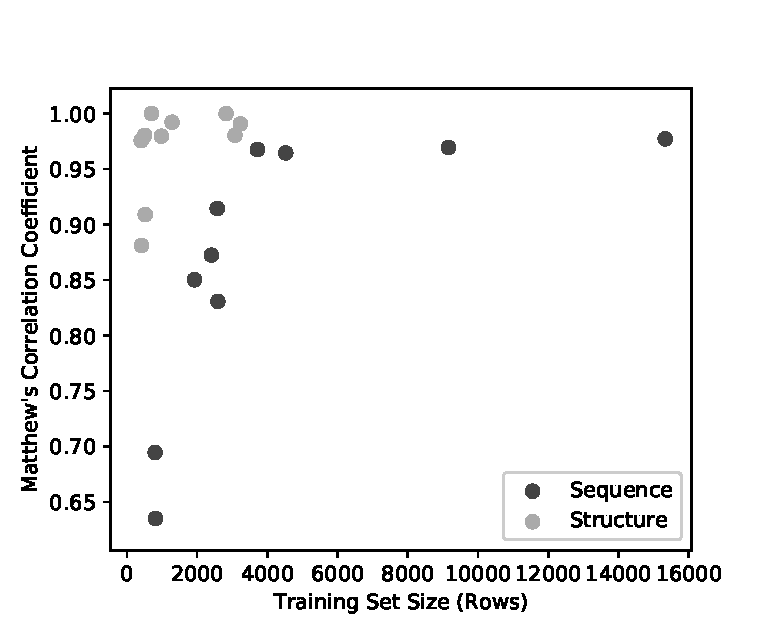
\includegraphics[width=1.0\textwidth]{Figures/size-score.eps}
\caption{\label{fig:size-score} Model Performance (MCC) as a function
  of training set size. Below ~4,000 rows, performance declines
  sharply, though above this threshold there ceases to be a strong
  correlation between the two.}
\end{figure}


\begin{figure}
\centering
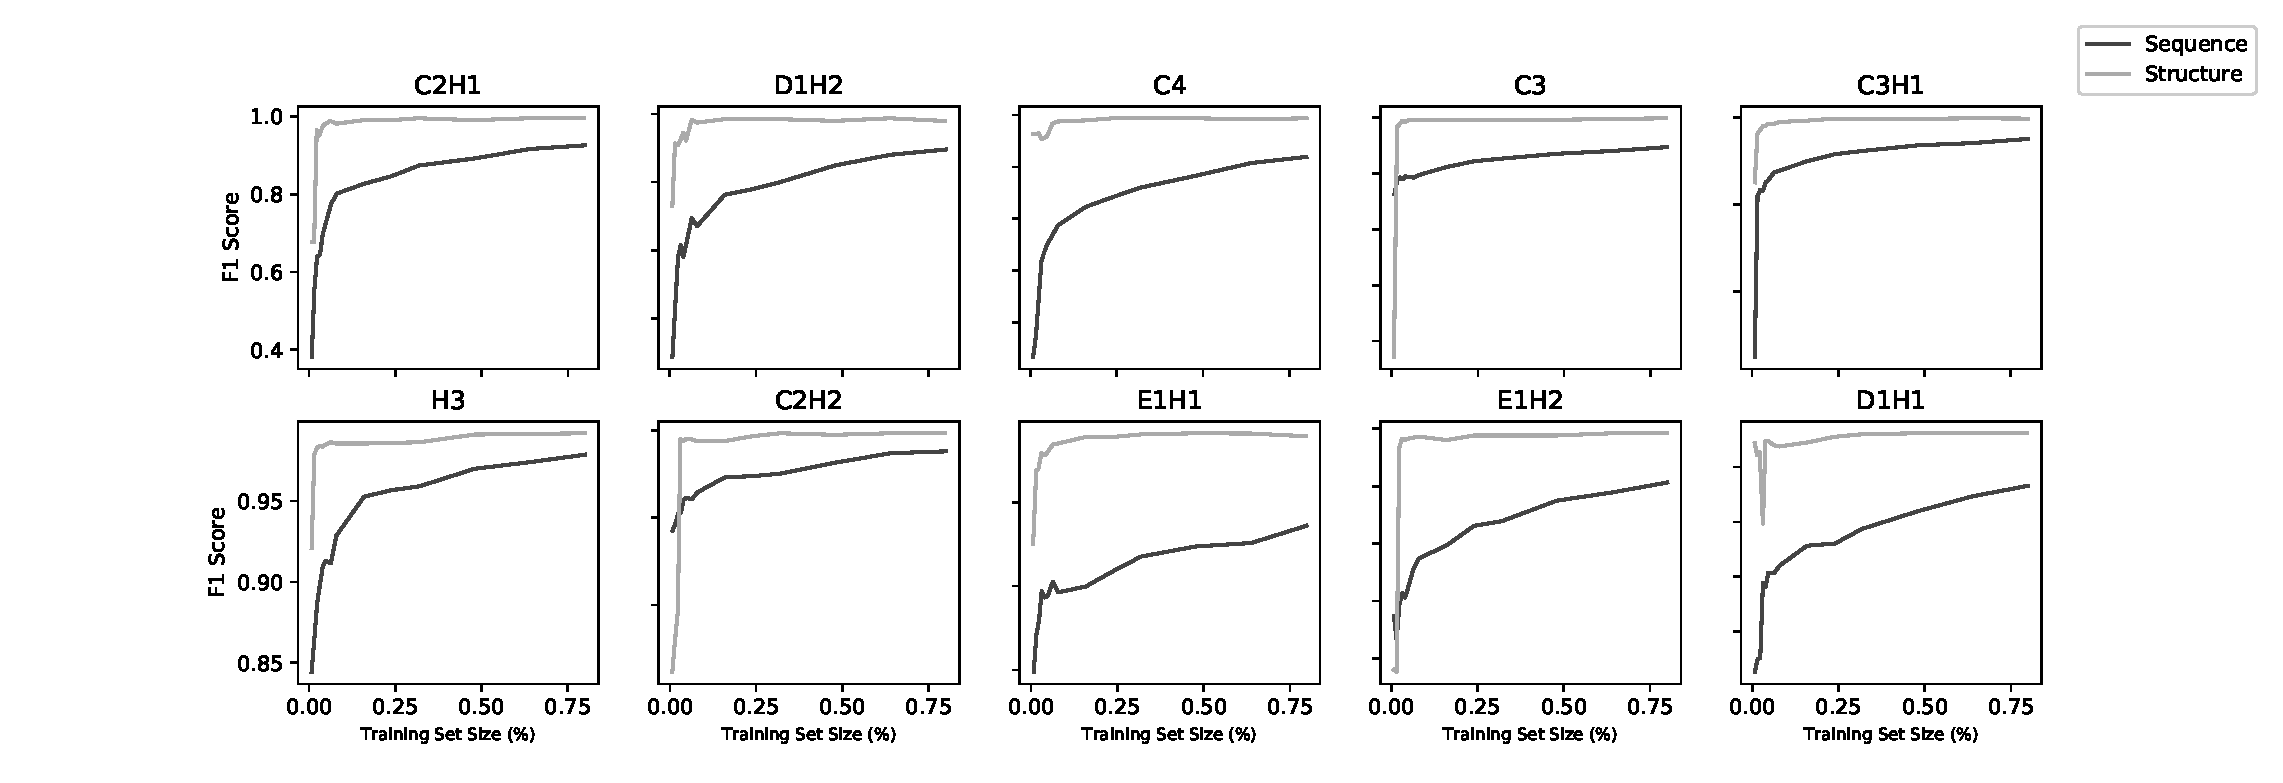
\includegraphics[width=1.0\textwidth]{Figures/learning-curve.eps}
\caption{\label{fig:learning-curves} Learning curves for all 20
  models. Each model was trained on increasing subsets of the overall
  training set using five-fold cross-validation. Sequence models
  improved with increasing dataset size, suggesting smaller dataset
  sizes would not be feasible, whereas structure models did not.}
\end{figure}

While the training is affected by dataset size, this does not appear to be a significant limiting factor for most of the models here. Figure~\ref{fig:size-score} shows the model performance (as MCC) for the sequence and structure models. The performance of the sequence models falls off as the dataset falls below a threshold number of data points in the low thousands --- as does the performance of the structural models. The lowest three performing structural models were also the lowest three in dataset size (C3, E1H1, D1H1), but two of these have only two residues so, as discussed above, the performance might not be expected to be very good.

Learning curves (Figure~\ref{fig:learning-curves}) using fractions of the datasets show a correlation with dataset size for the sequence models, but above around 1000 sequences, the structure models do not improve with larger datasets.

The level of abstraction used to describe both sequences and structures made it unlikely that any homology between data in the training and testing sets would artificially improve the performance. The features are largely calculated from residues around the binding residues, rather than the sequence in which they occur. However given the presence of similar sequences in the dataset, I thought it prudent to confirm that these were not artificially increasing the models' performance.

To this end, I wanted to explore what would happen if only unique sequences were used, whereby the available sequences are clustered on some similarity threshold, and one representative from each used. Different sequence identity thresholds were used for clustering with CD-HIT and a training set was created from this new set of sequences for each threshold, and used to create a model. When clustering at 40\% sequence identity (the lowest used), there was slightly lower performance but clustering at this level did result in smaller datasets. As indicated previously, this is a major determinant of these sequence models' performance, so I wanted to determine if this lowered performance was because the dataset size was smaller (which would mean the original models trained on all the data were not compromised) or if a model trained on unique sequences performed less well, which would call into question the high scores of my models as being due to such sequences.

\begin{figure}
\centering
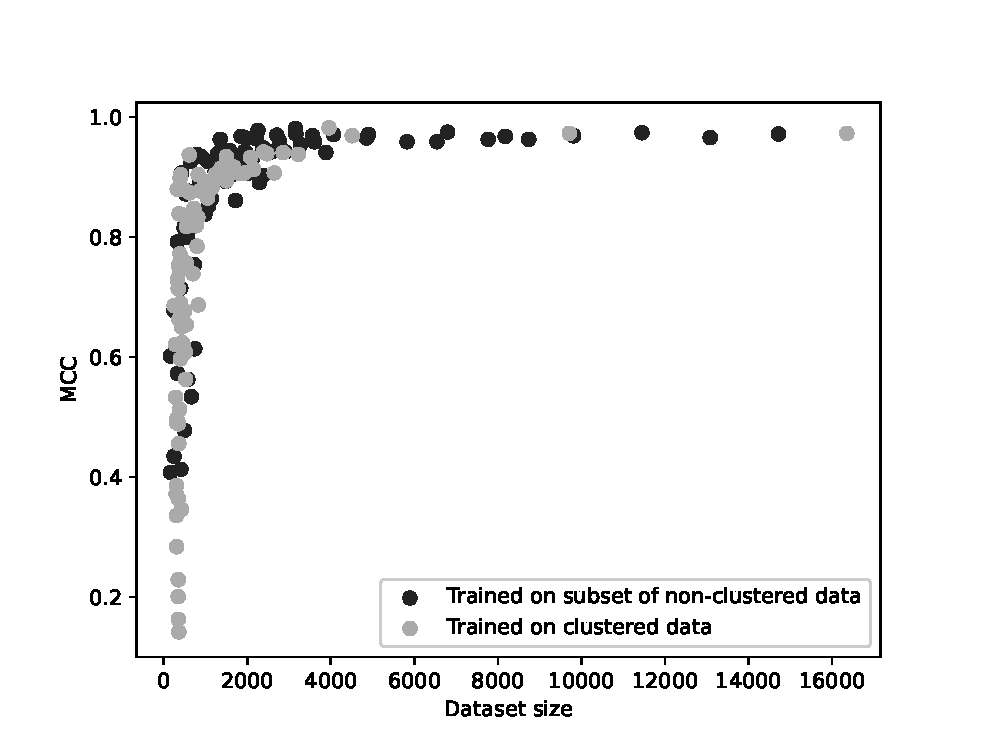
\includegraphics[width=1.0\textwidth]{Figures/clustering.eps}
\caption{\label{fig:clustering} MCC as a function of dataset size for
  160 different models.
  For each of the ten zinc-binding families, we trained a
  classifier on 20\%, 30\%, 40\%, 50\%, 60\%, 70\%, 80\%, 90\% and
  100\% of the original, unclustered data, and also a classifier
  trained on data with sequences clustered by 40\%, 50\%, 60\%, 70\%,
  80\%, 90\% and no clustering. Each of these models is shown here,
  with their performance (MCC) and size of the dataset used to train
  them. The two modes of dataset reduction are shown by different
  shades and it can be seen that the curves are not significantly
  different. A
  model's performance is a function of its dataset size, regardless of
  whether any removal of similar sequences is performed.}
\end{figure}

In order to identify whether this lowered performance was because the models performed worse without the possibility of homologous sequences between the training and test sets, or whether it was a result of the smaller training set,
for each zinc-binding family I trained a classifier on 20\%, 30\%, 40\%, 50\%, 60\%, 70\%, 80\%, 90\% and 100\% of the
original, unclustered data, and also a classifier trained on data with sequences clustered by 40\%, 50\%, 60\%, 70\%, 80\%, 90\% and with no clustering. The performance of the models was then plotted against the resulting dataset sizes as shown in Figure~\ref{fig:clustering}.  This demonstrates that it is dataset size that determines model performance, regardless of the similarity of the sequences in the training and testing datasets. For a given dataset, you could predict how well the model trained on it would perform based on dataset size alone --- the similarity of the sequences within that dataset made no difference when dataset size was held constant.

\begin{table}
  \caption{\label{tab:psiblast}Predictive ability of using BLAST alone
    to predict zinc binding in protein sequences using homology
    alone.}
\begin{center}
\begin{tabular}{llllll} \hline
Family & Dataset Size & Recall & Precision & F1    &  MCC  \\ \hline
C2H2   & 3960         & 0.99   & 0.95      & 0.97  &  0.94 \\
C3H1   & 9710         & 0.29   & 0.87      & 0.44  &  0.33 \\
C2H1   & 2154         & 0.24   & 0.88      & 0.37  &  0.3  \\
D1H1   & 818          & 0.05   & 0.8       & 0.09  &  0.11 \\
C3     & 2868         & 0.13   & 0.61      & 0.21  &  0.07 \\ 
E1H1   & 828          & 0.06   & 0.62      & 0.11  &  0.06 \\
D1H2   & 2470         & 0.03   & 0.53      & 0.06  &  0.01 \\
H3     & 5058         & 0.01   & 0.19      & 0.02  & -0.1  \\
E1H2   & 2648         & 0.02   & 0.33      & 0.04  & -0.06 \\ \hline
\end{tabular}
\end{center}
\end{table}

As an additional means of showing how little effect sequence similarity has on ability to predict zinc binding, I compared the sequence models with using BLAST for predicting zinc-binding sites. For each zinc-binding family, a BLAST database was created using 80\% of the available zinc-binding sequences, and BLAST's ability
to identify zinc binding sites from the remaining 20\% was compared against an equivalently sized negative set. Results are shown in Table~\ref{tab:psiblast}. With the exception of C2H2, using BLAST to find zinc binding based on homology performs much worse than the models presented here. Even in the case of C2H2, which seems to have much more similar sequences in its dataset, my model still narrowly outperforms BLAST.

However the models presented here are not intended to be general purpose zinc binding predictors that detect common properties of all zinc binding sites --- they are family-specific predictors based on the principle that common, specific types of zinc binding site have more identifiable, consistent properties than do zinc binding sites in general. As a result, they will not readily detect binding sites of uncommon zinc-binding families. This abstract predictiveness has been deliberately discarded to create highly effective models for specific, common families of zinc binding sites. It is also noteworthy that the binding site itself is a useful unit of prediction using this
methodology --- even for sequences --- rather than individual binding sites. The models are therefore identifying something biologically real (a zinc binding site) rather than something which does not actually exist in isolation (a single zinc binding residue), but which is a useful heuristic in some circumstances.

\begin{table}
  \caption{\label{tab:genome}Percentage of genome predicted to be zinc
    binding by ZincBindPredict for an assortment of bacterial
    genomes. Genomes were acquired from ensembl
    \cite{yates2020ensembl} in the form of translated polypeptide
    sequences, with a sequence labelled as zinc binding if any of the
    ten models finds at least one zinc binding site for that
    sequence/family combination. See Supplementary file {\tt
      genomes.zip} for the full results.}
\begin{center}
\begin{tabular}{ll} \hline
Species                          & Percentage of Genome   \\
                                 & Predicted Zinc Binding \\ \hline
{\it Campylobacter jejuni}       & 6.4\%                  \\
{\it Clostridioides difficile}   & 5.8\%                  \\
{\it Enterococcus faecalis}      & 7.5\%                  \\
{\it Listeria monocytogenes}     & 7.9\%                  \\
{\it Mycobacterium tuberculosis} & 11.3\%                 \\
{\it Salmonella enterica}        & 11.1\%                 \\
{\it Shigella flexneri}          & 10.1\%                 \\ 
{\it Streptococcus pneumoniae}   & 7.6\%                  \\ \hline

\end{tabular}
\end{center}
\end{table}

A demonstration of this can be seen by applying the sequence models to bacterial genomes to measure the proportion of typical genomes that the models predict to be zinc binding, as shown for a range of bacterial genomes in Table~\ref{tab:genome}. For most genomes, fewer than 10\% of proteins are flagged as zinc binding, with the average for the genomes examined being 8.46\%. Given that the zinc-binding families for which predictors have been generated represent 67.0\% of binding sites in ZincBindDB, this would imply a `true' predicted proportion of 12.6\% which is a little higher than the widely cited figure of 10\%.

\section{Access to Models}

The models are available through a web app called ZincBindPredict. This is a GraphQL API, like the ZincBindDB database API, which allows users to submit jobs and get the results. A GraphQL request can be sent with either a protein sequence or protein structure, and a job ID will be returned (see Figure~\ref{fig:zbp-mutation}). This can then be polled for results as the protein or sequence is searched using each model in turn, with the identified binding sites returned as a list with the associated probability (see Figure~\ref{fig:zbp-query}). Internally, when a protein is submitted a `job' folder is created, using the current UNIX time in milliseconds as the ID. This job ID is returned to the user, which they can use to query the status of the job, as a script which runs each of the model in turn runs as a background process and saves its results to the job's folder on the server, for inspection by the API.

The ZincBind web interface that was explored in-depth in Chapter 3 also has a page that allows users to submit jobs using a more human-friendly interface, which itself consumes the ZincBindPredict API (see Figure~\ref{fig:prediction-interface}). The user is prompted to provide the representation of a protein - either as a structure file, a sequence file, or a FASTA sequence pasted in. They also have the option of only searching for specific families. Positive results are listed on a results page once the job is complete, and the number of rejected residue combinations is listed.

\begin{figure}
\centering
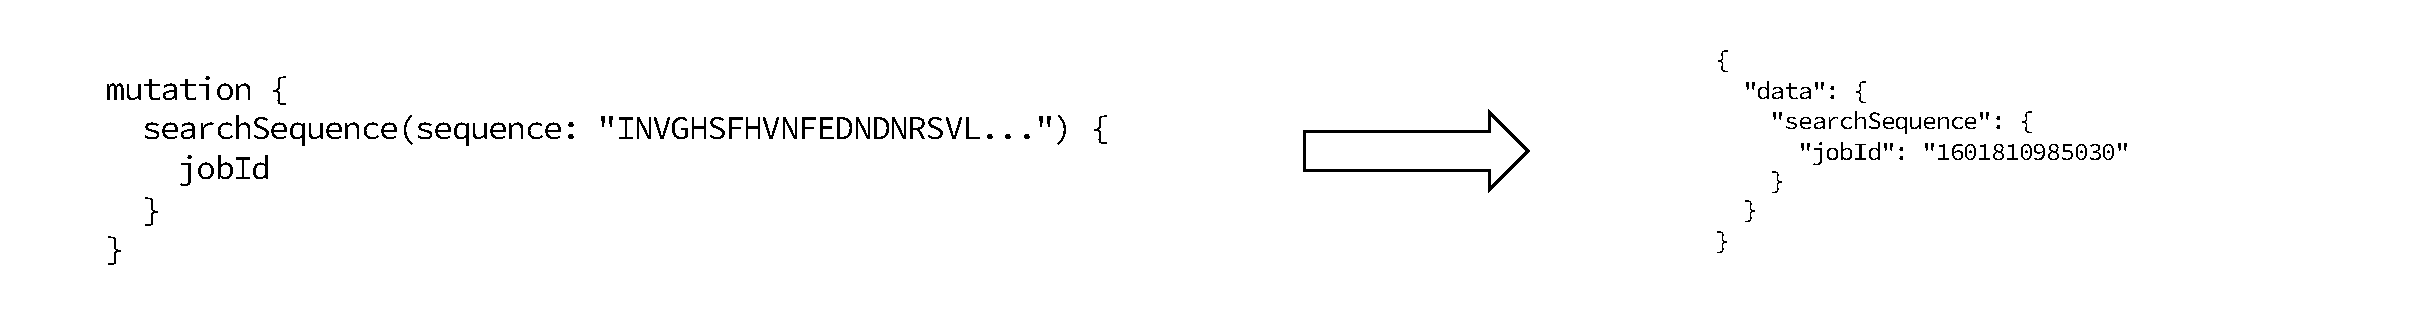
\includegraphics[width=1.0\textwidth]{Figures/zbp-mutation.eps}
\caption{\label{fig:zbp-mutation} A mutation from the ZincBindPredict API. Mutations
begin with the mutation identifier to indicate that the top level \texttt{Mutation} object
is what the \texttt{searchSequence} mutation belongs to --- queries can begin with
\texttt{query} too but this is optional. Here the sequence is being given as an
argument, and the ID of the job is returned.}
\end{figure}

\begin{figure}
\centering
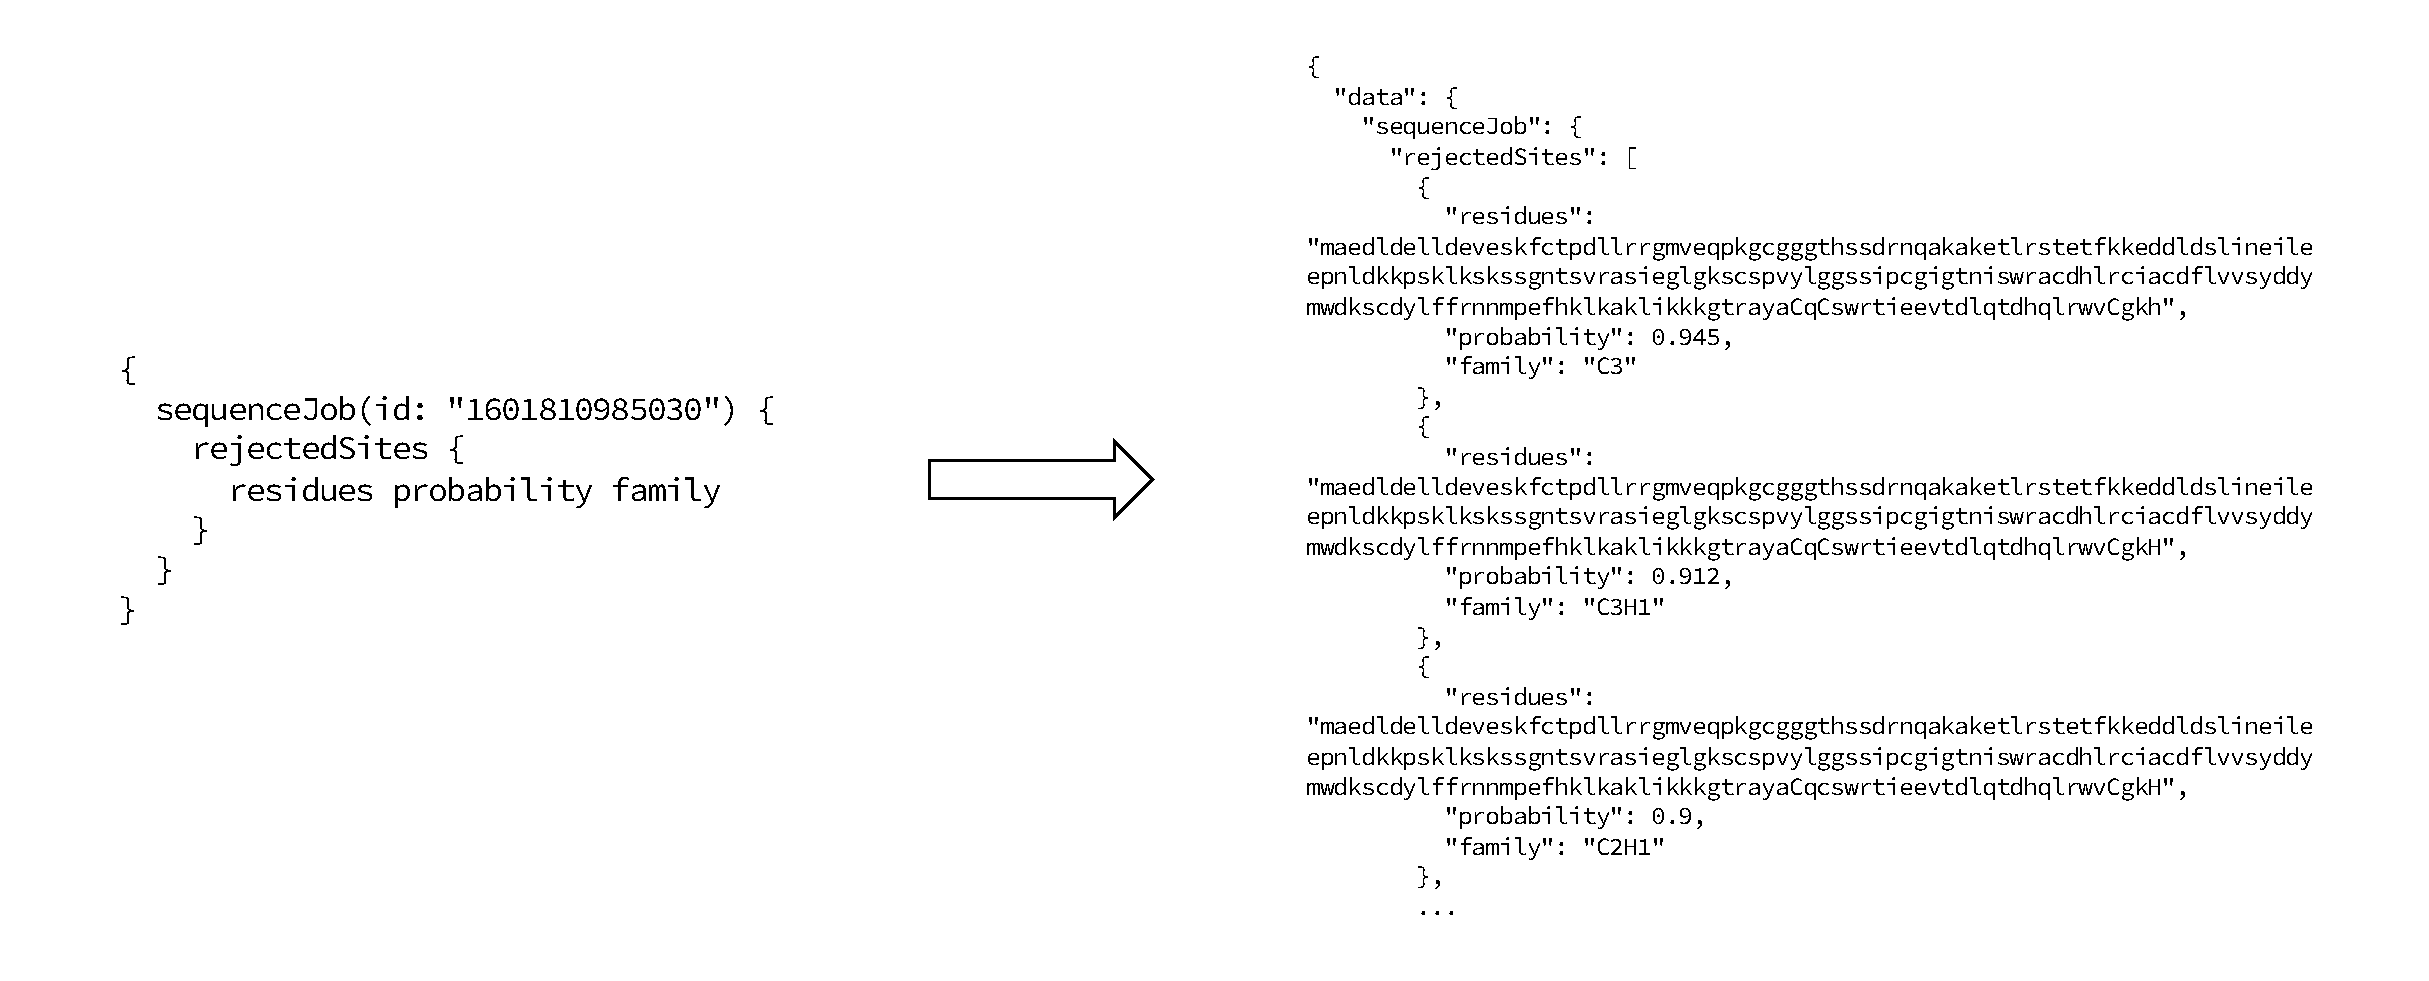
\includegraphics[width=1.0\textwidth]{Figures/zbp-query.eps}
\caption{\label{fig:zbp-query} A query for the results of a ZincBindPredict job.
The ID of the job is supplied, and this particular query requests the status of
the job, as well the predicted sites. The rejected sites can also be requested,
but since they are quite numerous, typically the flexibility of GraphQL in allowing
you to choose to omit them is useful in conserving network resources.}
\end{figure}

\begin{figure}
\centering
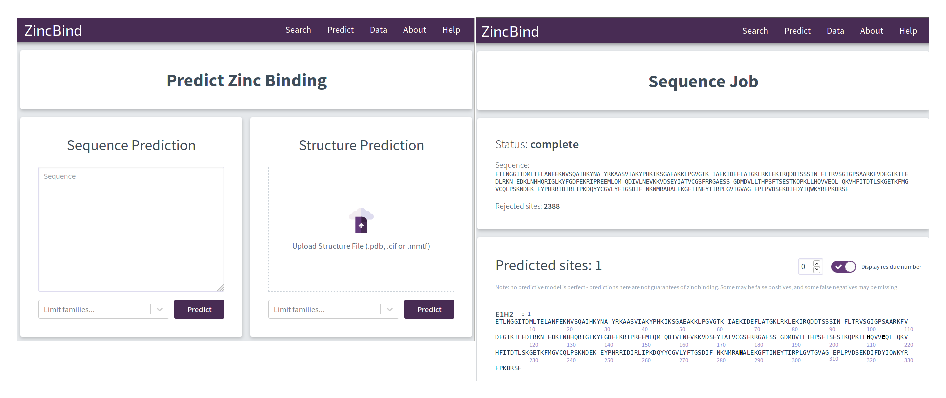
\includegraphics[width=1.0\textwidth]{Figures/prediction-interface.eps}
\caption{\label{fig:prediction-interface} The prediction page on the ZincBind web interface, and an example of a predicted zinc binding site in a protein sequence.}
\end{figure}

\section{Conclusion}

The models created here are highly effective, albeit at a very particular task. They are not predictors of zinc binding in general, and they will not generally detect zinc binding sites of obscure families and residue combinations. They were never intended to. A deliberate trade-off between model effectiveness and model generalisability has been made in order to demonstrate the principal that properties of binding sites within families \emph{are} more tightly distributed and hence create more accurate models. These models also detect something biologically real --- full binding sites --- rather than individual zinc binding residues which, as discussed, are an artificial concept.

However, this downside is not necessarily permanent. The models are limited to these ten models because these are the families for which there is sufficient (only just, in the case of some of the sequence models) data to train a classifier. However, the data in ZincBind is constantly growing thanks to the automated database update scripts in place. Over the time, the eleventh-placed model will acquire enough data to warrant a model, and then the twelfth, and so on. The dataset-size threshold for training is not relative to the total size of the database, it is an absolute amount, and so over time more and more families will be able to have models trained for them, and the models will become more comprehensive of zinc binding generally. The benefits of this trade-off are permanent --- the deficiencies are temporary.







%%%% MACRO DEFINITION %%%%

\providecommand{\pvivax}{P.~vivax}
\providecommand{\pfalciparum}{P.~falciparum}
\providecommand{\cterm}{C-terminus}
\providecommand{\nterm}{N-terminus}

\providecommand{\e}[1]{\ensuremath{\times 10^{#1}}}
\newcolumntype{P}[1]{>{\centering\arraybackslash}p{#1}}
\newcolumntype{M}[1]{>{\centering\arraybackslash}m{#1}}

\providecommand{\refimage}[1]{\figurename~\ref{fig:#1}}

%TC:macro \note [ignore]



%%%%%%%%%%%%%%%%%%%%%%%%%%%%%%%%%%%%%%%%%%%%%%%%%%%%%%%%%%%%%%%%%%%%%%%%%%%%%%%%%%%%%%%%%%%%%%%%%%%%%%%%%%%%%%%%%%%%%
%%%%%%%%%%%%%%%%%%%%%%%%%%%%%%%%%%%%%%%%%%%%%%%%%%%%%%%%%%%%%%%%%%%%%%%%%%%%%%%%%%%%%%%%%%%%%%%%%%%%%%%%%%%%%%%%%%%%%
%													BEGIN
%%%%%%%%%%%%%%%%%%%%%%%%%%%%%%%%%%%%%%%%%%%%%%%%%%%%%%%%%%%%%%%%%%%%%%%%%%%%%%%%%%%%%%%%%%%%%%%%%%%%%%%%%%%%%%%%%%%%%
%%%%%%%%%%%%%%%%%%%%%%%%%%%%%%%%%%%%%%%%%%%%%%%%%%%%%%%%%%%%%%%%%%%%%%%%%%%%%%%%%%%%%%%%%%%%%%%%%%%%%%%%%%%%%%%%%%%%%

\chapter{Predicting Zinc Binding Sites} % Write in your own chapter title
\label{Chapter5}
\lhead{Chapter 5. \emph{Predicting Zinc Binding in Proteins}} % Write in your own chapter title to set the page header

\emph{Note that some of the material in this chapter has been published in the journal Molecules under the title `Zincbindpredict—Prediction of Zinc Binding Sites in Proteins' (2021).}

The aim of this part of the PhD is to create a system which conceptually is quite simple --- it would take as its input a protein sequence or protein structure, and output a list of zero or more residue combinations which are predicted to form a zinc binding site, with an accompanying probability.

This system is a machine learning system; it uses binary classifiers trained on the large dataset of zinc binding sites described in the previous chapter which `learn' what zinc binding sites look like from that data.

This chapter will describe the approach taken to solving this problem, the models created, the architecture of the system from the user's point of view, and how the models are accessed and used.

\section{Approach}

As explored in Chapter 2, there have been multiple studies in the past which have used machine learning (or simpler methods) to create zinc-binding predictors (or general-purpose metal-binding predictors). Many of the general principles of these studies are adopted here, however there are two crucial methodological changes that have been made.

One recurring feature of previous work, particularly in the sequence-based predictive models, is the focus on zinc binding \emph{residues} rather than zinc binding \emph{sites}. In most cases, the entity examined by the predictive model is the individual residue, often with a surrounding linear sequence `window' of residues. The model then assigns a probability as to whether that residue is a zinc binding residue. As outlined in that chapter, this approach has had a measure of success, but it is a somewhat artificial concept. There is, after all, no such thing as a zinc-binding residue in isolation. The individual residues of a high-affinity zinc binding site of the kind considered here are only zinc-binding when the other residues are present, and conversely many non-zinc-binding residues could bind zinc if other residues were present in the correct locations. It is particular \emph{combinations} of residues, not individual residues, which are zinc binding --- an important fact not usually considered in research of this kind. As this chapter will explain, models have been created here which inspect residue combinations, not single residues.

Another commonality is the treatment of zinc binding sites as a single category, and the presumption of properties that are common to them all regardless of the residues of which they are comprised. This may well be sufficient, particularly as there are essentially only four residues that make up the vast majority of zinc binding sites, but it is possible that properties used for prediction have much tighter distributions within particular sub-categories of zinc binding sites. As such, rather than creating a single model that predicts zinc binding in structures and another that predicts them in sequence, one model has been created per \emph{family} of zinc binding site, of the kind described in Chapter 4 \footnote{`Family' is used in the sense of the family of liganding residues and is not related to homologous families.}. That is, there is a model for predicting H3 binding sites (those made of three histidine residues) in structure, one for predicting H3 binding sites in sequence, one for predicting C2H2 binding sites in structure, one for predicting C2H2 sites in sequence, and so on. As well as the increased specificity this affords, another advnatage of this approach is a purely practical one. All the possible H3 binding sites in a protein are found by taking all combinations of three histidine residues, and while the combinatorics of this can lead to large numbers of potential sites to check, it is vastly smaller than the combinations of \emph{all} residues that would need to be checked if the model were supposed to look for generic zinc binding sites --- an infeasible task for all but the smallest of proteins as the number of residue combinations quickly becomes impractically enormous.

The overall pipeline of the resulting system for predicting zinc binding then, is that when a protein structure or sequence is given, for each family for which there is a model, all residue combinations within that protein which match the family are identified (all unique combinations of three histidine residues for H3, for example) and passed to the relevant model, which assigns a probability that the residues comprise a zinc binding site, as well as making a binary yes-or-no prediction. This is repeated for every combination, and for every family, to build up a list of predicted binding sites.

\section{Data Preparation}

The first decision to make was which families to use. There are 701 families in total in ZincBind, ranging from C4 with its 3069 unique representatives, to obscure families like C1D1E1H2 (one cysteine, one glutamate, one aspartate and two histidine residues) which has only one representative. In fact there are 244 families with one representative, and many with only a small number of representatives. To train a model that can recognise some combination of residues as being a zinc binding site of some family rather than some random combination, the model needs to be trained on many examples of such sites, so there is clearly a minimum number of representatives in the database that a family must have for it to make sense to train a model for it. It is not immediately obvious what this minimum number should be. Initially it was decided to use the top ten families: C4, C3H1, C2H2, D1H2, E1H2, H3, C3, E1H1, C2H1 and D1H1. This was originally a somewhat arbitrary cutoff and the intention was to adjust it based on results, though as this chapter will show, ten families is probably the correct number in terms of resultant dataset size.

For a binary classifier of the kind being created here, the training set is a collection of positive samples (combinations of residues of that family which represent zinc binding sites) and negative samples (combinations of residues of that family which are not zinc binding sites). An assumption being made here is that if a combination of residues does not have a zinc atom bound to it in a structure, it is not a zinc binding site. This may not be true occasionally, as the structure simply may not have been crystallised in the presence of zinc. For this reason, some of the negative samples in the training sets may actually be positive. It is assumed however, that these cases are sufficiently infrequent as to have a negligible effect.

The residue combinations are represented in the training data as a vector of measurements, with the final measurement being the indicator of whether it is positive (1) or negative (0). Each row in the training data represents a residue combination, each column a feature. There are twenty training datasets altogether; for each of the ten families there is a training set for sequence data and a training set for structural data.

\subsection{Sequence Training Data}

To generate the sequence training datasets, for each family the ZincBind API was queried for all binding sites of that family, and those split over multiple chains were removed to leave single sequence binding sites --- the multi-chain zinc binding sites do not have a single sequence containing all the necessary residues in the combination. The resulting sequences were turned into feature vectors which contained the number of residues between each pair of binding residues, the average hydrophobicity (Wimley and White’s scale \cite{wimley:hphob}) of residues either side of the binding residues, using windows of size 1, 3 and 7, and the average number of charged residues either side of the binding residues, using the same window sizes. These fetaures are summarised in Table~\ref{tab:features}. This created a dataset of positive samples.

For the negative samples, for each family a sequence was chosen at random from the set of all unique sequences in UniProtKB and a combination of residues within that sequence matching the family but not a known binding site, was selected --- this was done repeatedly until a list of negative samples was built up equal in size to the
positive dataset.  The two datasets were combined into a single dataset for each family. The resultant dataset is summarised in Table~\ref{tab:dataset-size}.

\subsection{Structure Training Data}

To generate the structure training datasets, for each zinc-binding family, all relevant zinc binding sites belonging to a PDB structure with resolution better than 2~{\AA} were downloaded. As many of the measurements made are geometric, precise atom distances are important, and structures with too poor a resolution would create unreliable data for this purpose. For each PDB entry, the structure was downloaded and parsed using the Python library atomium (see Chapter 4), assembled into the correct biological assembly, and then each binding site was turned into a feature vector using the following measurements: mean inter C$\alpha$ distance of the liganding residues, standard deviation of the C$\alpha$ distances, minimum C$\alpha$ distance, maximum C$\alpha$ distance --- and the corresponding measurements for the C$\beta$ atoms, for a total of 8 geometric features. The distances used are all the pairwise combinations of the atoms involved, so H3 sites will have three inter C$\alpha$ distances, C4 sites will have six, and so on. The final feature is the `hydrophobicity contrast function', calculated at the centre of the C$\beta$ atoms with a radius of 7~{\AA}, This algorithm is a measure of how much outer atoms in a sphere are more hydrophobic than inner atoms, with higher values previously shown to be associated
with centres of metal binding \cite{yamashita1990metal,gregory1993prediction}, as described in Chapter 1.

As with the sequence data, this was repeated on combinations of residues with no known zinc binding ability until there was an equal number of negative samples. For these, PDB structures with no zinc atoms were selected at random (random sampling with replacement), and any random combination of residues from within that structure which matched the binding site family in question was selected. The resultant dataset is summarised in Table~\ref{tab:dataset-size}.

\begin{table}
  \caption[Training set size.]{\label{tab:dataset-size}The sizes of the twenty training set sizes used to train the models. In each case the size is less than the theoretical maximum of double the total number of sites per family, because the sequence sites have those with multiple chains filtered out, and the structure sites have those from poor resolution structures filtered out.}
\begin{center}
\begin{tabular}{lll} \hline
Family & Structure Dataset Size & Sequence Dataset Size \\ \hline
C4     & 2825         &  15332  \\
C3H1   & 3232         &  9158   \\
H3     & 3078         &  4524   \\
E1H2   & 1287         &  2574   \\
C2H2   &  702         &  3715   \\
D1H2   &  982         &  2406   \\
C3     &  407         &  2591   \\
C2H1   &  506         &  1926   \\
D1H1   &  522         &  804    \\ 
E1H1   &  416         &  812    \\ \hline
\end{tabular}
\end{center}
\end{table}

\begin{table}
  \caption[Feature generation.]{\label{tab:features}Details of how features are calculated
    for residue combinations in structure and sequence models.
    Hydrophobicity of sequence residues is defined using Wimley and
    White's scale \protect\cite{wimley:hphob}, charge is the count of
    charged residues (aspartate, glutamate, arginine, histidine and
    lysine).}
\begin{center}
\begin{tabular}{ll} \hline
Model type            &  Feature                                              \\ \hline
{\bfseries Sequence}  &                                                       \\
                      &  Inter-residue distance (one per gap)                 \\
                      &  Average hydrophobicity around residues (window 1)    \\            
                      &  Average hydrophobicity around residues (window 3)    \\
                      &  Average hydrophobicity around residues (window 5)    \\
                      &  Average number of charges around residues (window 1) \\
                      &  Average number of charges around residues (window 3) \\
                      &  Average number of charges around residues (window 5) \\
{\bfseries Structure} &                                                       \\
                      &  Mean Inter-C$\alpha$ distance                        \\
                      &  Maximum Inter-C$\alpha$ distance                     \\
                      &  Minimum Inter-C$\alpha$ distance                     \\
                      &  Inter-C$\alpha$ distance standard deviation          \\
                      &  Mean Inter-C$\beta$ distance                         \\
                      &  Maximum Inter-C$\beta$ distance                      \\
                      &  Minimum Inter-C$\beta$ distance                      \\
                      &  Inter-C$\beta$ distance standard deviation           \\
                      &  Hydrophobic contrast (radius 4~{\AA})                \\ \hline
\end{tabular}
\end{center}
\end{table}

\section{Model Training}

While the quality and size of the training set is a large determinate of eventual model quality, the choice of machine learning algorithm is also crucial. Chapter 2 explored the history of metal binding site predictive models and the various algorithms used --- as expanded upon there, there has been a shift towards the use of artificial neural networks over the past five years. The primary reason behind this shift has been the vast increase in the size of available datasets, which are generally required for something which uses as many layers of abstraction as neural networks. As the datasets here are necessarily quite small compared with those datasets (a deliberate tradeoff made in the hopes of creating highly specific models), it was decided that such algorithms were not appropriate.

K-Nearest Neighbor, Support Vector Machines, and Random Forest algorithms were therefore considered. Originally, the intention was to train a model with each of these algorithms and have the final model be a consensus of these three whereby they vote on each incoming residue combination. However early testing showed that Random Forest so consistently and significantly outperformed both the other two models in isolation, and the resultant consensus model, that it was ultimately decided to solely use Random Forest for training.

The actual training of the models was done using the Python library scikit-learn \cite{scikit-learn}. For each training dataset, the data was randomly split into training and test data using an 80:20 split --- the former used to train, the latter used to evaluate. As explained in Chapter 2 this is vital to ensure the resultant model is not overfit.

The hyper-parameters for each model were selected separately using 5-fold cross validation of the training set. The hyper-parameters explored were the impurity measure (gini vs.\ entropy --- the algorithm used to split individual trees at each node), the maximum depth that the component trees could have (4, 6, 8 or no maximum), the number of trees in the forest (10, 100 or 1000), and the means of determining the best number of features at each split (either the
square root of the number of features, or the log$_2$ of the number of features). Once optimal hyper-parameters were identified (determined by which combination produced the best MCC score in the cross-validation), the models were trained with those hyper-parameters using the entire training dataset.

Once the model was trained on the ideal hyperparameters using all the training data, the model was evaluated on the test data, and the true positive, false positive, true negative and false negative counts were calculated. From these the recall, precision, F1 score, and Matthews' Correlation Coefficient were calculated. All of these were saved to the model by making them properties of the actual Python object, and then this Python object was serialised to disk using the Python `joblib' library for later use.

\section{Model Performance}

For the structural models, the lowest MCC score was 0.88 (for the E1H1 model). This, and the D1H1 model (MCC=0.91), relies on the geometry between just two residues, which makes creating a distinct separation between the two classes somewhat more difficult --- though their performance is still very close behind the three-residue and four-residue family models. The structure models had an average MCC of 0.960 (see Table~\ref{tab:structure}).

The sequence models also had high scores, though were more variable. The four-residue sites in particular had highly conserved patterns of residue spacing and flanking hydrophobicity despite being from several homologous families. The average MCC score for the sequence models was 0.87, with the lowest MCC being 0.61 for the E1H1 model and 0.74 for the D1H1 model --- again the two two-residue models were some way behind the MCC of 0.84 for the C3 model (see Table~\ref{tab:sequence}).

The high performance of the models appears to justify the methodological changes made compared with previous metal binding classifiers. The performance scores here compare favourably with recent comparable predictive models based on structure and sequence covered in Chapter 2 --- most notably the `SVM and Sample-weighted Probabilistic Neural Network' (MCC$=0.80$) \cite{li2019}, the `meta-zinc predictor' (MCC$=0.79$) \cite{li2017} and ZincExplorer (MCC$=0.78$) \cite{chen2013}.

\begin{table}
  \caption[Structural model performance.]{\label{tab:structure}Results for structure models, sorted
    by Matthews Correlation Coefficient (MCC). The two-residue
    families' performance was lower than the others as there is
    essentially just the measurements between two centres to perform
    the classification, but still scored relatively
    highly. Four-residue sites in particular were found to have very
    predictable properties.}
\begin{center}
\begin{tabular}{llllll} \hline
Family & Dataset Size & Recall & Precision & F1    & MCC  \\ \hline
C2H2   &  702         & 1.00   & 1.00      & 1.00  & 1.00 \\
C4     & 2825         & 1.00   & 1.00      & 1.00  & 1.00 \\
C3H1   & 3232         & 1.00   & 0.99      & 1.00  & 0.99 \\
E1H2   & 1287         & 1.00   & 0.99      & 1.00  & 0.99 \\
C2H1   &  506         & 1.00   & 0.98      & 0.99  & 0.98 \\
H3     & 3078         & 1.00   & 0.98      & 0.99  & 0.98 \\
D1H2   &  982         & 1.00   & 0.98      & 0.99  & 0.98 \\
C3     &  407         & 1.00   & 0.98      & 0.99  & 0.98 \\
D1H1   &  522         & 1.00   & 0.91      & 0.95  & 0.91 \\ 
E1H1   &  416         & 0.93   & 0.95      & 0.94  & 0.88 \\ \hline
\end{tabular}
\end{center}
\end{table}

\begin{table}
\caption[Sequence model performance]{\label{tab:sequence}Results for sequence models, sorted by
  Matthews Correlation Coefficient (MCC).}
\begin{center}
\begin{tabular}{llllll} \hline
Family & Dataset Size & Recall & Precision & F1    & MCC  \\ \hline
C4     & 15332        & 1.00   & 0.98      & 0.99  & 0.98 \\
H3     & 4524         & 0.98   & 0.99      & 0.98  & 0.97 \\
C2H2   & 3715         & 0.97   & 0.99      & 0.98  & 0.95 \\
C3H1   & 9158         & 0.98   & 0.96      & 0.97  & 0.94 \\
E1H2   & 2574         & 0.95   & 0.97      & 0.96  & 0.92 \\
D1H2   & 2406         & 0.94   & 0.95      & 0.94  & 0.90 \\
C2H1   & 1926         & 0.93   & 0.95      & 0.94  & 0.88 \\
C3     & 2591         & 0.95   & 0.89      & 0.92  & 0.84 \\
D1H1   & 804          & 0.80   & 0.93      & 0.86  & 0.74 \\
E1H1   & 812          & 0.81   & 0.83      & 0.82  & 0.61 \\ \hline
\end{tabular}
\end{center}
\end{table}

\begin{figure}
\centering
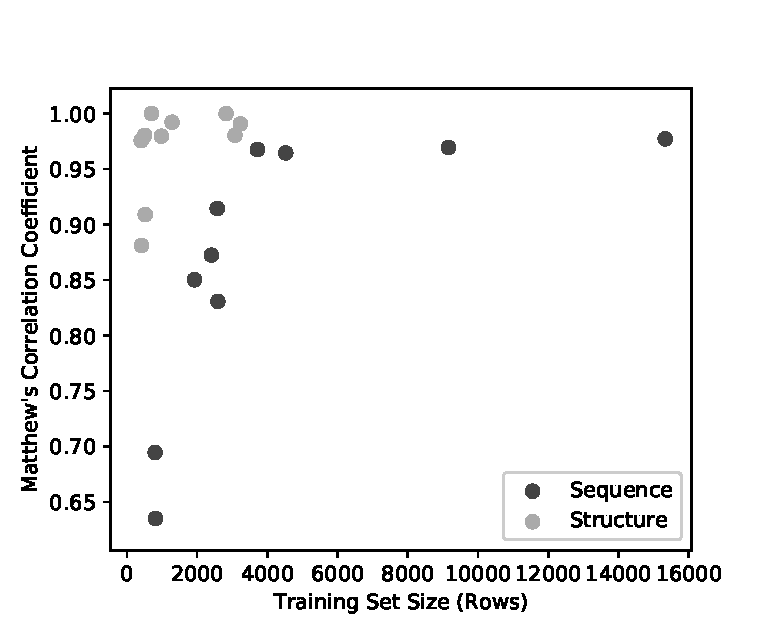
\includegraphics[width=1.0\textwidth]{Figures/size-score.eps}
\caption[Model Performance (MCC) as a function of training set size.]{\label{fig:size-score} Model Performance (MCC) as a function
  of training set size. Below ~4,000 rows, performance declines
  sharply, though above this threshold there ceases to be a strong
  correlation between the two.}
\end{figure}


\begin{figure}
\centering
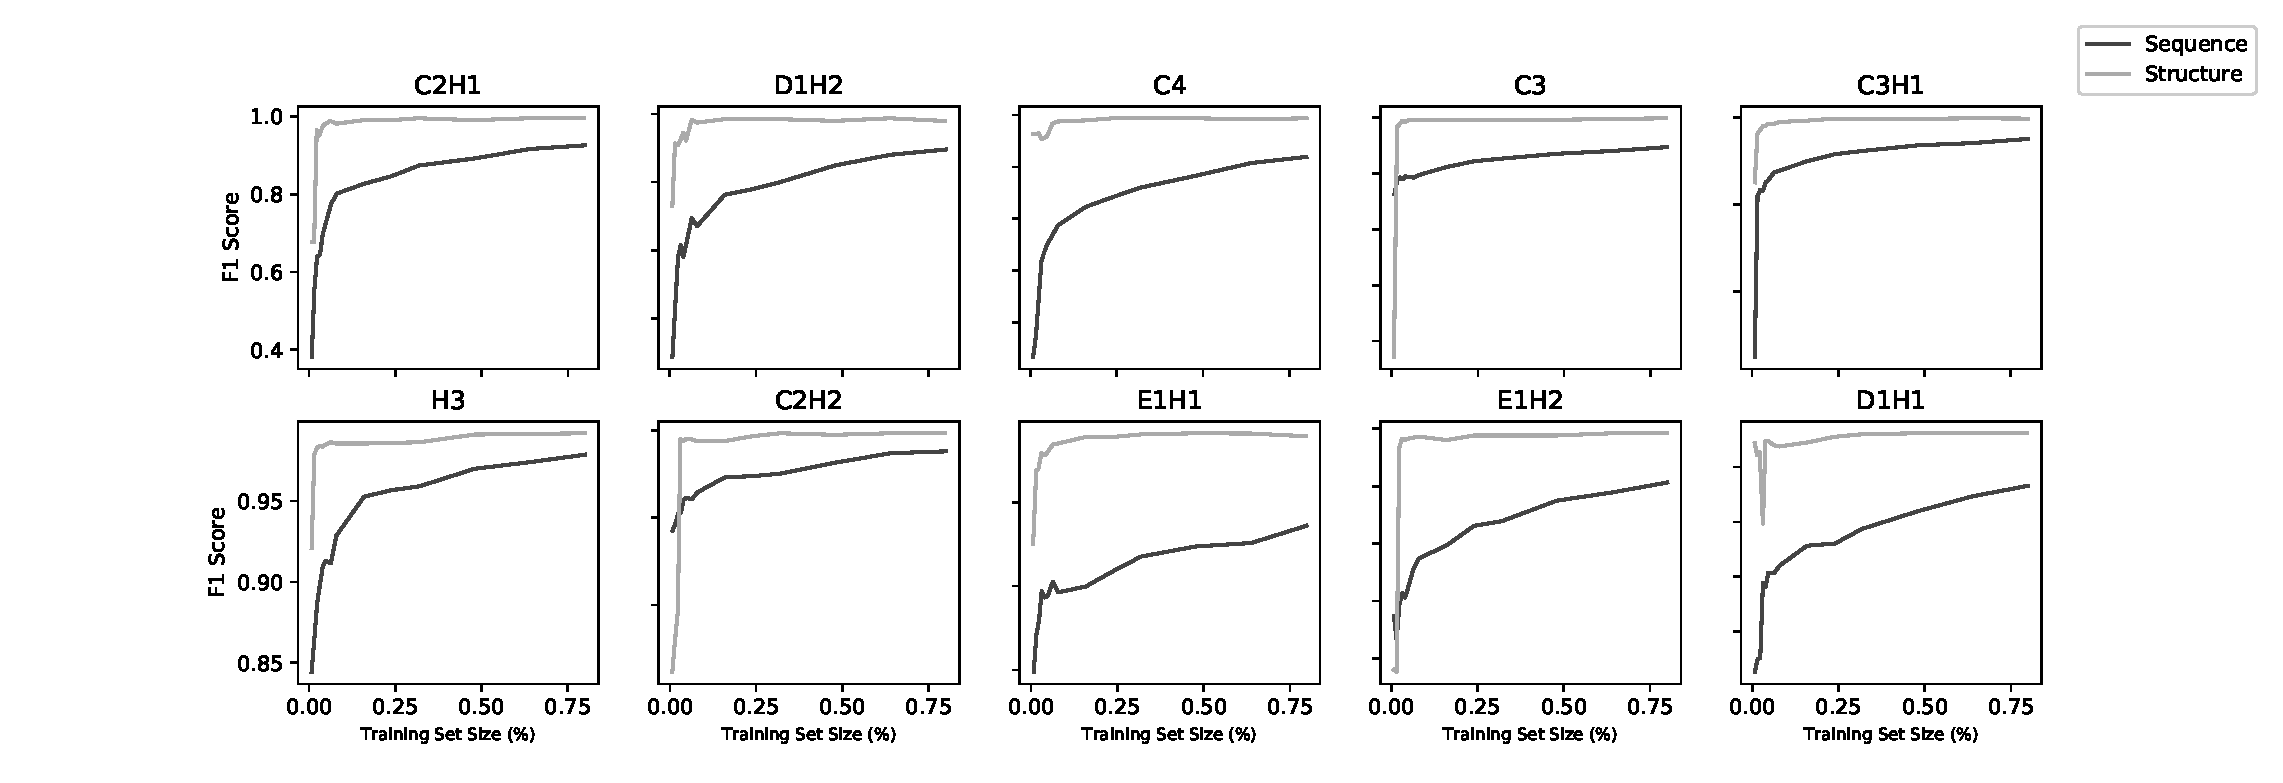
\includegraphics[width=1.0\textwidth]{Figures/learning-curve.eps}
\caption[Learning curves for all 20 models.]{\label{fig:learning-curves} Learning curves for all 20
  models. Each model was trained on increasing subsets of the overall
  training set using five-fold cross-validation. Sequence models
  improved with increasing dataset size, suggesting smaller dataset
  sizes would not be feasible, whereas structure models did not.}
\end{figure}

While the training is affected by dataset size, this does not appear to be a significant limiting factor for most of the models here. Figure~\ref{fig:size-score} shows the model performance (as MCC) for the sequence and structure models. The performance of the sequence models falls off as the dataset falls below a threshold number of data points in the low thousands --- as does the performance of the structural models. The lowest three performing structural models were also the lowest three in dataset size (C3, E1H1, D1H1), but two of these have only two residues so, as discussed above, the performance might not be expected to be very good.

Learning curves (Figure~\ref{fig:learning-curves}) using fractions of the datasets show a correlation with dataset size for the sequence models, but above around 1000 sequences, the structure models do not improve with larger datasets.

The level of abstraction used to describe both sequences and structures made it unlikely that any homology between data in the training and testing sets would artificially improve the performance. The features are largely calculated from residues around the binding residues, rather than the sequence in which they occur. However given the presence of similar sequences in the dataset, it was thought prudent to confirm that these were not artificially increasing the models' performance.

To this end, the aim was to explore what would happen if only unique sequences were used, whereby the available sequences are clustered on some similarity threshold, and one representative from each used. Different sequence identity thresholds were used for clustering with CD-HIT and a training set was created from this new set of sequences for each threshold, and used to create a model. When clustering at 40\% sequence identity (the lowest used), there was slightly lower performance, but clustering at this level did result in smaller datasets. As indicated previously, this is a major determinant of these sequence models' performance, so it was necessary to determine if this lowered performance was because the dataset size was smaller (which would mean the original models trained on all the data were not compromised) or if a model trained on unique sequences performed less well, which would call into question the high scores of the models as being due to such sequences.

\begin{figure}
\centering
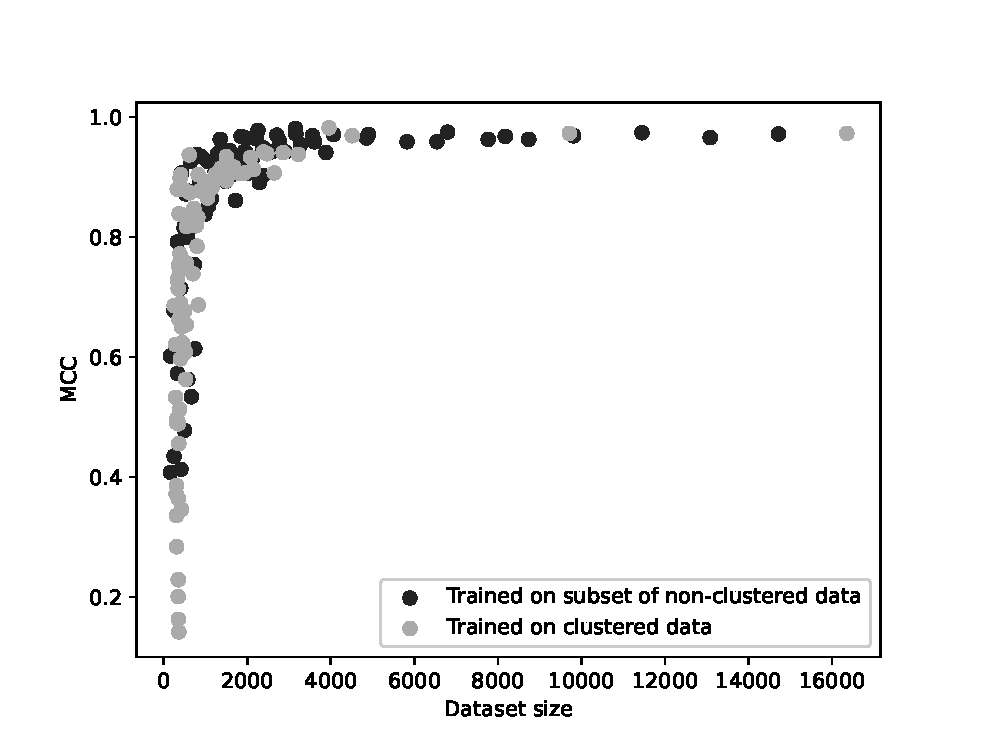
\includegraphics[width=1.0\textwidth]{Figures/clustering.eps}
\caption[MCC as a function of dataset size for 160 different models.]{\label{fig:clustering} MCC as a function of dataset size for
  160 different models.
  For each of the ten zinc-binding families, we trained a
  classifier on 20\%, 30\%, 40\%, 50\%, 60\%, 70\%, 80\%, 90\% and
  100\% of the original, unclustered data, and also a classifier
  trained on data with sequences clustered by 40\%, 50\%, 60\%, 70\%,
  80\%, 90\% and no clustering. Each of these models is shown here,
  with their performance (MCC) and size of the dataset used to train
  them. The two modes of dataset reduction are shown by different
  shades and it can be seen that the curves are not significantly
  different. A
  model's performance is a function of its dataset size, regardless of
  whether any removal of similar sequences is performed.}
\end{figure}

\begin{table}
\tiny
  \caption{\label{tab:thresholds}Model Performance on datatsets clustered at different similarity thresholds.}
\begin{center}
\begin{tabular}{lllllll} \hline
Threshold  &  Family & Dataset Size & Recall & Precision & F1    &  MCC    \\ \hline
{\bfseries 40\%}  &  \\
&  C2H1 &  286  &  0.793 &  0.821 &  0.807 &  0.621 \\
&  C2H2 &  394  &  0.952 &  0.952 &  0.952 &  0.898 \\
&  C3   &  368  &  0.947 &  0.9   &  0.923 &  0.839 \\
&  C3H1 &  870  &  0.976 &  0.901 &  0.937 &  0.877 \\
&  C4   &  1220 &  0.976 &  0.923 &  0.949 &  0.895 \\
&  D1H1 &  300  &  0.72  &  0.6   &  0.655 &  0.372 \\
&  D1H2 &  422  &  0.83  &  0.867 &  0.848 &  0.669 \\
&  E1H1 &  348  &  0.583 &  0.618 &  0.6   &  0.201 \\
&  E1H2 &  362  &  0.771 &  0.692 &  0.73  &  0.456 \\
&  H3   &  252  &  0.864 &  0.792 &  0.826 &  0.686 \\  \hline

{\bfseries 50\%} &             \\                               
& C2H1 &  326  &  0.971 &  0.919 &  0.944 &  0.88  \\
& C2H2 &  480  &  0.958 &  0.885 &  0.92  &  0.836 \\
& C3   &  406  &  0.929 &  0.975 &  0.951 &  0.904 \\
& C3H1 &  1050 &  0.957 &  0.925 &  0.941 &  0.865 \\
& C4   &  1502 &  0.968 &  0.932 &  0.949 &  0.894 \\
& D1H1 &  304  &  0.63  &  0.63  &  0.63  &  0.336 \\
& D1H2 &  460  &  0.884 &  0.776 &  0.826 &  0.659 \\
& E1H1 &  350  &  0.659 &  0.879 &  0.753 &  0.489 \\
& E1H2 &  400  &  0.8   &  0.837 &  0.818 &  0.597 \\
& H3   &  288  &  0.697 &  0.852 &  0.767 &  0.533 \\  \hline

{\bfseries 60\%} & \\
& C2H1 &  356  &  1.0   &  0.778 &  0.875 &  0.753 \\
& C2H2 &  546  &  0.92  &  0.885 &  0.902 &  0.818 \\
& C3   &  450  &  0.911 &  0.788 &  0.845 &  0.675 \\
& C3H1 &  1154 &  0.981 &  0.898 &  0.938 &  0.882 \\
& C4   &  1676 &  0.971 &  0.949 &  0.96  &  0.917 \\
& D1H1 &  308  &  0.667 &  0.69  &  0.678 &  0.386 \\
& D1H2 &  498  &  0.804 &  0.841 &  0.822 &  0.677 \\
& E1H1 &  350  &  0.605 &  0.657 &  0.63  &  0.229 \\
& E1H2 &  428  &  0.805 &  0.825 &  0.815 &  0.65  \\
& H3   &  330  &  0.812 &  0.897 &  0.852 &  0.729 \\  \hline

{\bfseries 70\%} & \\
& C2H1 &  380  &  0.947 &  0.818 &  0.878 &  0.746 \\
& C2H2 &  612  &  1.0   &  0.933 &  0.966 &  0.937 \\
& C3   &  488  &  0.981 &  0.912 &  0.945 &  0.879 \\
& C3H1 &  1236 &  0.976 &  0.931 &  0.953 &  0.904 \\
& C4   &  1810 &  0.947 &  0.962 &  0.954 &  0.906 \\
& D1H1 &  310  &  0.607 &  0.607 &  0.607 &  0.284 \\
& D1H2 &  516  &  0.732 &  0.872 &  0.796 &  0.608 \\
& E1H1 &  350  &  0.759 &  0.579 &  0.657 &  0.364 \\
& E1H2 &  450  &  0.744 &  0.842 &  0.79  &  0.624 \\
& H3   &  350  &  0.818 &  0.871 &  0.844 &  0.714 \\  \hline

{\bfseries 80\%} & \\
& C2H1 &  408  &  0.906 &  0.744 &  0.817 &  0.69  \\
& C2H2 &  722  &  0.932 &  0.919 &  0.925 &  0.848 \\
& C3   &  524  &  0.921 &  0.778 &  0.843 &  0.749 \\
& C3H1 &  1372 &  0.992 &  0.921 &  0.955 &  0.915 \\
& C4   &  1934 &  0.953 &  0.953 &  0.953 &  0.907 \\
& D1H1 &  312  &  0.733 &  0.733 &  0.733 &  0.491 \\
& D1H2 &  528  &  0.771 &  0.755 &  0.763 &  0.563 \\
& E1H1 &  352  &  0.538 &  0.636 &  0.583 &  0.163 \\
& E1H2 &  468  &  0.776 &  0.844 &  0.809 &  0.62  \\
& H3   &  366  &  0.756 &  0.912 &  0.827 &  0.663  \\  \hline

{\bfseries 90\%} & \\
& C2H1 &  428  &  0.956 &  0.896 &  0.925 &  0.838 \\
& C2H2 &  828  &  0.934 &  0.977 &  0.955 &  0.904 \\
& C3   &  542  &  0.962 &  0.81  &  0.879 &  0.757 \\
& C3H1 &  1500 &  0.987 &  0.949 &  0.968 &  0.934 \\
& C4   &  2082 &  0.972 &  0.963 &  0.968 &  0.933 \\
& D1H1 &  316  &  0.75  &  0.7   &  0.724 &  0.497 \\
& D1H2 &  542  &  0.873 &  0.8   &  0.835 &  0.654 \\
& E1H1 &  364  &  0.5   &  0.548 &  0.523 &  0.142 \\
& E1H2 &  476  &  0.872 &  0.872 &  0.872 &  0.75  \\
& H3   &  390  &  0.917 &  0.846 &  0.88  &  0.772 \\  \hline

{\bfseries 100\%} & \\
& C2H1 &  622  &  0.968 &  0.909 &  0.937 &  0.874 \\
& C2H2 &  1188 &  0.952 &  0.945 &  0.949 &  0.89  \\
& C3   &  700  &  0.941 &  0.81  &  0.871 &  0.739 \\
& C3H1 &  2390 &  0.983 &  0.959 &  0.971 &  0.942 \\
& C4   &  3224 &  0.985 &  0.955 &  0.97  &  0.938 \\
& D1H1 &  382  &  0.707 &  0.806 &  0.753 &  0.513 \\
& D1H2 &  778  &  0.9   &  0.9   &  0.9   &  0.819 \\
& E1H1 &  424  &  0.543 &  0.758 &  0.633 &  0.346 \\
& E1H2 &  800  &  0.845 &  0.909 &  0.876 &  0.785 \\
& H3   &  1006 &  0.928 &  0.972 &  0.949 &  0.892 \\  \hline

\end{tabular}
\end{center}
\end{table}

In order to identify whether this lowered performance was because the models performed worse without the possibility of homologous sequences between the training and test sets, or whether it was a result of the smaller training set,
for each zinc-binding family a classifier was trained on 20\%, 30\%, 40\%, 50\%, 60\%, 70\%, 80\%, 90\% and 100\% of the
original, unclustered data, and also a classifier trained on data with sequences clustered by 40\%, 50\%, 60\%, 70\%, 80\%, 90\% and with no clustering (see Table~\ref{tab:thresholds}). The performance of the models was then plotted against the resulting dataset sizes as shown in Figure~\ref{fig:clustering}.  This demonstrates that it is dataset size that determines model performance, regardless of the similarity of the sequences in the training and testing datasets. For a given dataset, you could predict how well the model trained on it would perform based on dataset size alone --- the similarity of the sequences within that dataset made no difference when dataset size was held constant.

\begin{table}
  \caption{\label{tab:psiblast}Predictive ability of using BLAST alone
    to predict zinc binding in protein sequences using homology
    alone.}
\begin{center}
\begin{tabular}{llllll} \hline
Family & Dataset Size & Recall & Precision & F1    &  MCC  \\ \hline
C2H2   & 3960         & 0.99   & 0.95      & 0.97  &  0.94 \\
C3H1   & 9710         & 0.29   & 0.87      & 0.44  &  0.33 \\
C2H1   & 2154         & 0.24   & 0.88      & 0.37  &  0.3  \\
D1H1   & 818          & 0.05   & 0.8       & 0.09  &  0.11 \\
C3     & 2868         & 0.13   & 0.61      & 0.21  &  0.07 \\ 
E1H1   & 828          & 0.06   & 0.62      & 0.11  &  0.06 \\
D1H2   & 2470         & 0.03   & 0.53      & 0.06  &  0.01 \\
H3     & 5058         & 0.01   & 0.19      & 0.02  & -0.1  \\
E1H2   & 2648         & 0.02   & 0.33      & 0.04  & -0.06 \\ \hline
\end{tabular}
\end{center}
\end{table}

As an additional means of showing how little effect sequence similarity has on ability to predict zinc binding, the sequence models were compared with using BLAST for predicting zinc-binding sites. For each zinc-binding family, a BLAST database was created using 80\% of the available zinc-binding sequences, and BLAST's ability
to identify zinc binding sites from the remaining 20\% was compared against an equivalently sized negative set. Results are shown in Table~\ref{tab:psiblast}. With the exception of C2H2, using BLAST to find zinc binding based on homology performs much worse than the models presented here. Even in the case of C2H2, which seems to have much more similar sequences in its dataset, the machine learning model still narrowly outperforms BLAST.

However the models presented here are not intended to be general purpose zinc binding predictors that detect common properties of all zinc binding sites --- they are family-specific predictors based on the principle that common, specific types of zinc binding site have more identifiable, consistent properties than do zinc binding sites in general. As a result, they will not readily detect binding sites of uncommon zinc-binding families. This abstract predictiveness has been deliberately discarded to create highly effective models for specific, common families of zinc binding sites. It is also noteworthy that the binding site itself is a useful unit of prediction using this
methodology --- even for sequences --- rather than individual binding sites. The models are therefore identifying something biologically real (a zinc binding site) rather than something which does not actually exist in isolation (a single zinc binding residue), but which is a useful heuristic in some circumstances.

\begin{table}
  \caption[Percentage of genome predicted to be zinc binding by ZincBindPredict for an assortment of bacterial genomes.]{\label{tab:genome}Percentage of genome predicted to be zinc
    binding by ZincBindPredict for an assortment of bacterial
    genomes. Genomes were acquired from ensembl
    \cite{yates2020ensembl} in the form of translated polypeptide
    sequences, with a sequence labelled as zinc binding if any of the
    ten models finds at least one zinc binding site for that
    sequence/family combination.}
\begin{center}
\begin{tabular}{ll} \hline
Species                          & Percentage of Genome   \\
                                 & Predicted Zinc Binding \\ \hline
{\it Campylobacter jejuni}       & 6.4\%                  \\
{\it Clostridioides difficile}   & 5.8\%                  \\
{\it Enterococcus faecalis}      & 7.5\%                  \\
{\it Listeria monocytogenes}     & 7.9\%                  \\
{\it Mycobacterium tuberculosis} & 11.3\%                 \\
{\it Salmonella enterica}        & 11.1\%                 \\
{\it Shigella flexneri}          & 10.1\%                 \\ 
{\it Streptococcus pneumoniae}   & 7.6\%                  \\ \hline

\end{tabular}
\end{center}
\end{table}

A demonstration of this can be seen by applying the sequence models to bacterial genomes to measure the proportion of typical genomes that the models predict to be zinc binding, as shown for a range of bacterial genomes in Table~\ref{tab:genome}. For most genomes, fewer than 10\% of proteins are flagged as zinc binding, with the average for the genomes examined being 8.46\%. Given that the zinc-binding families for which predictors have been generated represent 67.0\% of binding sites in ZincBindDB, this would imply a `true' predicted proportion of 12.6\% which is a little higher than the widely cited figure of 10\%.

\section{Access to Models}

The models are available through a web app called ZincBindPredict. This is a GraphQL API, like the ZincBindDB database API, which allows users to submit jobs and get the results. A GraphQL request can be sent with either a protein sequence or protein structure, and a job ID will be returned (see Figure~\ref{fig:zbp-mutation}). This can then be polled for results as the protein or sequence is searched using each model in turn, with the identified binding sites returned as a list with the associated probability (see Figure~\ref{fig:zbp-query}). Internally, when a protein is submitted a `job' folder is created, using the current UNIX time in milliseconds as the ID. This job ID is returned to the user, which they can use to query the status of the job, as a script which runs each of the model in turn runs as a background process and saves its results to the job's folder on the server, for inspection by the API.

The ZincBind web interface that was explored in-depth in Chapter 4 also has a page that allows users to submit jobs using a more human-friendly interface, which itself consumes the ZincBindPredict API (see Figure~\ref{fig:prediction-interface}). The user is prompted to provide the representation of a protein --- either as a structure file, a sequence file, or a FASTA sequence pasted in. They also have the option of only searching for specific families. Positive results are listed on a results page once the job is complete, and the number of rejected residue combinations is listed.

\begin{figure}
\centering
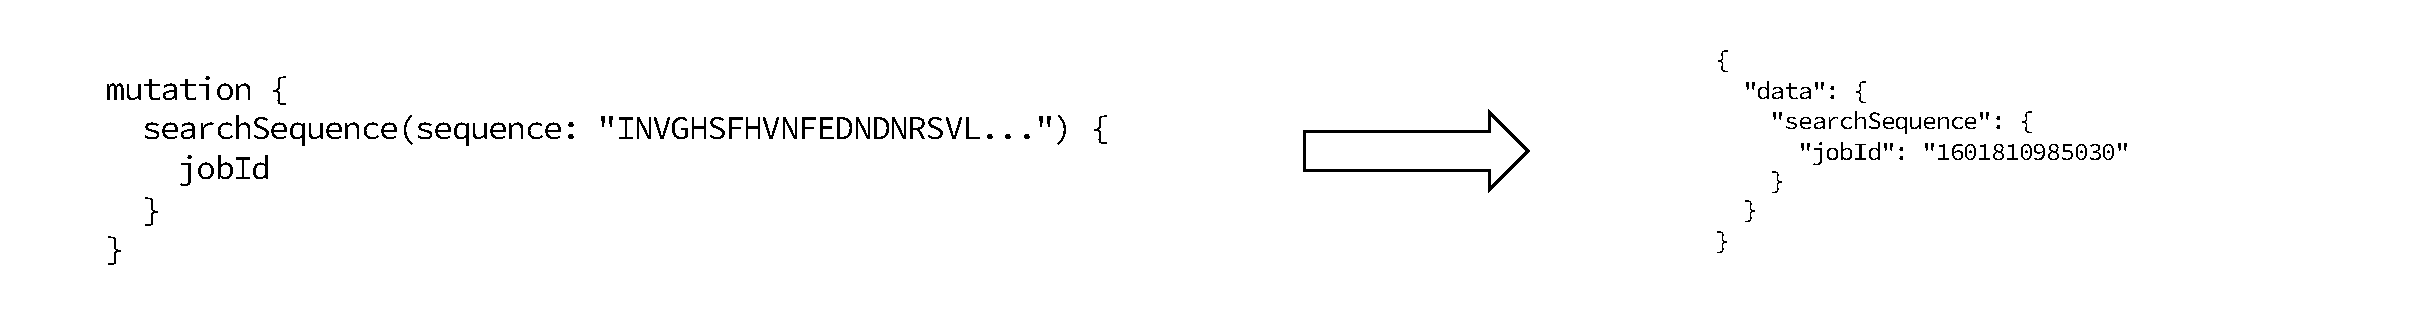
\includegraphics[width=1.0\textwidth]{Figures/zbp-mutation.eps}
\caption[ZincBindPredict mutation request.]{\label{fig:zbp-mutation} A mutation from the ZincBindPredict API. Mutations
begin with the mutation identifier to indicate that the top level \texttt{Mutation} object
is what the \texttt{searchSequence} mutation belongs to --- queries can begin with
\texttt{query} too but this is optional. Here the sequence is being given as an
argument, and the ID of the job is returned.}
\end{figure}

\begin{figure}
\centering
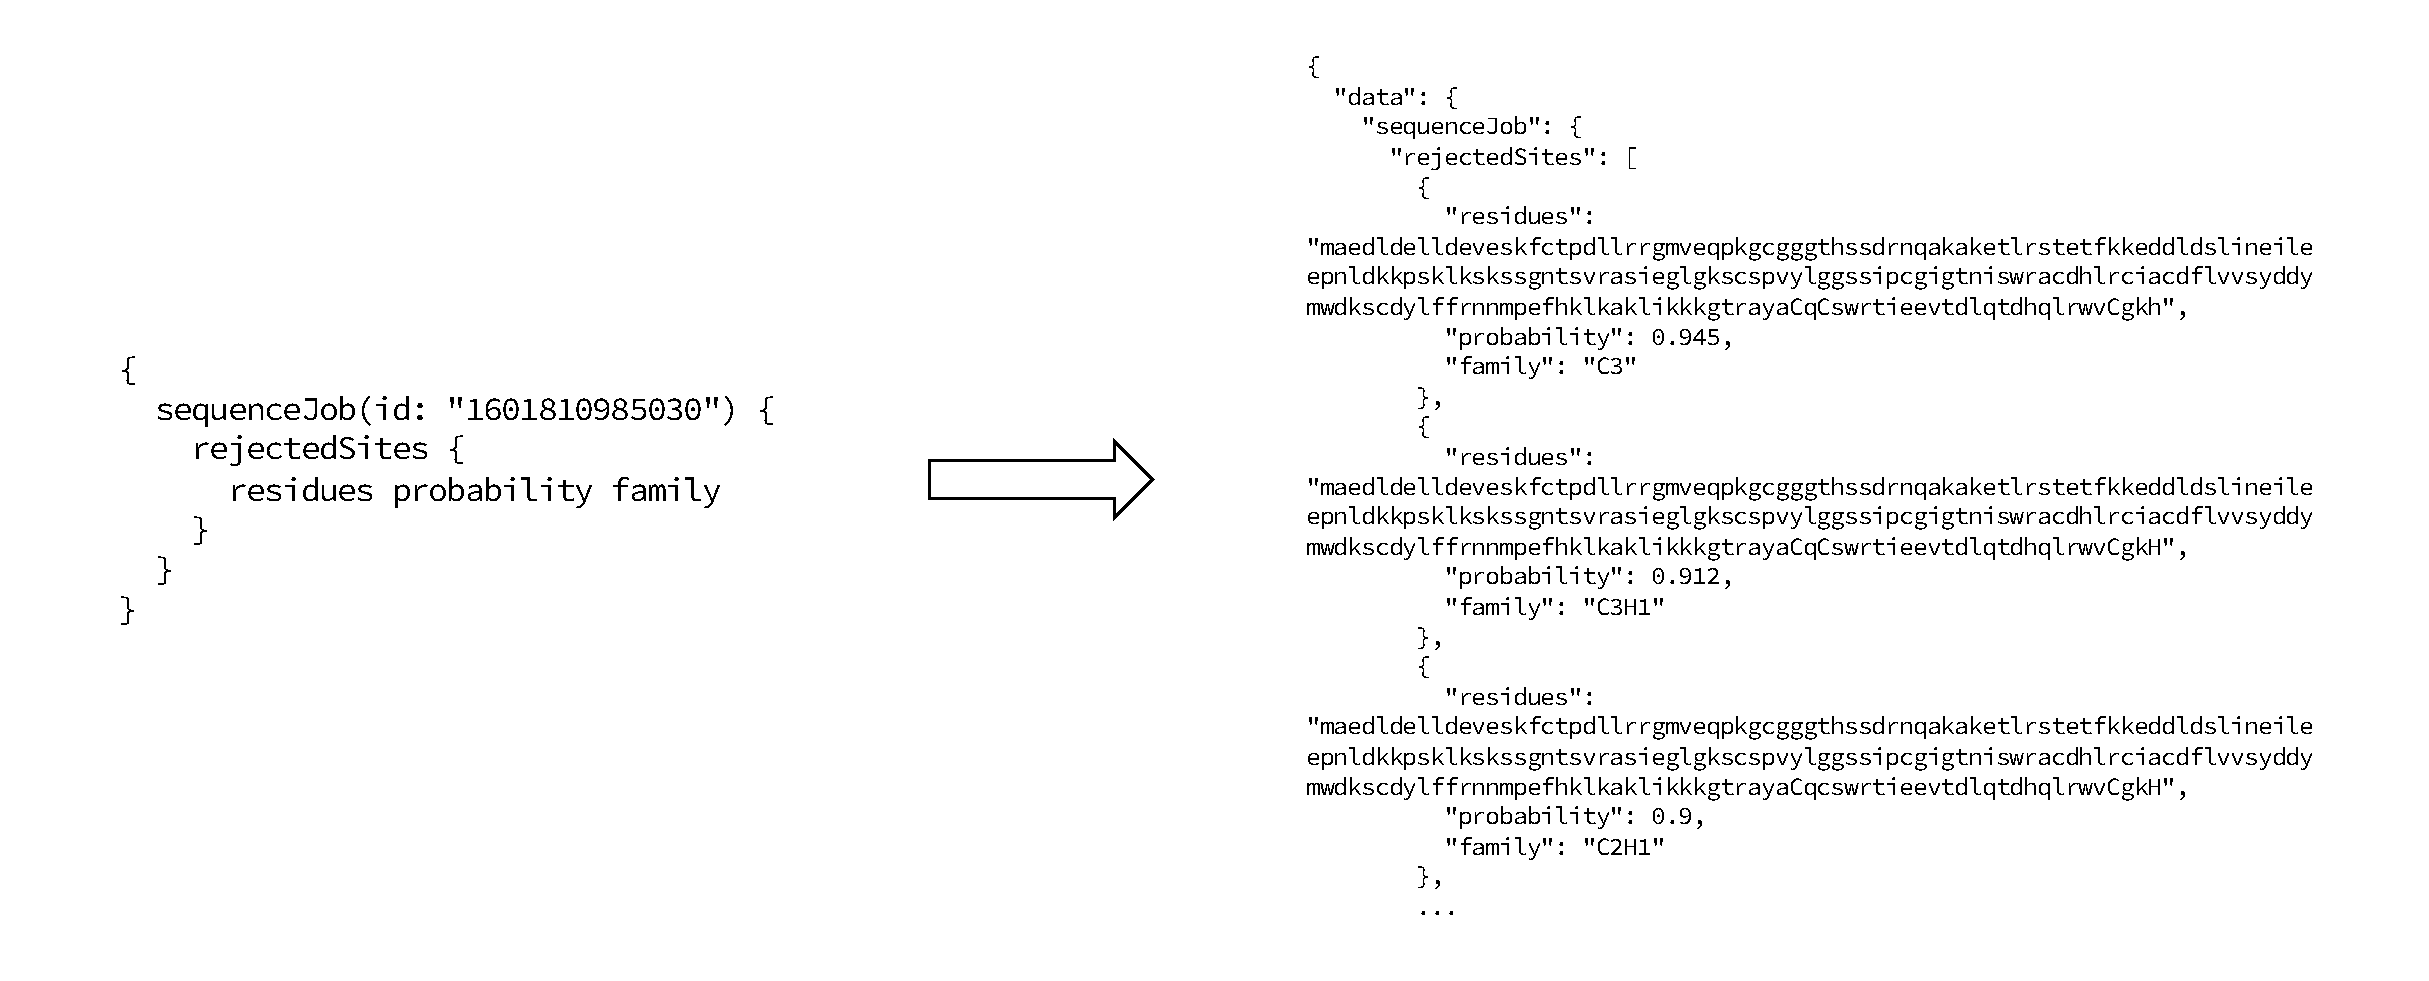
\includegraphics[width=1.0\textwidth]{Figures/zbp-query.eps}
\caption[ZincBindPredict query request.]{\label{fig:zbp-query} A query for the results of a ZincBindPredict job.
The ID of the job is supplied, and this particular query requests the status of
the job, as well the predicted sites. The rejected sites can also be requested,
but since they are quite numerous, typically the flexibility of GraphQL in allowing
you to choose to omit them is useful in conserving network resources.}
\end{figure}

\begin{figure}
\centering
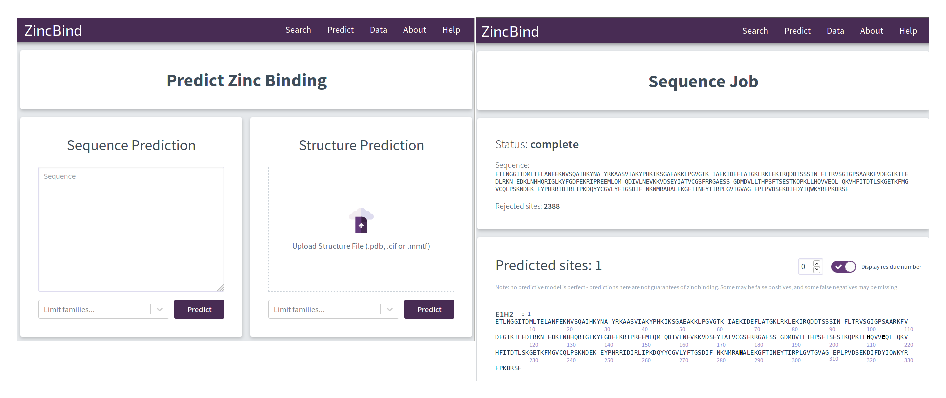
\includegraphics[width=1.0\textwidth]{Figures/prediction-interface.eps}
\caption[The prediction page on the ZincBind web interface.]{\label{fig:prediction-interface} The prediction page on the ZincBind web interface, and an example of a predicted zinc binding site in a protein sequence.}
\end{figure}

\section{Conclusion}

The models created here are highly effective, albeit at a very particular task. They are not predictors of zinc binding in general, and they will not generally detect zinc binding sites of obscure families and residue combinations. They were never intended to. A deliberate trade-off between model effectiveness and model generalisability has been made in order to demonstrate the principal that properties of binding sites within families \emph{are} more tightly distributed and hence create more accurate models. These models also detect something biologically real --- full binding sites --- rather than individual zinc binding residues which, as discussed, are an artificial concept.

However, this downside is not necessarily permanent. The models are limited to these ten models because these are the families for which there is sufficient (only just, in the case of some of the sequence models) data to train a classifier. However, the data in ZincBind is constantly growing thanks to the automated database update scripts in place. Over time, the eleventh-placed model will acquire enough data to warrant a model, and then the twelfth, and so on. The dataset-size threshold for training is not relative to the total size of the database, it is an absolute amount, and so over time more and more families will be able to have models trained for them, and the models will become more comprehensive of zinc binding generally. The benefits of this trade-off are permanent --- the deficiencies are temporary.
%%%% MACRO DEFINITION %%%%

\providecommand{\pvivax}{P.~vivax}
\providecommand{\pfalciparum}{P.~falciparum}
\providecommand{\cterm}{C-terminus}
\providecommand{\nterm}{N-terminus}

\providecommand{\e}[1]{\ensuremath{\times 10^{#1}}}
\newcolumntype{P}[1]{>{\centering\arraybackslash}p{#1}}
\newcolumntype{M}[1]{>{\centering\arraybackslash}m{#1}}

\providecommand{\refimage}[1]{\figurename~\ref{fig:#1}}

%TC:macro \note [ignore]



%%%%%%%%%%%%%%%%%%%%%%%%%%%%%%%%%%%%%%%%%%%%%%%%%%%%%%%%%%%%%%%%%%%%%%%%%%%%%%%%%%%%%%%%%%%%%%%%%%%%%%%%%%%%%%%%%%%%%
%%%%%%%%%%%%%%%%%%%%%%%%%%%%%%%%%%%%%%%%%%%%%%%%%%%%%%%%%%%%%%%%%%%%%%%%%%%%%%%%%%%%%%%%%%%%%%%%%%%%%%%%%%%%%%%%%%%%%
%													BEGIN
%%%%%%%%%%%%%%%%%%%%%%%%%%%%%%%%%%%%%%%%%%%%%%%%%%%%%%%%%%%%%%%%%%%%%%%%%%%%%%%%%%%%%%%%%%%%%%%%%%%%%%%%%%%%%%%%%%%%%
%%%%%%%%%%%%%%%%%%%%%%%%%%%%%%%%%%%%%%%%%%%%%%%%%%%%%%%%%%%%%%%%%%%%%%%%%%%%%%%%%%%%%%%%%%%%%%%%%%%%%%%%%%%%%%%%%%%%%

\chapter{Predicting Zinc Binding Sites between Chains} % Write in your own chapter title
\label{Chapter6}
\lhead{Chapter 6. \emph{Predicting Zinc Binding Sites between Chains}} % Write in your own chapter title to set the page header
%\include{Chapter_7}


%% ----------------------------------------------------------------
% Now begin the Appendices, including them as separate files

\addtocontents{toc}{\vspace{2em}} % Add a gap in the Contents, for aesthetics

\appendix % Cue to tell LaTeX that the following 'chapters' are Appendices

%%%% MACRO DEFINITION %%%%
% if any ...


%%%%%%%%%%%%%%%%%%%%%%%%%%%%%%%%%%%%%%%%%%%%%%%%%%%%%%%%%%%%%%%%%%%%%%%%%%%%%%%%%%%%%%%%%%%%%%%%%%%%%%%%%%%%%%%%%%%%%
%													BEGIN
%%%%%%%%%%%%%%%%%%%%%%%%%%%%%%%%%%%%%%%%%%%%%%%%%%%%%%%%%%%%%%%%%%%%%%%%%%%%%%%%%%%%%%%%%%%%%%%%%%%%%%%%%%%%%%%%%%%%%


\chapter{atomium} % Write in your own chapter title
\lhead{Appendix. \emph{A}} % Write in your own chapter title to set the page header

%TC:macro \note [ignore]

% write your code here
Much of this project relies very heavily on reading in structure data from files deposited to the Protein Data Bank.

Traditionally these files have been stored and distributed in the form of .pdb files. These are text files that consist of a list of records, with each record being limited to 80 characters. Information is stored in these records at fixed offsets from the start of the line. This file format has a number of limitations - most notably the fact that they cannot store more than 100,000 atoms because only five characters are allocated to atom IDs, and so they cannot go past 99,999.

Consequently, the Protein Data Bank also provides files in the newer .cif file format - and indeed, structures with more than 100,000 atoms are \emph{only} available in this file format.

There are a number of parsers available that can handle these file formats, and which were considered for use in this project - both in Python and otherwise. However, for reasons that will be outlined shortly, it was decided to create a novel Python parser. This parser is called atomium.

\section{Rationale}

The tool used to read structure files is of such critical importance to this project, that it was important to ensure that the correct tool with the correct \emph{capabilities} was used. Specifically, the tool would need the following properties:

\begin{itemize}
  \item The ability to read .pdb files.
  \item The ability to read .cif files.
\end{itemize}

Probably the major Python PDB parser at time of writing is BioPython. This is a multi-purpose bioinformatics library, with many modules for dealing with general biological data formats. One of these modules allows for parsing of PDB structure files.

\section{Data Structures}

The object returned by the various parsing functions is a \texttt{File} object. This essentially represents the actual file object itself rather than its structural contents, and has attributes for PDB code, resolution, keywords, etc.

A \texttt{File} object has one or more \texttt{Model} objects.

\section{Parsing}

\section{Saving}

One of the more unique features of atomium is that it allows changes to models to be made and then for those changes to be saved in \emph{any} of the three file types that atomium supports.

Unlike the process of parsing, in which the structures pass through a number of different representations reflecting the different layers of abstraction of that process, saving is much more starightforward. A function takes in an atomium \texttt{AtomStructure} (it doesn't need to be a model, chains etc. can be saved individually) and turns it into the relevant filestring.

Only structural information is saved - the various file annotations that are parsed from the original files are presumed to be properties solely of those original files, and not of any modified versions of them that might exist. So, atom records are saved, along with anything else needed to construct details of the actual structure model - but not titles, deposition dates, resolution etc.

\section{Usage}

%%%%%%%%%%%% END %%%%%%%%%%%%
	% Appendix Title
%%%% MACRO DEFINITION %%%%
% if any ...


%%%%%%%%%%%%%%%%%%%%%%%%%%%%%%%%%%%%%%%%%%%%%%%%%%%%%%%%%%%%%%%%%%%%%%%%%%%%%%%%%%%%%%%%%%%%%%%%%%%%%%%%%%%%%%%%%%%%%
%													BEGIN
%%%%%%%%%%%%%%%%%%%%%%%%%%%%%%%%%%%%%%%%%%%%%%%%%%%%%%%%%%%%%%%%%%%%%%%%%%%%%%%%%%%%%%%%%%%%%%%%%%%%%%%%%%%%%%%%%%%%%


\chapter{atomium Documentation} % Write in your own chapter title
\lhead{Appendix. \emph{B}} % Write in your own chapter title to set the page header

%TC:macro \note [ignore]

% write your code here
atomium is a Python library for opening and saving .pdb, .cif and .mmtf files,
and presenting and manipulating the information contained within. The rationale behind its development and details of its core concepts were outlined in Chapter 3 --- this Appendix gives examples of its use in practice. The full documentation is at \url{atomium.bio}.

\section{Loading Data}

While you can use atomium to create models from scratch to build an entirely \emph{de novo} structure, in practice you would generally use it to load molecular data from an existing file...

\begin{footnotesize}
\begin{verbatim}
>>> import atomium
>>> pdb1 = atomium.open(`../1LOL.pdb')
>>> mmtf1 = atomium.open(`/structures/glucose.mmtf')
>>> cif1 = atomium.open(`/structures/1XDA.cif')
>>> pdb3 = atomium.open(`./5CPA.pdb.gz')
>>> pdb2 = atomium.fetch(`5XME.pdb')
>>> cif2 = atomium.fetch(`5XME')
\end{verbatim}
\end{footnotesize}

In that latter case, you don't need the file to be saved locally --- it will just go and grab the PDB with that code from the RCSB.

atomium will use the file extension you provide to decide how to parse it. If there isn`t one, or it doesn't recognise the extension, it will peek at the file contents and try and guess whether it should be interpreted as .pdb, .cif or .mmtf.

\section{Using Data}

Once you've got your File object, what can you do with it?

\subsection{Annotation}

There is meta information contained within the File object:

\begin{footnotesize}
\begin{verbatim}
>>> pdb1.title
`CRYSTAL STRUCTURE OF OROTIDINE MONOPHOSPHATE DECARBOXYLASE COMPLEX WITH XMP'
>>> pdb1.deposition_date
datetime.date(2002, 5, 6)
>>> pdb1.keywords
[`TIM BARREL`, `LYASE']
>>> pdb1.classification
`LYASE'
>>> pdb1.source_organism
`METHANOTHERMOBACTER THERMAUTOTROPHICUS STR. DELTA H'
>>> pdb1.resolution
1.9
>>> pdb1.rvalue
0.193
>>> pdb1.rfree
0.229
\end{verbatim}
\end{footnotesize}

\subsection{Models and Assembly}

All .pdb files contain one or more models --- little universes containing a
molecular scene.

\begin{footnotesize}
\begin{verbatim}
>>> pdb1.model
<Model (2 chains, 4 ligands)>
>>> pdb1.models
(<Model (2 chains, 4 ligands)>,)
\end{verbatim}
\end{footnotesize}

Most just contain one --- it's generally those that come from NMR experiments which contain multiple models. You can easily iterate through these to get their individual metrics:

\begin{footnotesize}
\begin{verbatim}
>>> for model in pdb2.models:
    print(model.center_of_mass)
\end{verbatim}
\end{footnotesize}

This model contains the `asymmetric unit' --- this is one or more protein
(usually) chains arranged in space, which may not be how the molecule arranges
itself in real life. It might just be how they arranged themselves in the
experiment. To create the `real thing' from the asymmetric unit, you use
\emph{biological assemblies}.

Most .pdb files contain one or more biological assemblies --- instructions for how
to create a more realistic structure from the chains present, which in atomium
are accessed using \texttt{File.assemblies}.

In practice, what you need to know is that you can create a new model (not the
one already there containing the asymmetric unit) as follows...

\begin{footnotesize}
\begin{verbatim}
>>> pdb3 = atomium.fetch(`1XDA')
>>> pdb3.model
<Model (8 chains, 16 ligands)>
>>> pdb3.generate_assembly(1)
<Model (2 chains, 4 ligands)>
>>> pdb3.generate_assembly(10)
<Model (6 chains, 12 ligands)>
>>> [pdb.generate_assembly(n + 1) for n in range(len(pdb.assemblies))]
[<Model (2 chains, 4 ligands)>, <Model (2 chains, 4 ligands)>, <Model (2 cha
ins, 4 ligands)>, <Model (2 chains, 4 ligands)>, <Model (12 chains, 24 ligan
ds)>, <Model (12 chains, 24 ligands)>, <Model (6 chains, 12 ligands)>, <Mode
l (6 chains, 12 ligands)>, <Model (6 chains, 12 ligands)>, <Model (6 chains,
 12 ligands)>, <Model (4 chains, 8 ligands)>, <Model (4 chains, 8 ligands)>]
\end{verbatim}
\end{footnotesize}

Here you load a .pdb with multiple possible assemblies, have a quick look at
the asymmetric unit with 1,842 atoms, and then generate first , and then all,
of its possible biological assemblies by passing in their IDs.

\subsection{Model Contents}

The basic structures within a model are chains, residues, ligands, and atoms.

\begin{footnotesize}
\begin{verbatim}
>>> pdb1.model.chains()
{<Chain A (204 residues)>, <Chain B (214 residues)>}
>>> pdb1.model.chain(`B')
<Chain B (214 residues)>
>>> pdb1.model.residues(name=`TYR')
{<Residue TYR (A.37)>, <Residue TYR (B.1037)>, <Residue TYR (A.45)>, <Residu
e TYR (A.154)>, <Residue TYR (B.1206)>, <Residue TYR (B.1154)>, <Residue TYR
 (B.1045)>, <Residue TYR (A.206)>}
>>> pdb1.model.residues(name__regex=`TYR|PRO')
{<Residue PRO (A.101)>, <Residue PRO (A.46)>, <Residue PRO (A.161)>, <Residu
e TYR (A.45)>, <Residue PRO (B.1046)>, <Residue TYR (A.154)>, <Residue TYR (
B.1206)>, <Residue TYR (B.1045)>, <Residue PRO (B.1189)>, <Residue TYR (A.37
)>, <Residue PRO (B.1129)>, <Residue PRO (B.1077)>, <Residue PRO (A.211)>, <
Residue PRO (B.1180)>, <Residue PRO (B.1157)>, <Residue PRO (B.1211)>, <Resi
due PRO (B.1228)>, <Residue PRO (B.1101)>, <Residue TYR (B.1154)>, <Residue
PRO (A.157)>, <Residue PRO (A.77)>, <Residue PRO (A.180)>, <Residue TYR (B.1
037)>, <Residue PRO (A.129)>, <Residue PRO (B.1161)>, <Residue TYR (A.206)>}
>>> pdb1.model.chain(`B`).residue(`B.1206')
<Residue TYR (B.1206)>
>>> pdb1.model.chain(`B`).residue(`B.1206').helix
True
>>> pdb1.model.ligands()
{<Ligand BU2 (A.5001)>, <Ligand XMP (A.2001)>, <Ligand BU2 (B.5002)>, <Ligan
d XMP (B.2002)>}
>>> pdb1.model.ligand(name=`BU2').atoms()
{<Atom 3196 (O3)>, <Atom 3192 (C1)>, <Atom 3193 (O1)>, <Atom 3197 (C4)>, <At
om 3194 (C2)>, <Atom 3195 (C3)>}
>>> pdb1.model.ligand(name=`BU2').atoms(mass__gt=12)
{<Atom 3196 (O3)>, <Atom 3192 (C1)>, <Atom 3193 (O1)>, <Atom 3197 (C4)>, <At
om 3194 (C2)>, <Atom 3195 (C3)>}
>>> pdb1.model.ligand(name=`BU2').atoms(mass__gt=14)
{<Atom 3196 (O3)>, <Atom 3193 (O1)>}
\end{verbatim}
\end{footnotesize}


The examples above demonstrate atomium's selection language. In the case of the
molecules --- Model, Chain, \texttt{Residue} and
\texttt{Ligand} --- you can pass in an \texttt{id} or \texttt{name}, or search by regex
pattern with \texttt{id\_\_regex} or \texttt{name\_\_regex}.

These structures have an even more powerful syntax too --- you can pass in \emph{any}
property such as \texttt{charge=1}, any comparitor of a property such as
\texttt{mass\_\_lt=100}, or any regex of a property such as \texttt{name\_\_regex=`[\^C]'}.

For pairwise comparisons, structures also have the
\texttt{.AtomStructure.pairwise\_atoms} generator which will yield all
unique atom pairs in the structure. These can obviously get very big indeed --- a
5000 atom PDB file would have about 12 million unique pairs.

Structures can be moved around and otherwise compared with each other...

\begin{footnotesize}
\begin{verbatim}
pdb1.model.ligand(id=`B:2002').mass
351.1022
>>> pdb1.model.ligand(id=`B.2002').formula
Counter({`C': 10, `O': 9, `N': 4, `P': 1})
>>> pdb1.model.ligand(id=`B:2002').nearby_atoms(2.8)
{<Atom 3416 (O)>, <Atom 3375 (O)>, <Atom 1635 (OD1)>}
>>> pdb1.model.ligand(id=`B.2002').nearby_atoms(2.8, name=`OD1')
{<Atom 1635 (OD1)>}
>>> pdb1.model.ligand(id=`B.2002').nearby_residues(2.8)
{<Residue ASP (B.1020)>}
>>> pdb1.model.ligand(id=`B.2002').nearby_structures(2.8, waters=True)
{<Residue ASP (B.1020)>, <Water HOH (B.3155)>, <Water HOH (B.3059)>}
>>> import math
>>> pdb1.model.ligand(id=`B.2002').rotate(math.pi / 2, `x')
>>> pdb1.model.ligand(id=`B.2002').translate(10, 10, 15)
>>> pdb1.model.ligand(id=`B.2002').center_of_mass
(-9.886734282781484, -42.558415679537184, 77.33400578435568)
>>> pdb1.model.ligand(id=`B.2002').radius_of_gyration
3.6633506511540825
>>> pdb1.model.ligand(id=`B.2002').rmsd_with(pdb1.model.ligand(id=`A.2001'))
0.133255572356
\end{verbatim}
\end{footnotesize}

Here we look at one of the ligands, identify its mass and molecular formula,
look at what atoms are within 2.8 \AA of it, and what residues are within
that same distance, rotate it and translate it through space, see where its new
center of mass is, and then finally get its RMSD with the other similar ligand
in the model.

Any operation which involves identifying nearby structures or atoms can be sped
up --- dramatically in the case of very large structures --- by calling
\texttt{.Model.optimise\_distances} on the \texttt{Model} first. This
prevents atomium from having to compare every atom with every other atom every
time a proximity check is made.

The \texttt{Atom} objects themselves have their own useful properties.

\begin{footnotesize}
\begin{verbatim}
>>> pdb1.model.atom(97)
<Atom 97 (CA)>
>>> pdb1.model.atom(97).mass
12.0107
>>> pdb1.model.atom(97).anisotropy
[0, 0, 0, 0, 0, 0]
>>> pdb1.model.atom(97).bvalue
24.87
>>> pdb1.model.atom(97).location
(-12.739, 31.201, 43.016)
>>> pdb1.model.atom(97).distance_to(pdb1.model.atom(1))
26.18289982030257
>>> pdb1.model.atom(97).nearby_atoms(2)
{<Atom 96 (N)>, <Atom 98 (C)>, <Atom 100 (CB)>}
>>> pdb1.model.atom(97).is_metal
False
>>> pdb1.model.atom(97).structure
<Residue ASN (A.23)>
>>> pdb1.model.atom(97).chain
<Chain A (204 residues)>
\end{verbatim}
\end{footnotesize}

Chains are a little different from other structures in that they are iterable,
indexable, and return their residues as a tuple, not a set...

\begin{footnotesize}
\begin{verbatim}
>>> pdb1.model.atom(97).chain
<Chain A (204 residues)>
>>> pdb1.model.chain(`A')
<Chain A (204 residues)>
>>> len(pdb1.model.chain(`A'))
204
>>> pdb1.model.chain(`A')[10]
<Residue LEU (A.21)>
>>> pdb1.model.chain(`A').residues()[:5]
(<Residue VAL (A.11)>, <Residue MET (A.12)>, <Residue ASN (A.13)>, <Residue
ARG (A.14)>, <Residue LEU (A.15)>)
>>> pdb1.model.chain(`A').sequence
`LRSRRVDVMDVMNRLILAMDLMNRDDALRVTGEVREYIDTVKIGYPLVLSEGMDIIAEFRKRFGCRIIADFKVAD
IPETNEKICRATFKAGADAIIVHGFPGADSVRACLNVAEEMGREVFLLTEMSHPGAEMFIQGAADEIARMGVDLGV
KNYVGPSTRPERLSRLREIIGQDSFLISPGVGAQGGDPGETLRFADAIIVGRSIYLADNPAAAAAGIIESIKDLLI'
\end{verbatim}
\end{footnotesize}

The sequence is
the `real' sequence that exists in nature. Some of them will be
missing from the model for practical reasons.

Residues can generate name information based on their three letter code, and are
aware of their immediate neighbors.

\begin{footnotesize}
\begin{verbatim}
>>> pdb1.model.residue(`A.100')
<Residue PHE (A.100)>
>>> pdb1.model.residue(`A.100').name
`PHE'
>>> pdb1.model.residue(`A.100').code
`F'
>>> pdb1.model.residue(`A.100').full_name
`phenylalanine'
>>> pdb1.model.residue(`A.100').next
<Residue PRO (A.101)>
>>> pdb1.model.residue(`A.100').previous
<Residue GLY (A.99)>
\end{verbatim}
\end{footnotesize}

\section{Saving Data}

A model can be saved to file using:

\begin{footnotesize}
\begin{verbatim}
>>> model.save(`new.cif')
>>> model.save(`new.pdb')
\end{verbatim}
\end{footnotesize}

Any structure can be saved in this way, so you can save chains or molecules to
their own seperate files if you so wish.

\begin{footnotesize}
\begin{verbatim}
>>> model.chain(`A').save(`chainA.pdb')
>>> model.chain(`B').save(`chainB.cif')
>>> model.ligand(name=`XMP').save(`ligand.mmtf')
\end{verbatim}
\end{footnotesize}

Note that if the model you are saving is one from a biological assembly, it will
likely have many duplicated IDs, so saving to file may create unexpected
results.


%%%%%%%%%%%% END %%%%%%%%%%%%



\addtocontents{toc}{\vspace{2em}}  % Add a gap in the Contents, for aesthetics
\backmatter

%% ----------------------------------------------------------------
\label{Bibliography}
\lhead{\emph{Bibliography}}  % Change the left side page header to "Bibliography"
%\bibliographystyle{unsrtnat}  % Use the "unsrtnat" BibTeX style for formatting the Bibliography
\bibliographystyle{ieeetr}  % Use the "unsrtnat" BibTeX style for formatting the Bibliography
\bibliography{Bibliography}  % The references (bibliography) information are stored in the file named "Bibliography.bib"

\end{document}  % The End
%% ----------------------------------------------------------------
